\chapter{Grammaticality intuitions}

The use of \isi{grammaticality} intuitions as empirical data in linguistic theory is controversial, and there is an ongoing debate regarding their utility (\citealt{CulicoverJackendoff2010,FFerreira2005,GibsonFedorenko2010,GibsonFedorenko2013,SprouseAlmeida2013}). Conventionally, \isi{grammaticality} is distinguished from \isi{acceptability} (\citealt{Schütze2016,Sprouse2007}). \isi{Grammaticality} is said to relate to “competence”, i.e. knowledge of an underlying grammar, the isolated “narrow” faculty of language. Acceptability relates to intuitions regarding whether sentences are “acceptable” (i.e. something a \isi{speaker} could say and/or understand), and these intuitions are presumed to derive from \isi{grammaticality} intuitions plus other “performance” factors: memory limitations, semantic plausibility, \isi{interpreter} age, emotional state, etc. 

  There are serious problems with the distinction between \isi{grammaticality} and \isi{acceptability}. For the distinction to make any sense, one has to presuppose some concept of a grammar and an isolated syntax module. There is also the issue of whether it is possible empirically to distinguish \isi{grammaticality} intuitions from \isi{acceptability} intuitions. Because of these problems we deliberately conflate \isi{grammaticality} and \isi{acceptability} in the o/el approach. In the o/el model, production and interpretation are associated with trajectories in a \isi{state space}, and meanings are experiences of those trajectories. \isi{Grammaticality} intuitions thus cannot be intuitions \textit{about objects}, in this view. Instead, \isi{grammaticality} intuitions must be experiences of trajectories. The question then becomes: what determines the quality of those experiences? 

  We propose below that \isi{grammaticality}/\isi{acceptability} intuitions arise from the experience of system \isi{coherence}. As shown earlier, for a coherent system, the width of the peak in its power spectrum is relatively narrow and the peak remains at a constant frequency. These properties are required for stability. \isi{Grammaticality}/\isi{acceptability} intuitions can thus be understood in relation to the \isi{coherence} of all systems for all excited ϕ-con\-fi\-gu\-ra\-tions in a trajectory, which we call \textit{grammatical coherence}. In this chapter, we develop a heuristic test of \isi{grammatical coherence} which involves assessing whether a trajectory can be reiterated, apply the concept of \isi{coherence} to intuitions regarding \isi{constituency}, and examine some electrophysiological manifestations of \isi{coherence}. 

\section{Problems with grammaticality}

The conventional concepts of \isi{grammaticality} and \isi{acceptability} are easy targets for critique. We elaborate several such critiques here: (i) \isi{grammaticality} and grammar can only be defined circularly; (ii) intuitions are inherently dynamic but often treated as static; (iii) the mechanisms behind \isi{grammaticality} intuitions conflate producer and \isi{interpreter} states; (iv) intuitions have often been associated with only sentences or phrases, but they are unavoidably associated with context as well.

\subsection{Grammar-grammaticality circularity}

The concepts of \textit{a grammar} and \textit{a grammatical sentence} form a tautological relation with \isi{grammaticality} intuitions. One view of a grammar evokes the \textit{grammar-as-theory} motif:

\begin{quote}
The grammar of a language can be viewed as a theory of the structure of this language. Any scientific theory is based on a certain finite set of observations and, by establishing general laws stated in terms of certain hypothetical constructs, it attempts to account for observations, to show how they are interrelated, and to predict an indefinite number of new phenomena. \citep[113]{Chomsky1956}
\end{quote}

  The above view fails to recognize that there is no theory-free observation nor theory-neutral conception of “the structure”. The observations themselves are always theoretical constructs. Conceptual metaphors and image schemas unavoidably predetermine our understanding of the observations. One might take a \textit{so what?} attitude to this critique -- perhaps the point that observations are never theory-free is obvious and inescapable and we can shrug it off and get on with our lives. Even so, the above passage begs the question of \textit{what} the observations \textit{are}. We should always attend to the process of constructing our understanding of the observations, because the theory and observations are one and the same.

  Whereas \textit{grammar-as-theory} views the grammar itself as the theory, \textit{grammar-as-device} views a grammar as an object that is studied by theory. This serves to reify the notion of a grammar; grammars become entities which we study:

\begin{quote}
Syntactic investigation of a given language has as its goal the construction of a grammar that can be viewed as a device of some sort for producing the sentences of the language under analysis. …The ultimate outcome of these investigations should be a theory of linguistic structure in which the descriptive devices utilized in particular grammars are presented and studied abstractly, with no specific reference to particular languages. \citep[11]{Chomsky1957}
\end{quote}

A fairly reasonable expectation, for a scientific discipline, is that a grammar must explain behavior:

\begin{quote}
…a grammar must reflect and explain the ability of a \isi{speaker} to produce and understand new sentences which may be much longer than any he has previously heard. \citep[124]{Chomsky1956}
\end{quote}

  But the above uses of \textit{grammar} presuppose that we can know what “the sentences of the language” and “new sentences” \textit{are}. How do we know which sentences are grammatical, and which ones are not? Sometimes the distinction is assumed to be evident:

\begin{quote}
…a device of some sort (called a grammar) for generating all and-only-the sentences of a language, which we have assumed were somehow given in advance. \citep[85]{Chomsky1957}

Suppose that for many languages there are certain clear cases of grammatical sentences and certain clear cases of \isi{ungrammatical} sequences. \citep[113]{Chomsky1956}

…we may assume for this discussion that certain sequences of phonemes are definitely sentences, and that certain other sequences are definitely non-sentences. \citep[14]{Chomsky1957}
\end{quote}

Clearly, one would like to provide more empirically grounded definitions, or a method for determining which sentences are and are not in the set of grammatical ones:

\begin{quote}
One way to test the adequacy of a grammar proposed for L [\textit{a set of sentences}] is to determine whether or not the sequences that it generates are actually grammatical, i.e., acceptable to a native \isi{speaker}, etc. We can take certain steps towards providing a behavioral criterion for grammaticalness so that this test of adequacy can be carried out. For the purposes of this discussion, however, suppose that we assume intuitive knowledge of the grammatical sentences of English and ask what sort of grammar will be able to do the job of producing these in some effective and illuminating way. We thus face a familiar task of explication of some intuitive concept -- in this case, the concept “grammatical in English,” and more generally, the concept “grammatical”. \citep[13]{Chomsky1957}.
\end{quote}

  A skeptic might be wary of the “intuitive concept” but nonetheless excited to explore the “behavioral criterion for grammaticalness”. One such criterion involves how sentences are read. Regarding sentences with structures analogous to \REF{ex:6:1} and \REF{ex:6:2} below, \citet{Chomsky1956} identified \isi{intonation} as one such behavioral criterion:

\begin{quote} 
  
\ea\label{ex:6:1}
Al ate a sandwich.
\z


\ea\label{ex:6:2}
Sandwich a ate Al%\todo{we can probably keep NC's numbering here since it is the first example in this chapter}
\z

\REF{ex:6:1} will be read by an English \isi{speaker} with the normal \isi{intonation} of a sentence of the corpus, while \REF{ex:6:2} will be read with a falling \isi{intonation} on each word, as will any sequence of unrelated words \citep[114]{Chomsky1956}.

\end{quote}


  But the occurrence of \isi{list intonation} cannot be either a necessary or sufficient criterion for \isi{grammaticality}: sentence \REF{ex:6:1} \text{can} be uttered with \isi{list intonation}, and \REF{ex:6:2} \textit{can} be uttered with phrasal \isi{intonation}. Indeed, plenty of “grammatical” sentences like \REF{ex:6:3} would probably exhibit a strong tendency to be read with \isi{list intonation}: 

\ea\label{ex:6:3}
\textit{A frog a cat a dog chased scared jumped far.}
\z

Some additional \isi{prosodic} criteria are mentioned in a footnote of \citet{Chomsky1957}, in reference to \REF{ex:6:4}:

\ea\label{ex:6:4}
\textit{John enjoyed the book and liked the play}
\z

\begin{quote}
Such sentences with conjunction crossing constituent boundaries are also, in general, marked by special phonemic features such as extra long pauses (in our example, between ``liked" and ``the"), contrastive stress and \isi{intonation}, failure to reduce vowels and drop final consonants in rapid speech, etc. Such features normally hark the reading of non-grammatical strings. \citep[35-36]{Chomsky1957}
\end{quote}

Prosodic and other \isi{phonological} criteria are problematic justifications for \linebreak\isi{grammaticality}, at least in the prevailing theoretical frame, because the \isi{narrow language faculty} is supposed to be isolated from the \isi{sensorimotor} interfaces. This is likely why such criteria seem to have been abandoned in subsequent work. Or perhaps gestural-motoric aspects of production were subsequently understood to be too complex and variable to serve as useful criteria. An alternative basis for empirical determination of \isi{grammaticality} involves associating “grammatical sentences” with “observed sentences”:

\begin{quote}	
  Notice that to meet the aims of grammar, given a linguistic theory, it is sufficient to have a partial knowledge of the sentences (i.e., a corpus) of the language, since a linguistic theory will state the relation between the set of observed sentences and the set of grammatical sentences; i.e., it will define “grammatical sentence” in terms of “observed sentence”, certain properties of the observed sentences, and certain properties of grammars. \citep[14]{Chomsky1957}.
\end{quote}

  This is different from the \isi{intonational}/\isi{phonological} criteria, but quite problematic for other reasons. First, what is meant by \textit{observed}? Is an observed sentence a sentence that is produced by a native \isi{speaker}? Surely observation is not sufficient for \isi{grammaticality}, since native speakers do produce “\isi{ungrammatical}” sentences through \isi{disfluency} mechanisms. And, observation cannot be a necessary condition, since plenty of grammatical utterances are never observed. In that case, perhaps intuition can guide us in deciding which observations and non-observations to include:
  
\begin{quote}	
It is undeniable that intuition about linguistic form is very useful to the investigator of linguistic form (i.e., grammar). It is also quite clear that the major goal of grammatical theory is to replace this obscure reliance on intuition by some rigorous and objective approach. \citep[93-94]{Chomsky1957}
\end{quote}

  Many references to \isi{grammaticality} show awareness of the tension between the theoretically dichotomous character of \isi{grammaticality} and the complex, non-dichotomous nature of \isi{grammaticality} intuitions. Notice that in a previous excerpt reference was made to “certain clear cases” of \isi{ungrammatical} sequences \citep[113]{Chomsky1956}. The need to qualify some cases as \textit{clear} cases, implies that some cases are \textit{unclear}. This contradicts the idea that a language can be understood as a set of grammatical sentences. Indeed, Chomsky explicitly refers to degrees of grammaticalness: 

\begin{quote}	
…the resulting sentences are semi-grammatical; the more completely we violate constituent structure by conjunction, the less grammatical is the resulting sentence. This description requires that we generalize the grammatical/\isi{ungrammatical} dichotomy, developing a notion of degree of grammaticalness \citep[36]{Chomsky1957}.
\end{quote}

\begin{quote}	
…we may assume for this discussion that certain sequences of phonemes are definitely sentences, and that certain other sequences are definitely non-sentences. In many intermediate cases we shall be prepared to let the grammar itself decide, when the grammar is set up in the simplest way so that it includes the clear sentences and excludes the clear non-sentences \citep[14]{Chomsky1957}.
\end{quote}

  What are these “intermediate cases” that straddle the dichotomy between\linebreak grammatical and nongrammatical sentences? Ultimately, the problem is that the theoretical constructs -- i.e. language as a set (container) of sentences (objects) -- requires precise definition of which objects are inside and outside (members and non-members) of the set, but our intuitions about \isi{grammaticality} cannot be categorized so simply.

  From the above we see that \isi{grammaticality} is defined relative to a presupposed grammar, and a grammar is defined from observations of \isi{grammaticality} or tenuous correlates thereof. There is a disconnect between the discrete intuitions predicted by a grammar and the messiness of actual intuitions. The conventional solution to this problem evolved from “degrees of grammaticalness” into a distinction between \isi{grammaticality} and \isi{acceptability}, but the circularity problem has never been resolved. 

\subsection{The non-stationarity of intuitions}

Another major problem with \isi{grammaticality} is that intuitions are commonly treated as static rather than dynamic. Simply put, our intuitions can change over time and may never be stable. To illustrate, read the sentence below \textit{at a normal pace}, \textit{just one time through}:

\ea
    {Either either Dee or Cam knows or Bo knows that Al drinks coffee.}
\z    

On first read-through, assuming you did not backtrack, you probably did not reach any clear understanding of the meaning of the sentence. Backtracking is quite natural, and you might have backtracked subconsciously without realizing it. Now consider the sentence again, with punctuation to help:

\ea
Either, either Dee or Cam knows, or Bo knows, that Al drinks coffee.
\z

  Read the sentence bit by bit, over and over again, until you understand it. Diagram it out with a Venn diagram or decision tree if you need to. Eventually, it should make some sense. You would never say this sentence (probably), but you can achieve an understanding of it with some effort. Your intuitions about the sentence have changed. This example shows that intuitions are not static, but rather, dynamic, i.e. intuitions change over time.

  Is the time evolution of intuitions predictable? Let's assume that changes such as above are due to the “other factors” (e.g. memory limitations), which are conventionally associated with \isi{acceptability}. Your early intuitions were muddled by these other factors, and with some effort, the intuition (experience) became stable. Perhaps this is always the pattern: with enough effort, a grammatical sentence which is initially unacceptable becomes acceptable through practice, which can be viewed as a satiation effect \citep{Snyder2000}. Let's consider another example:

\ea
Which coffee\textsubscript{i} does its\textsubscript{i} brewer drink t\textsubscript{i}?
\z

  The target interpretation here is one in which the \isi{pronoun} \textit{its} refers to the coffee that the brewer of that same coffee drinks. If you are unfamiliar with this sort of pattern (known as \isi{weak crossover}) and ignored the coindexation, your initial interpretation most likely assumed some antecedent other than \textit{coffee} for \textit{its}. If so, try to obtain the target \isi{weak crossover} interpretation. To do this, read the sentence slowly, and when you get to the possessive \isi{pronoun} \textit{its}, remember that \textit{its} refers to the coffee in question. Imagining a context may help as well:

\ea
\begin{exe}
\exi{P1:}  {Bo brews D-flavored coffee but does not drink it. Al brews C-flavored coffee and drinks it too.} 
\exi{P2:}  {Wait -- which coffee does its brewer drink?}
\end{exe}
\z

  Hopefully you can achieve the target \isi{weak crossover} meaning. If so, your interpretation has evolved over time. We cannot say that the original difficulty was due to “memory limitations,” since the sentence is not particularly long and the non-crossover version is quite easy to process. 

  After learning the \isi{weak crossover} interpretation, does the \isi{meaning experience} reach a steady state? Read the sentence 20 times, and after each reading take a moment to reflect on what the sentence means. What happens to your intuitions? Most likely they are not the same after the twentieth reading as after the first. Set an alarm for 24 hours from now, or ask someone to remind you tomorrow, and read the sentence (you will probably remember it, so just rehearse it). When you do this, will your intuitions be the same as they are now? Probably not. Let's consider another weak-crossover sentence: 

\ea
Which brewer\textsubscript{i} does his\textsubscript{i} coffee please t\textsubscript{i}?
\z

  Your practice with the previous example may help you achieve the \isi{crossover interpretation} more quickly with this new example, but perhaps not immediately. You may still need to put in some effort. What would happen if you practiced a new \isi{weak crossover} sentence every day, over the next year? Would the dynamics of your intuitions change? Certainly. Perhaps you could eventually come to judge strong crossover sentences as acceptable (e.g. \textit{Who\textsubscript{i} did he\textsubscript{i} brew coffee for\textsubscript{i}}?). 

  The multi-timescale nature of intuition dynamics, and interactions between intuitions of different utterances, show that intuition changes are not simple approximations to a steady state. The evolution of intuitions is not merely the result of overcoming the influence of the “other factors”. Indeed, there is no reason to assume that intuitions are ever stable. The observation that linguists exhibit different intuitions than non-linguists \citep{Spencer1973} further supports the conclusion that intuitions are inherently unstable in the presence of certain \isi{surroundings} forces, such as doctoral training in linguistics. It raises the question of whether even more extreme training (e.g. a \isi{crossover interpretation} boot camp) can radically alter intuitions. The conventional perspective in which \isi{grammaticality} intuitions are presumed not to change (because grammars should be static), while \isi{acceptability} intuitions can change, is ultimately not satisfactory. The problem with partitioning intuitions in this way is that, if the grammar is independent of other systems, then all of the rich dynamics of intuition that do occur, i.e. changes driven by practice, learning, time, context, etc., cannot inform our understanding of “the grammar”.

\subsection{Conflating production and interpretation}

Another problem with notions of \isi{grammaticality} and \isi{acceptability} is conflation of production and interpretation. Production involves speaking, signing, and\linebreak writing; interpretation involves listening, sign-viewing, and reading. We expect these various activities to differ due to differential involvement of sensory and motor systems, but we also expect production and interpretation to interact. In many circumstances, speakers monitor their own speech, and conversely hearers rehearse/simulate the utterances they hear. The problem with the conventional approach to understanding intuitions is that it does not provide useful tools for disentangling production and interpretation.

  Let's reflect some more on an example we considered previously. How do production and interpretation contribute to changes in our intuitions regarding the following sentence? 

\ea
Either either Dee knows or Cam knows or Bo knows that Al drinks coffee.
\z

  On first reading, you probably did not understand the sentence. The mechanisms which are normally involved in interpretation created a state which you experienced as somehow abnormal. So, you engaged production mechanisms: you produced the utterance slowly, either in a \isi{subvocal rehearsal} mode (i.e. with execution gated) or out loud. This may have helped you keep track of various relational meanings evoked in the utterance. On your next attempt at interpretation, you came closer to understanding the sentence. By repeating production and interpretation, you eventually achieved a coherent understanding. Now we ask: does the same process apply to simpler utterances, such as below?

\ea
Al drinks coffee.
\z

  This sentence seems to require no effort, as if we interpret it directly, without the need for cycles of interpretation and production. But are we sure that there is nothing production-like involved in this process? Even if no gm-simulation (sub-vocal \isi{rehearsal}) occurs, could a cs-simulation occur? Moreover, for the more complicated examples, how does an interpretation transition into a production and vice versa?

  The \isi{object metaphor} and the conventional understanding of a grammar are not well-suited to investigating these questions. The reason is that the object structures created by \textsc{merge} are not readily temporalized, whereas production and interpretation trajectories are always temporal. The \isi{object metaphor} raises many questions regarding what happens in transitions between interpretation and production: do the objects and the connections persist between interpretation and production? How can the structure change over time, unless connections are broken with some sort of \textsc{unmerge} operation? Or perhaps between interpretation and production, \textsc{vanish} operations occurs instead of \textsc{unmerge}{\textemdash}but in that case, where do the objects go? These absurdities are compounded by the problem that \textsc{merge} is separate from the \isi{sensorimotor} interfaces. How can \textsc{merge} produce the same output in interpretation and production if, in interpretation, intended meaning relations are initially unavailable and depend on the structure to be built by \textsc{merge?} 

\subsection{The construction of text and context}

Another facet of the debate about \isi{grammaticality} intuitions centers on the role of context (\citealt{Bolinger1965,Keller2000,Schütze2016}). From the o/el perspective, an underlying problem with this debate is presupposition of the conventional conceptualization of context as a container, which reinforces the \isi{object metaphor}. One view is that there is no problem with using intuitions about utterances or sentences \textit{out of} context. Another is that interpretations of utterances \textit{in} a “default” (idealized, unbiased, etc.) context are useful for theoretical purposes. These two perspectives, both of which accept \isi{grammaticality} intutions of isolated sentences as useful data, are illustrated in {\figref{fig:6:1}}(A) and (B), respectively. A third viewpoint is that \isi{grammaticality} judgments are problematic because judging an utterance \textit{out of} context can provide misleading observations and thus can result in misguided theories.

  All three viewpoints presuppose the \isi{container schema} for conceptualizing the relation between sentences and context, as shown in {\figref{fig:6:1}}. The sentences are objects (composed of/containing smaller objects, words) and the contexts are containers of the sentences. Hence utterances are spoken \textit{in} a context and we can argue about whether utterances should be analyzed \textit{out of} context.   

  
\begin{figure}
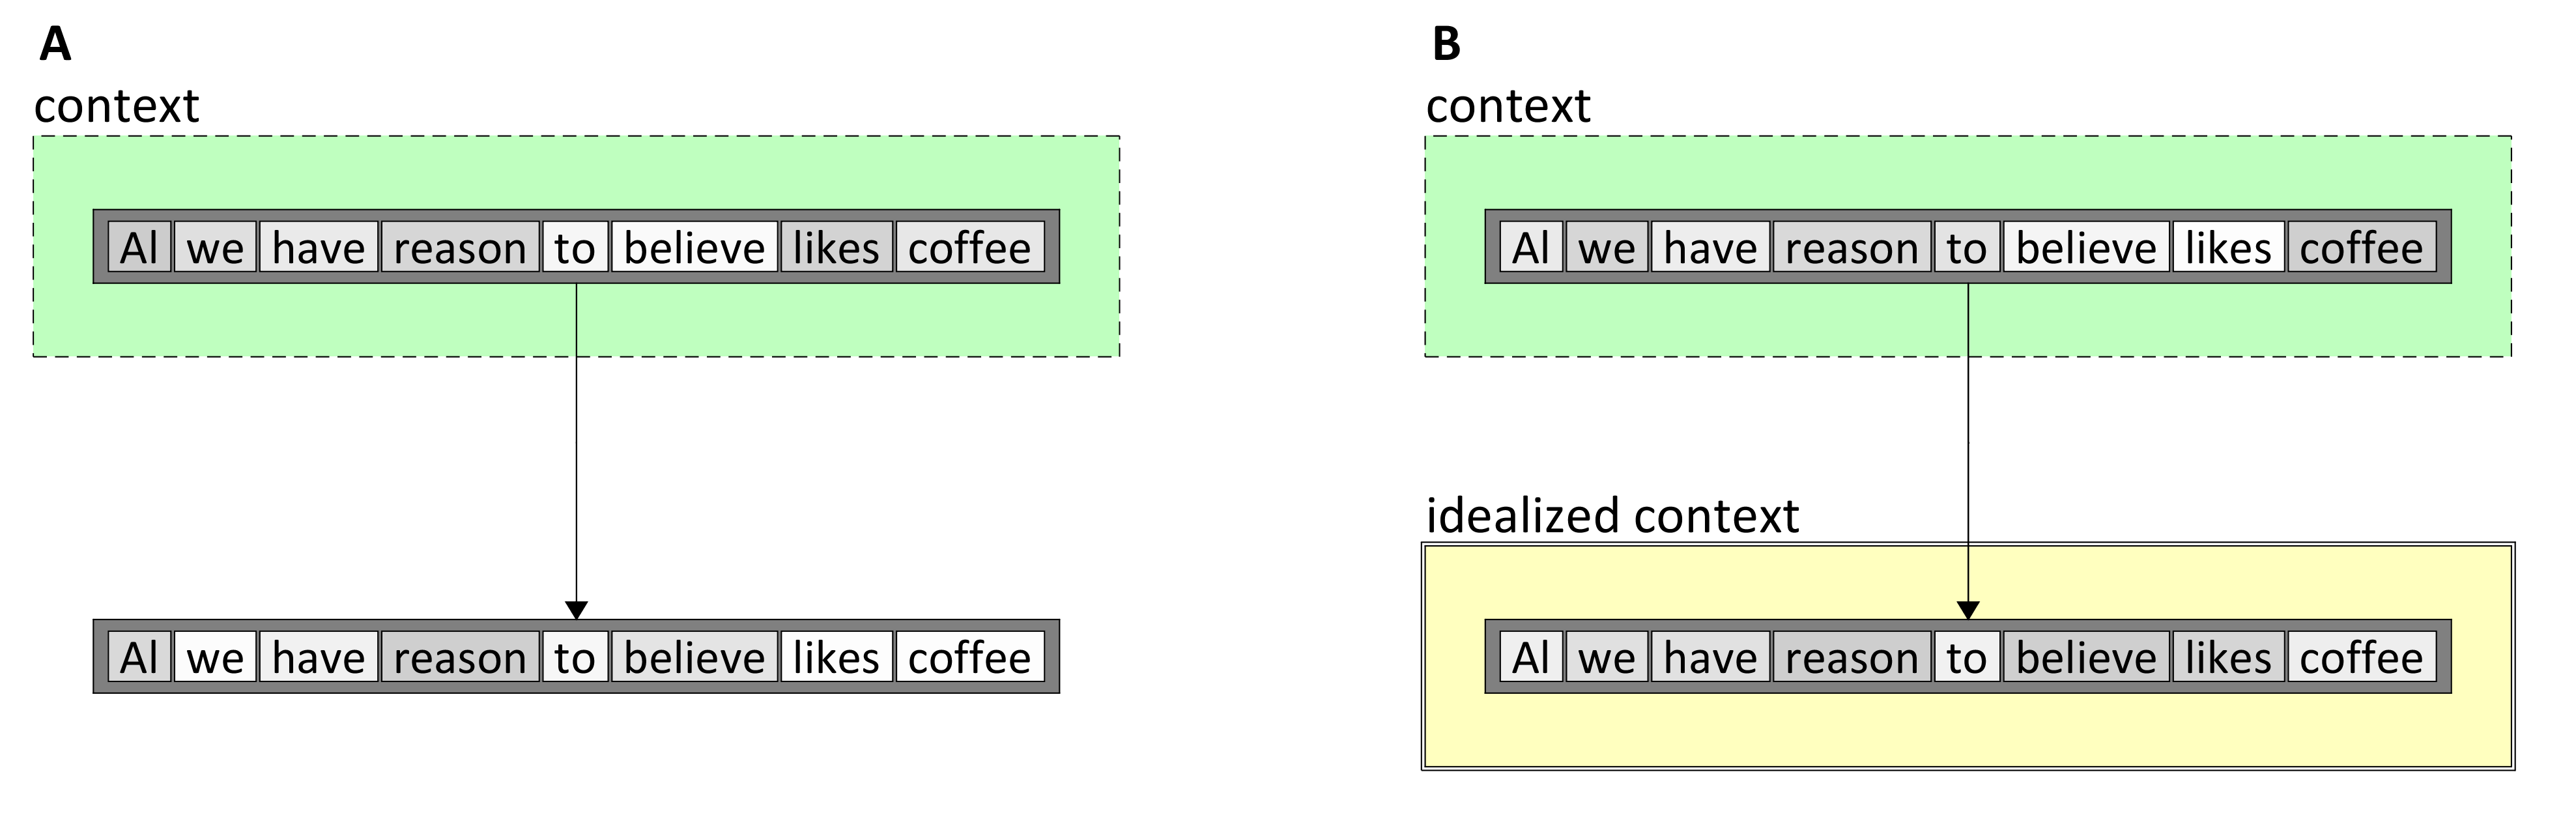
\includegraphics[width=\textwidth]{figures/Tilsen-img120.png}
\caption{A container schema is used for conceptualizing the relation between sentences and context.}
\label{fig:6:1}
\end{figure}
 

  The problem on both sides of the argument is the presupposition of the object/container metaphor, because it reifies the \isi{object metaphor} conception of language. From the o/el perspective, there is only a \isi{state space} with dimensions corresponding to system states, forces between systems, a \isi{surroundings}, and forces from the \isi{surroundings} -- the full system. All aspects of the full system are analytically imposed: we construct them ad hoc to suit our purposes. So, “where” is context in this conceptual model? Context is where we choose it to be. Some aspects of what is conventionally called \textit{context} are systems and corresponding dimensions of the \isi{state space}; other aspects of context -- the ones we choose to ignore or integrate -- become \isi{surroundings} and \isi{surroundings} forces. We are always free to reconstruct the analysis, reconceptualizing aspects of the \isi{surroundings} as systems, or reinterpreting systems as \isi{surroundings}. In other words, context is not a thing, nor a space for things, but rather the consequence of a choice regarding how to construct an analysis.

\subsection{Competence and performance: Objects and use of objects}

A big deal has been made of the distinction between competence and performance in relation to \isi{grammaticality} \citep{Chomsky1965}. The distinction is an early statement of the notion that there is some core implicit knowledge or mechanism, a narrow faculty of language, the essence of what language is. This core module is \textit{separate from} the \isi{sensorimotor} interfaces (note the spatial metaphor), which are to blame for deviations of actual production and comprehension from the idealized capacities of the core grammar (competence). In descriptions of the distinction, competence is described as \textit{knowledge}, while performance is not described as knowledge, but rather a “use” of knowledge. Hence the distinction constructs a difference in types: competence is the \textit{objects} themselves, performance is use of those objects:

\begin{quote}
We thus make a fundamental distinction between competence (the speaker-\isi{hearer}'s knowledge of his language) and performance (the actual use of language in concrete situations). \citep[4]{Chomsky1965}
\end{quote}


  From the o/el perspective, there is no such thing as “knowledge”, construed as objects. Instead, there are system states and \isi{surroundings}, a \isi{state space} and forces: there is no \textit{knowledge}, no \textit{objects}, no \textit{merge}. Knowledge and use are not distinguished, because knowledge is not a thing, nor a stuff. Instead, we imagine a multitude of microscopic dimensions, patterns of neural connectivity, neurotransmitter release, ion channels -- spatiotemporal order of enormously high dimension. Anything short of that is an analytical simplification; to call it knowledge (competence), and to dissociate it from observations of patterns in time, i.e. use of knowledge (performance), misleads us into believing that our categorization of “knowledge” is real. We should avoid misleading ourselves in this way.

\section{Grammatical coherence}

In the o/el framework, there is no conventional grammar on which \isi{grammaticality} intuitions could be based. A new conceptualization of intuitions is needed, one which helps us understand how intuitions emerge and evolve. The approach we take here is to view \isi{grammaticality}/\isi{acceptability} intuitions as the experience of \isi{coherence} or non-\isi{coherence} of system configurations in interpretation trajectories. For this purpose, we distinguish between \textit{grammatical coherence} and \textit{spectral coherence}. There are two varieties of \isi{spectral coherence}: auto-\isi{spectral coherence} applies to a single system, and cross-\isi{spectral coherence} applies to a pair of systems. These concepts are important for understanding the \isi{pre-stable phase} of interpretation. Spectral \isi{coherence} throughout an e-epoch is also a prerequisite for \isi{grammatical coherence}, which, as we explore below, is a consequence of whether in interpretation a stable \isi{reiterative trajectory} emerges.

For a reference point, we construct a canonical \isi{interpretation trajectory}, and then extend the canonical \isi{interpretation trajectory} to be \isi{reiterative}. We then apply the concept of \isi{coherence} on three scales: e-epochs, utterances, and discourse. One thing to emphasize at the outset of the analysis is that intuitions -- just like relational meanings -- are experiences which arise from system states. Thus any production or \isi{interpretation trajectory} is associated with some intuition(s), which may or may not be consciously recognized. We do not specifically address how people communicate their intuitions, or how intuitions induce action, although this is certainly a worthwhile line of inquiry.

\subsection{The canonical interpretation trajectory}

In the canonical \isi{interpretation trajectory} we assume a \isi{hearer} who hears an utterance produced by a \isi{speaker}. We impose a number of assumptions on this scenario:

First, the utterance conforms to a canonical \isi{production trajectory} and is coherent for the \isi{speaker}. This entails that for the \isi{speaker}, in the initial epoch of e-or\-ga\-ni\-za\-tion and in all subsequent epochs, the ϕ/e states of all excited systems are stationary and have a high degree of auto-\isi{coherence} and all cs-resonances have a high degree of cross-\isi{spectral coherence}. We also assume that if the \isi{speaker} and \isi{hearer} were interchanged, the \isi{interpreter} (who was the \isi{speaker} before the interchange) would experience a coherent \isi{interpretation trajectory}. 

Second, in the initial state no c-sys\-tems are excited. This lets us ignore “top-down” effects which would be manifested as \isi{surroundings} forces on systems. In more general interpretation trajectories these effects can be very important for determining \isi{coherence}.

Third, we assume that sensory systems (auditory and/or visual) associated with gm-sys\-tems from the utterance are veridically perceived by the \isi{interpreter}: excitation of those sensory systems unambiguously induces c-and s-sys\-tem excitations. Thus we ignore the possibility of ambiguities arising from multiple gm-domain to c-sys\-tem mappings (e.g. \textit{there’s a bathroom on the right} vs. \textit{there’s a bad moon on the rise}). Note that we generally have not incorporated sensory systems in our analyses; instead, we have left sensory systems as part of the \isi{surroundings}. Here we decide to construct sensory systems in the analysis, but we do not explicitly model their interactions with c-, s-, g-, and m-sys\-tems. Instead we stipulate their influences on the c- and s-sys\-tems that are our main focus.

Under the above assumptions, a canonical \isi{interpretation trajectory} of \textit{Al drinks coffee and tea} is shown below:

  
\begin{figure}
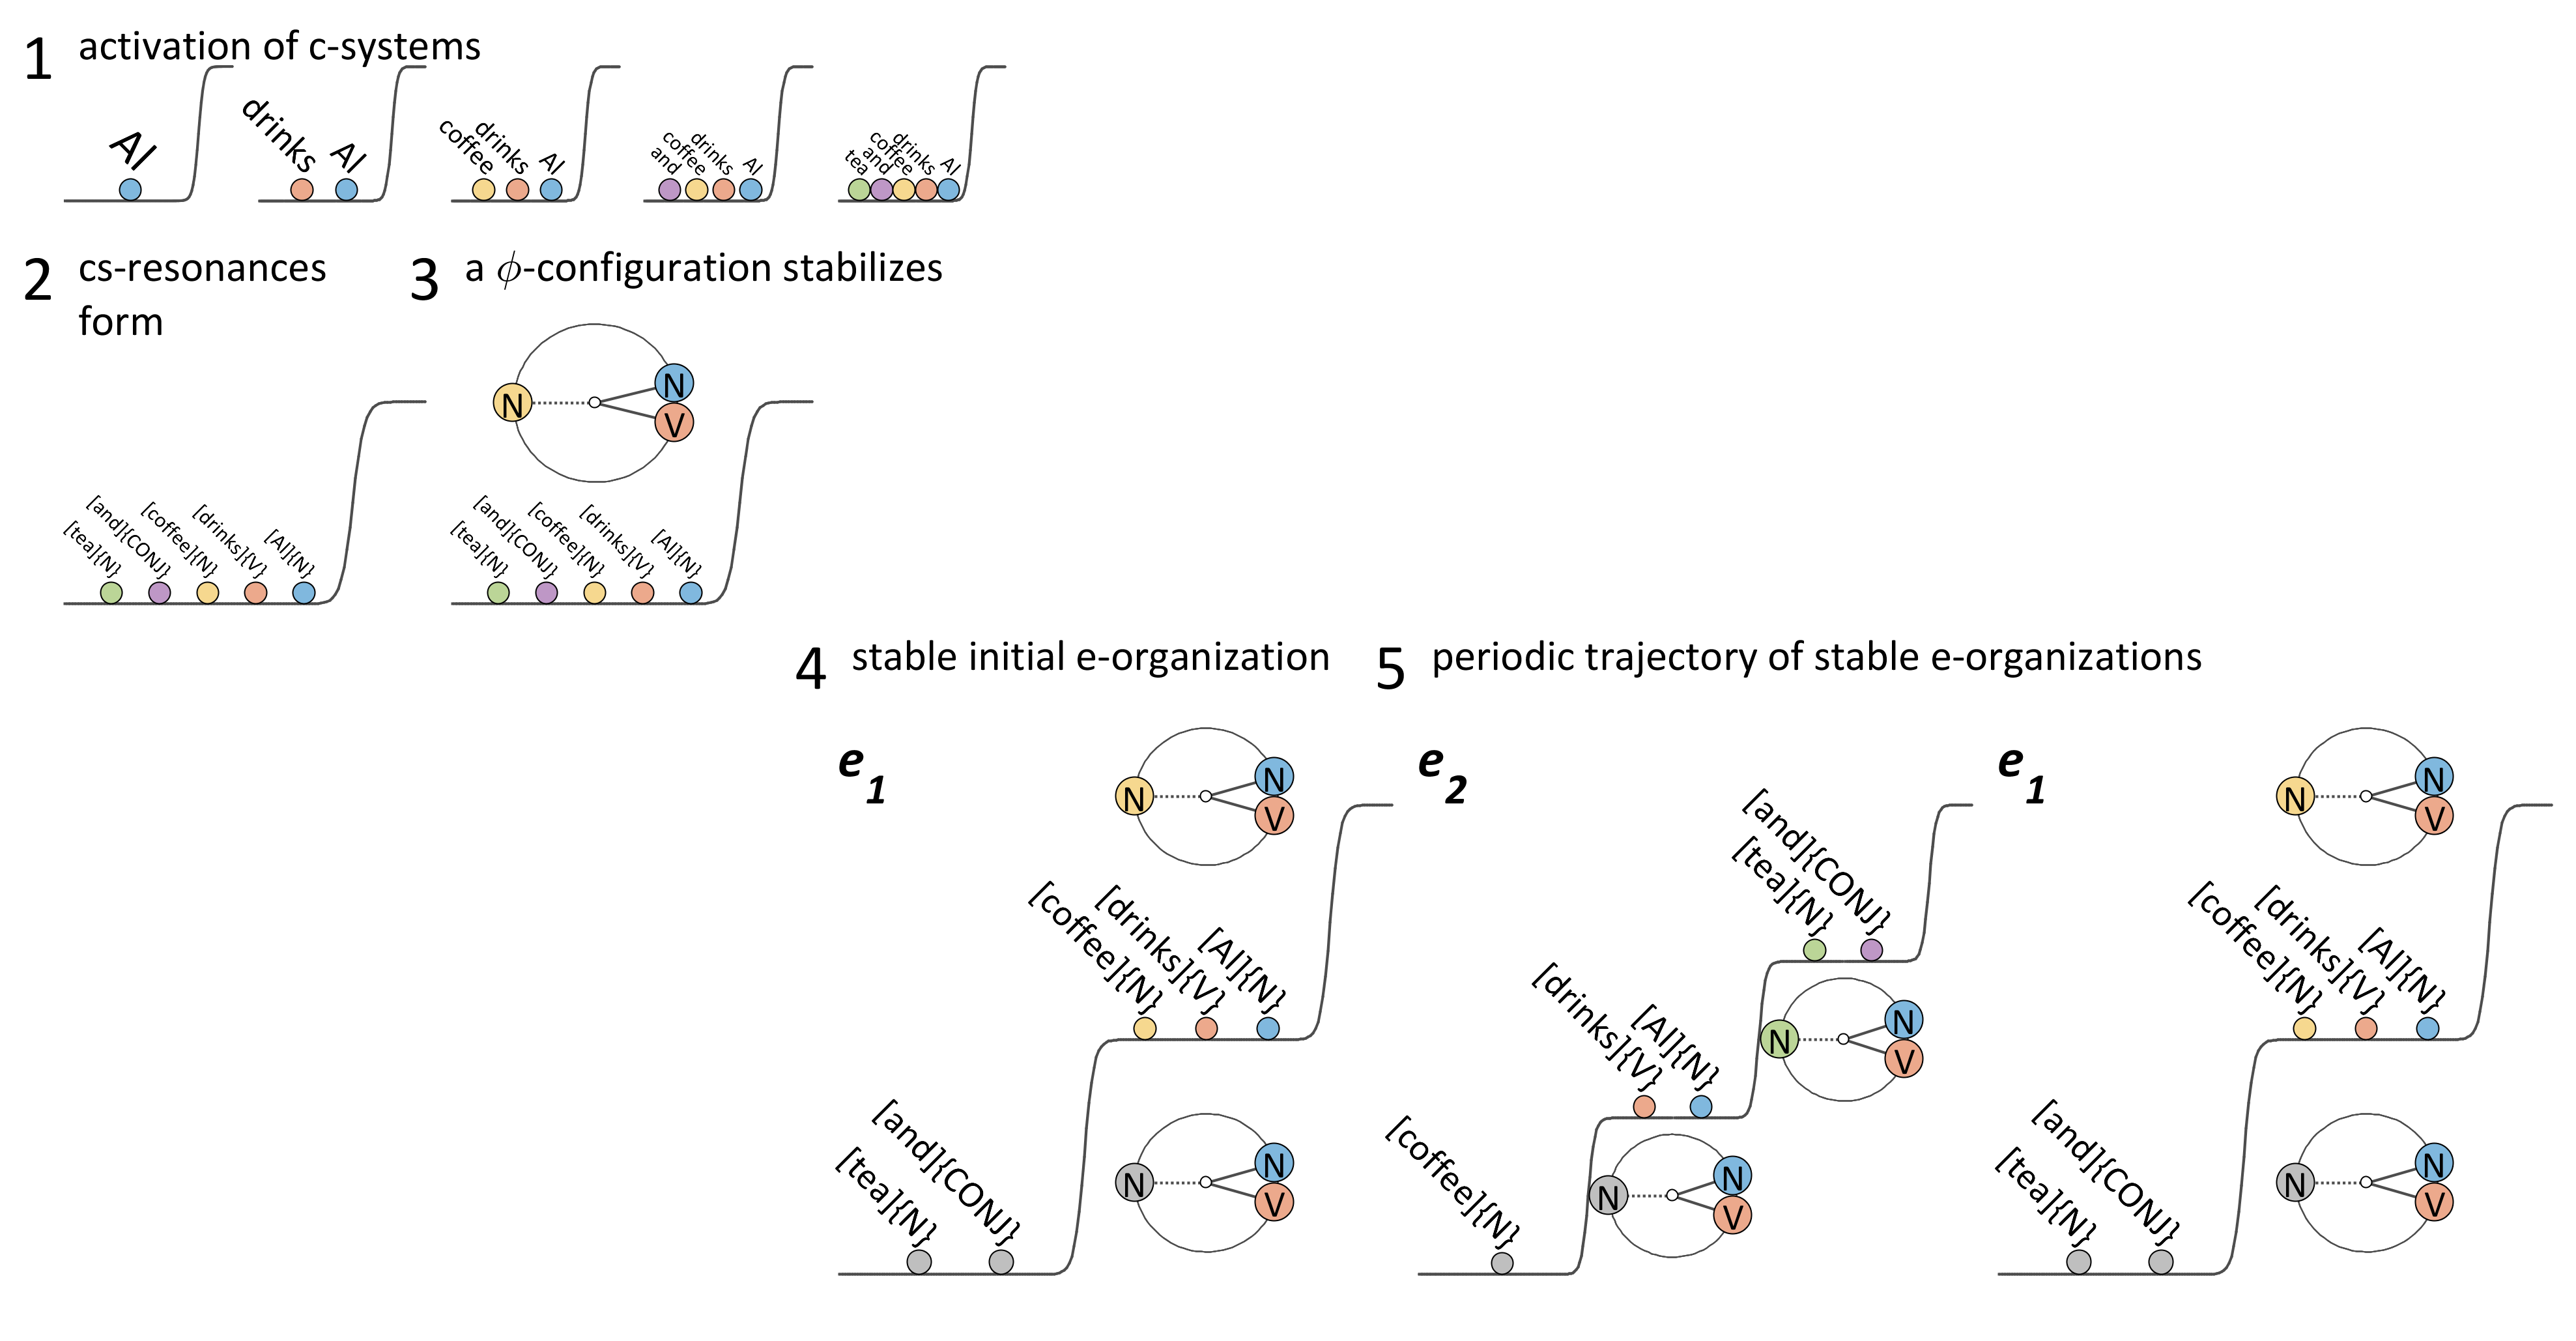
\includegraphics[width=\textwidth]{figures/Tilsen-img121.png}
\caption{Canonical interpretation trajectory of the utterance \textit{Al drinks coffee and tea}.}
\label{fig:6:2}
\end{figure}

\begin{enumerate}
\item[(1)]
The trajectory begins with a sequence of c-sys\-tem and s-sys\-tem excitations. In the canonical trajectory, only those c- and s-sys\-tems associated with the veridically perceived gm-sys\-tems in the utterance are excited. In general, \isi{surroundings} forces will influence the relative timing of when the relevant systems become excited, and some c-sys\-tems may already be excited from previous utterances or context, including ones which are not associated with the utterance. 
\item[(2)]
Each newly excited pair of c- and s-sys\-tems forms a cs-resonance. In the canonical trajectory, only the c-sys\-tems associated with the utterance couple to s-sys\-tems. In general, other c-sys\-tems may form cs-resonances, or may already be in resonant configurations with s-sys\-tems. Furthermore, the timing of when each cs-resonance forms is underdetermined. The activation of a cs-resonance resonance most likely begins shortly after the relevant sensory systems are activated, but may be further augmented by \isi{surroundings} forces.
\item[(3)]
Some ϕ-con\-fi\-gu\-ra\-tion stabilizes. \textit{Some} ϕ-con\-fi\-gu\-ra\-tion, but not necessarily all relevant ϕ-con\-fi\-gu\-ra\-tions. The stabilization process begins when cs-sys\-tems emerge in the previous stage, and the timecourse of cs-sys\-tem emergence may influence which ϕ-con\-fi\-gu\-ra\-tion stabilizes first. No particular ϕ-con\-fi\-gu\-ra\-tion must stabilize first, although we assume that earlier activation of a configuration makes earlier stabilization more likely -- in other words, parsing is incremental. 
\item[(4)]
A stable initial e-or\-ga\-ni\-za\-tion arises. In the canonical scenario, the excited systems are those associated with the ϕ-con\-fi\-gu\-ra\-tion which stabilized first. In general e-or\-ga\-ni\-za\-tion can begin before ϕ-stabilization, but e-stabilization must follow the stabilization of a ϕ-con\-fi\-gu\-ra\-tion (this is a consequence of our hypothesis that ϕ-or\-ga\-ni\-za\-tion can influence e-or\-ga\-ni\-za\-tion). 
\item[(5)]
The canonical \isi{interpretation trajectory} leads to a state in which a \isi{reiterative trajectory} can occur. In the above example, the sequence of epochs (e1…e2) is reiterated, i.e. an alternation between configurations in which {\textbar}Al drinks coffee{\textbar} is attended, and configurations in which {\textbar}Al drinks tea{\textbar} is attended. To distinguish \isi{canonical interpretation} from canonical production, we analyze the \isi{interpretation trajectory} as a non-simulative (s-gated and m-gated) regime. In general interpretation trajectories we can relax this assumption and allow for cs-simulation (an m-gated trajectory) or gm-simulation (an exec-gated trajectory).
\end{enumerate}

  Reiterative trajectories play an important role in interpretation. Reiteration allows for a trajectory that emerges in interpretation to be less dependent on initial conditions and less dependent on the timecourse of system activation. It also provides a mechanism whereby relatively complex utterances which may be initially unstable can become coherent. Recall that a \isi{reiteration} is a sequence of unique stable states e\textsubscript{i} … e\textsubscript{n} where e\textsubscript{n} = e\textsubscript{i}. In other words, the system trajectory cycles through a sequence of states. Reiteration is a reconceptualization of “working memory” for \isi{relational meaning} experiences. An example \isi{reiteration} of \textit{Bo knows Al drinks coffee} is shown in {\figref{fig:6:8}}. After an initial unstable epoch (e0), there is a stable state (e1) in which {\textbar}Bo knows{\textbar} is attended and {\textbar}Al drinks coffee{\textbar} is grounded, then a transition to (e2) in which {\textbar}Al drinks coffee{\textbar} is attended and {\textbar}Bo knows{\textbar} is grounded. This is followed by a transition to (e′\textsubscript{1}), which is equivalent to e1. Hence the trajectory is \isi{reiterative}.

  
\begin{figure}
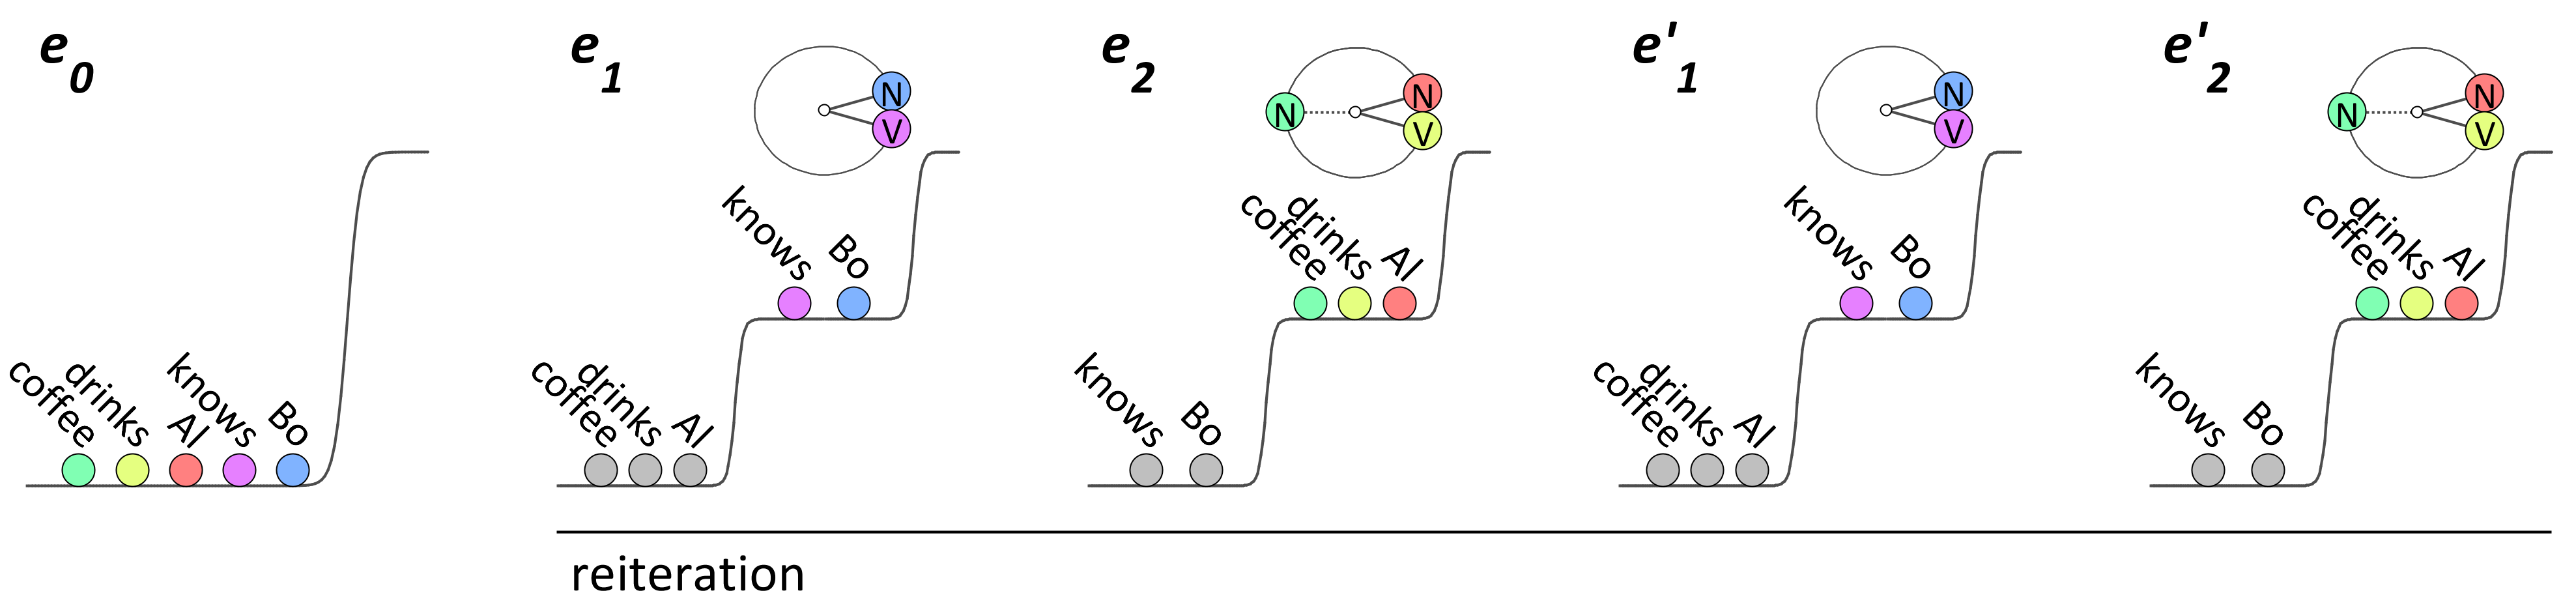
\includegraphics[width=\textwidth]{figures/Tilsen-img122.png}
\caption{A reiterative trajectory arises in interpretation.}
\label{fig:6:3}
\end{figure}
 

  We remain agnostic regarding whether reorganizations in \isi{reiterative} trajectories typically occur with cs-selection. This is represented in the potentials above by the empty \isi{selection level}, and we refer to such trajectories as non-selectional, or s-gated. Alternative possibilities are that \isi{reiteration} is cs-simulative, i.e. the trajectory involves selection of cs-sys\-tems without gm-selection, or the \isi{reiteration} is gm-simulative, with closed execution gates. It is unclear whether our analyses of \isi{coherence} hinge on this difference in regime, although we suspect that interpreters are not aware of non-selectional \isi{reiteration} to the same degree that they are aware of cs-selectional \isi{reiteration}.  

  The applicability of \isi{reiteration} is not restricted to attention-switching between entire clauses. Any sequence of stable configurations can be reiterated. What makes \isi{reiteration} important is its function as a stabilization mechanism with mnemonic advantages. An example of a \isi{reiterative trajectory} is shown in {\figref{fig:6:4}}.  

\ea{Al drinks coffee and tea, and eats granola and eggs.}
\z
  
\begin{figure}
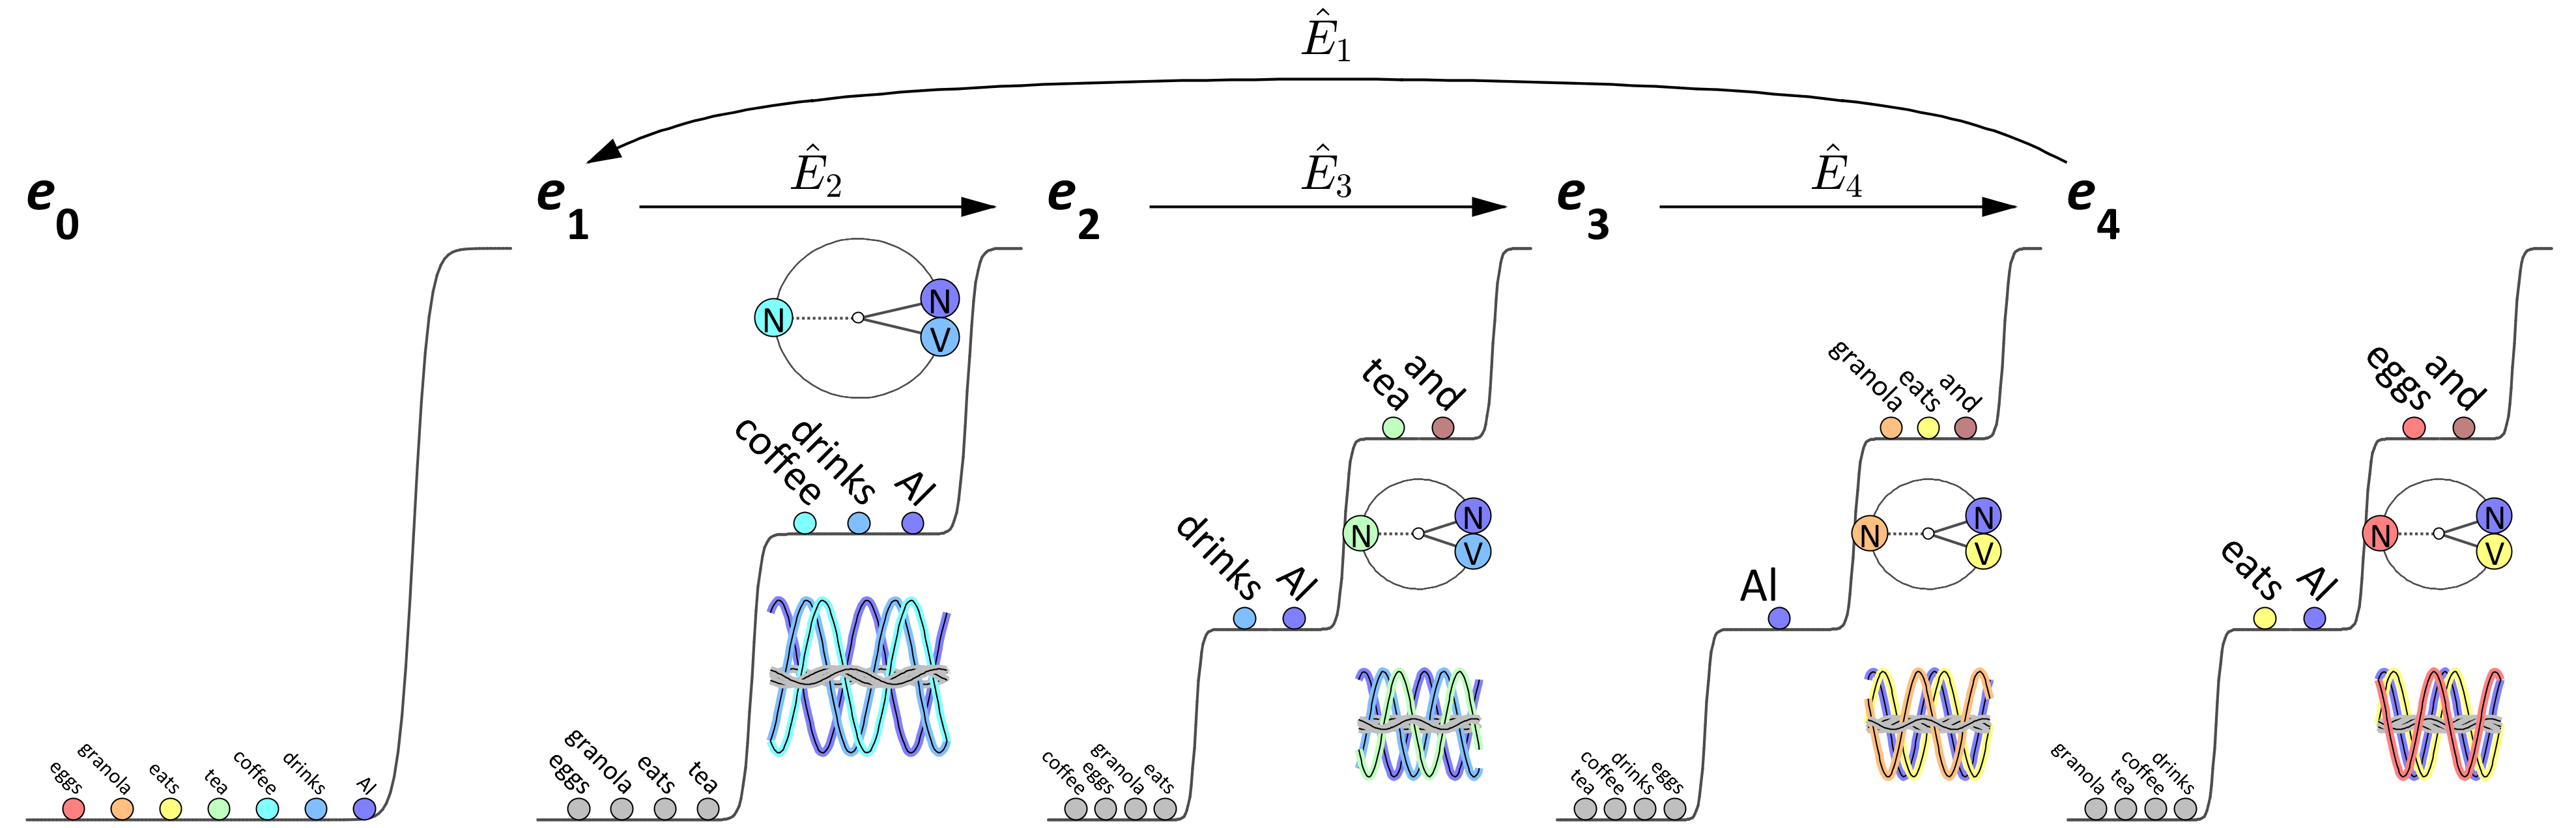
\includegraphics[width=\textwidth]{figures/Tilsen-img123.png}
\caption{Reiterative trajectory involving four ϕ-con\-fi\-gu\-ra\-tions.}
\label{fig:6:4}
\end{figure}
 

  Interpretation of this utterance involves a \isi{reiterative} sequence of four ϕ-con\-fi\-gu\-ra\-tions. In each epoch of the \isi{reiteration} (e1--e4), a different subset of cs-sys\-tems is above ground, while others are grounded. Because there are multiple cs-sys\-tems of the same \isi{syntactic category}, there is a potential for differentiation \isi{interference}. The grounding of unattended systems mitigates against this \isi{interference}. However, this comes at a cost: reorganization operations must be selective rather than canonical, i.e. the analysis requires ungrounding promotions and grounding demotions. For example, Ê\textsubscript{2} selectively demotes [coffee] to ground and promotes [tea] from ground; Ê\textsubscript{3} demotes [drinks] and [tea] while promoting [eats] and [granola]. Note that we analyze [and]\{CONJ\} as a system which is excited to \isi{selection level} with each \isi{ungrounding promotion}, just as in production trajectories.

  The above mechanism generalizes to arbitrarily long utterances, as in \textit{Al drinks coffee and tea, and eats granola and eggs, and Bo drinks whisky and beer, and eats porridge and salad}. How can an \isi{interpreter} remember the complicated sequence of reorganizations which are required for attending to all of the relational meanings in such an utterance? Of course, an \isi{interpreter} might not successfully remember such a sequence. But it is possible; and most people would require some practice. We conjecture that \isi{reiteration} is the mechanism of this “practice” and induces “learning”, i.e. microscale changes which constitute a form of “long-term memory” for the sequence of non-canonical reorganizations. Reiteration with cs-selection, gm-selection, and execution are probably even more effective in this regard: overt execution is the most effective mnemonic technique, \isi{subvocal rehearsal} (exec-gated production) the next most effective, and m-gated cs-simulation the least effective.

  The hypothesized learning which \isi{reiteration} facilitates can be viewed as learning of a sequence of e-reorganizations, which determines an e-space trajectory. There are interesting questions regarding the timescales on which such changes persist, which relate to distinctions between scales of memory (working, short-term, and long-term). The question of how we can learn to remember long sequences warrants further investigation. What is essential here, is that, on the utterance timescale, we do not need to impose any new organizing mechanism for \isi{relational meaning} experiences. 

\subsection{Grammatical coherence: scales and criteria}

The concept of \isi{grammatical coherence} can be applied on three scales: the smallest scale involves an e-epoch in which at least one but no more than a few ϕ-con\-fi\-gu\-ra\-tions are continuously attended. On this epochal scale, \isi{coherence} only requires that all above-ground cs-sys\-tems participate in some stable set of ϕ-con\-fi\-gu\-ra\-tions. This entails that the cross-\isi{spectral coherence} for any pair of systems will be relatively high, because frequency-locking is required for stability. We can also apply \isi{grammatical coherence} to the interpretation of an entire utterance; on the utterance scale, \isi{grammatical coherence} requires epochal \isi{coherence} for all epochs in the utterance, as well as a potential for a \isi{reiterative simulation} of the trajectory. The most relevant scale for analysis of \isi{grammaticality}/\isi{acceptability} intuitions is the discourse scale, on which \isi{coherence} requires \isi{utterance coherence} and the condition that the attended ϕ-con\-fi\-gu\-ra\-tions of the \isi{interpreter} correspond to the attended ϕ-con\-fi\-gu\-ra\-tions of the producer. Note that we do not require that the sequence of \isi{interpreter} e-epochs be the same as those of the producer. Hence the following criteria give rise to a \isi{grammatical coherence} hierarchy:

\begin{itemize}
\item[i.] 
All excited cs-sys\-tems participate in some stable, coherent set of ϕ-con\-fi\-gu\-ra\-tions.
\item[ii.] 
A sequence of stable, coherent ϕ-con\-fi\-gu\-ra\-tions can be reiterated.
\item[iii.] 
Each ϕ-con\-fi\-gu\-ra\-tion in the potentially \isi{reiterative} \isi{interpretation trajectory} corresponds to a ϕ-con\-fi\-gu\-ra\-tion in an associated \isi{production trajectory}.
\end{itemize}

\begin{table}
\begin{tabularx}{.66\textwidth}{rCCC}
\lsptoprule
& (i) & (ii) & (iii)\\
\midrule 
\raggedleft \isi{epoch coherence} & y &  & \\
\raggedleft \isi{utterance coherence} & y & y & \\
\raggedleft \isi{discourse coherence} & y & y & y\\
\lspbottomrule
\end{tabularx}
\caption{The grammatical coherence hierarchy.}\label{tab:6:1}
\end{table}
  The \isi{epoch coherence} criterion is that all of the above-ground systems in an e-epoch must participate in at least one stable ϕ-con\-fi\-gu\-ra\-tion. The states in {\figref{fig:6:5}}(A--D) below fail to meet this criterion. In (A), imagine that an \isi{interpreter} hears the name \textit{Al}. Without any other cs-sys\-tem to couple with, [Al]\{N\} does not participate in a stable ϕ-con\-fi\-gu\-ra\-tion. When an unstable state such as (A) arises, we can anticipate two possible continuations of the trajectory. In one, [Al]\{N\} becomes grounded; in the other, additional cs-resonances become excited and a coherent configuration stabilizes. Many pragmatic phenomena can be understood as trajectories in which an utterance evokes an unstable configuration which evolves to a stable configuration when other cs-sys\-tems become excited. Often we can construct analyses in which other systems are excited for contextual reasons. Consider the utterance \textit{Al coffee} in (B); excitation of these two cs-sys\-tems in unstable. However, if we imagine that [drink]\{V\} is also above-ground because the producer and \isi{interpreter} are discussing who drinks what (e.g. \textit{Al coffee, Bo tea, Cam whisky, Dee beer…}), then the \isi{epoch coherence} criterion would be met.

  
\begin{figure}
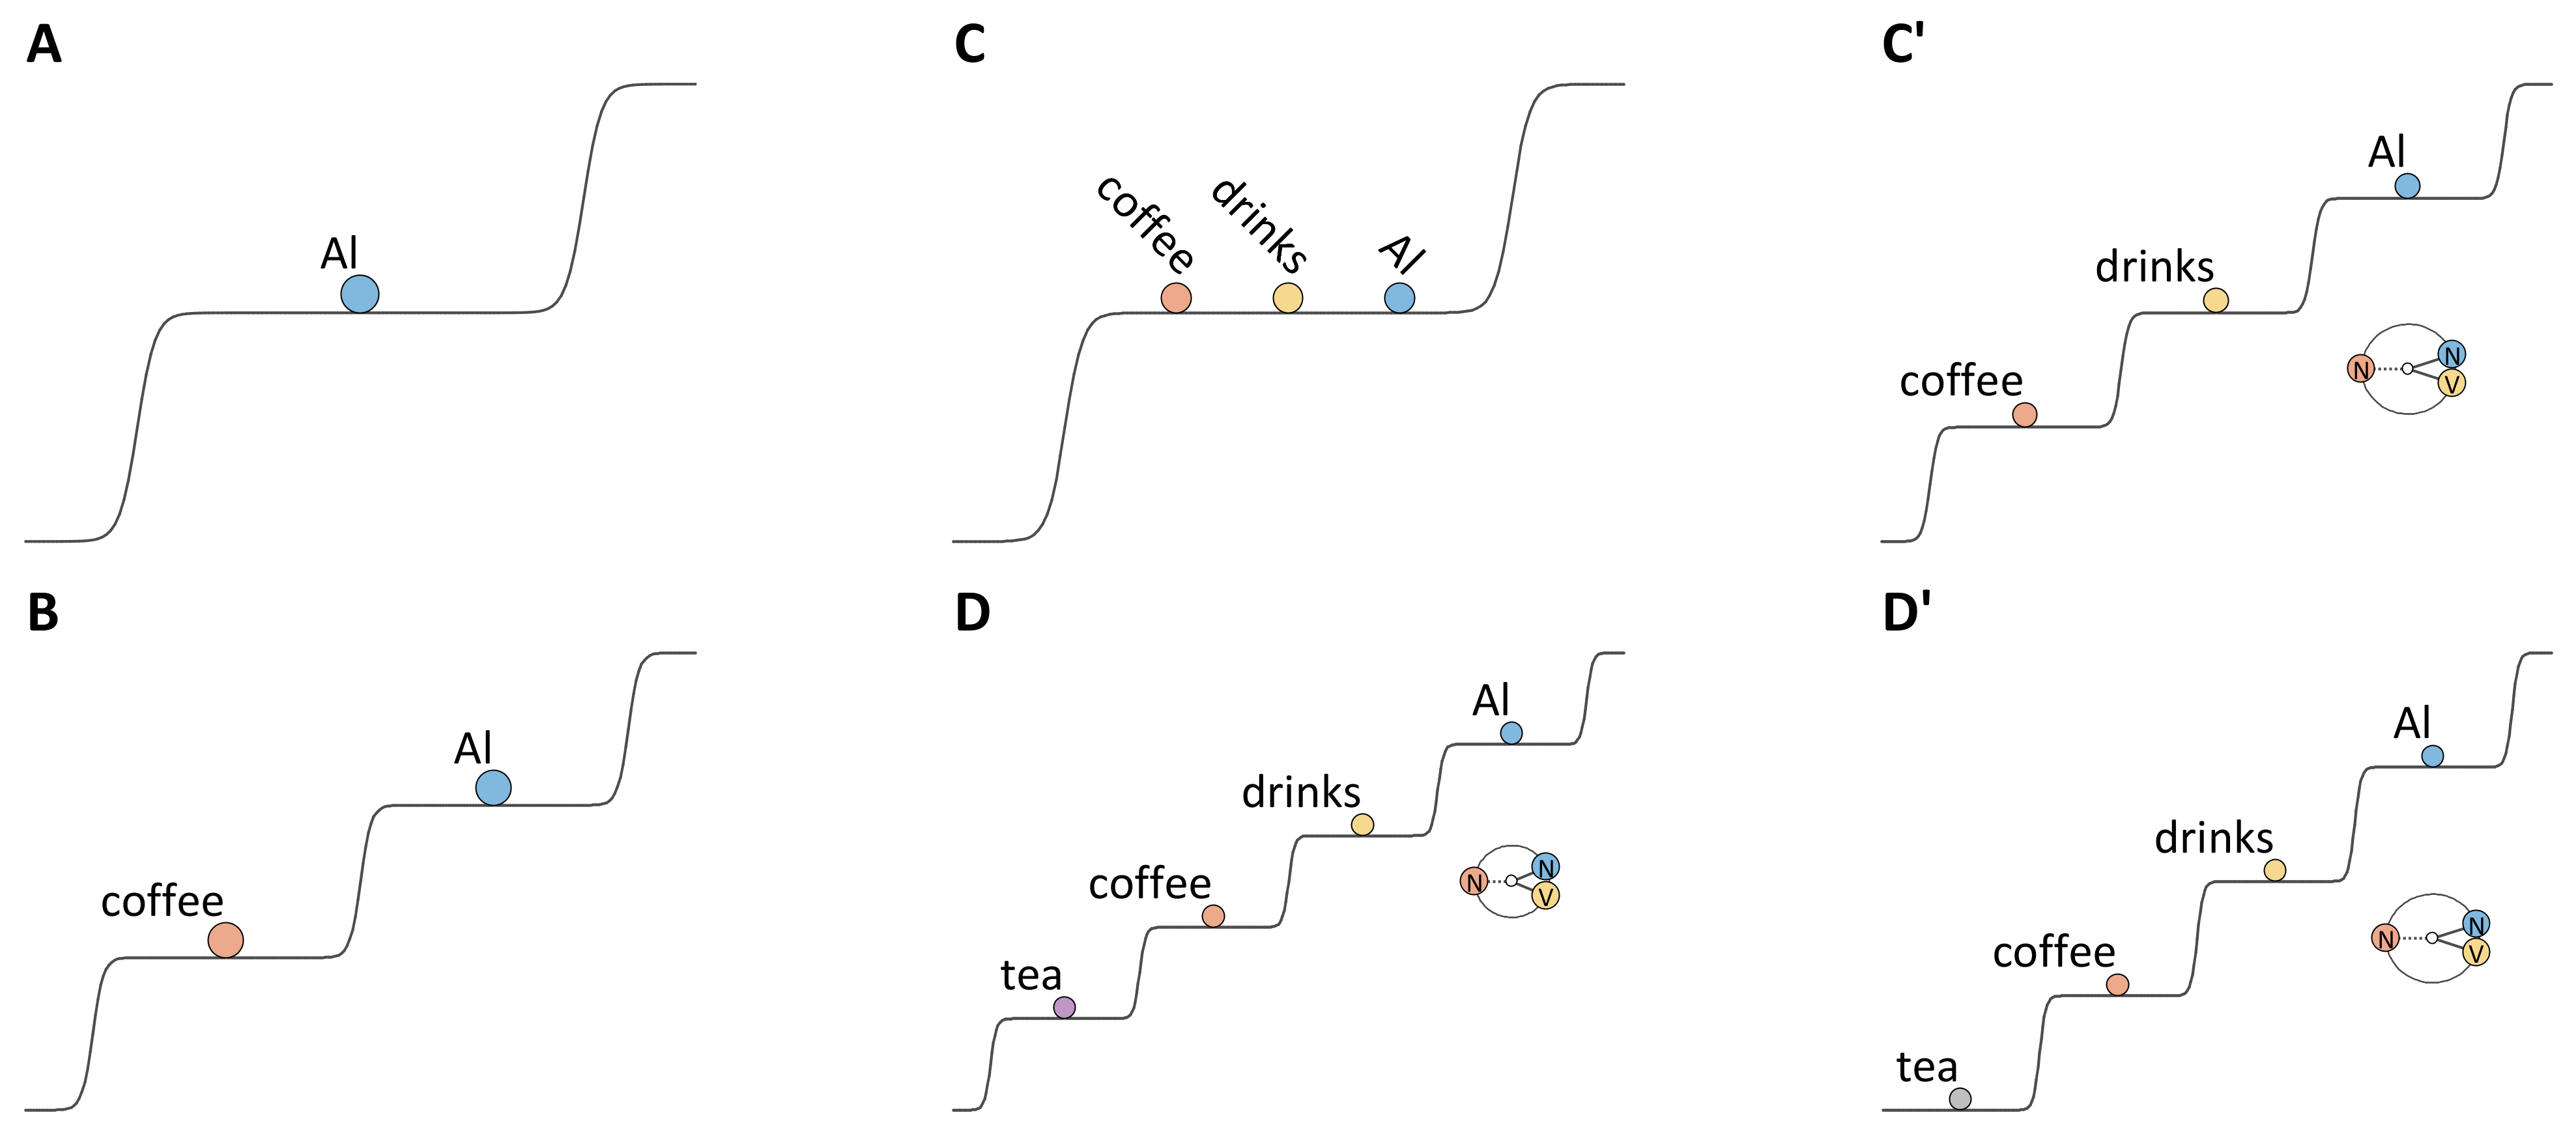
\includegraphics[width=\textwidth]{figures/Tilsen-img124.png}
\caption{Examples of non-coherent epochs. The configurations in C$'$ and D$'$ are coherent versions of the configurations in C and D.}
\label{fig:6:5}
\end{figure}
 

  In (C) we imagine that an \isi{interpreter} hears \textit{Al drinks coffee}, and that all cs-sys\-tems are above-ground but occupy the same e-level. Because there is no stable ϕ-con\-fi\-gu\-ra\-tion, the state is non-coherent. However, we do not know whether or not a stable ϕ-con\-fi\-gu\-ra\-tion \textit{could} evolve from the e configuration in (C), and so it is not the e-or\-ga\-ni\-za\-tion which makes the configuration unstable, but rather, the absence of a stable ϕ-con\-fi\-gu\-ra\-tion. In the absence of other forces, we expect that a reorganization to the coherent state in (C$'$) occurs in conjunction with the emergence of stable ϕ and e-con\-fi\-gu\-ra\-tions. This example illustrates that \isi{coherence} derives from a system state, and does not depend on the path taken to arrive at that system state (of course, many paths may not lead to \isi{coherence}). 

  Example (D) is non-coherent because [tea]\{−N\} is above-ground but does not participate in a stable ϕ-con\-fi\-gu\-ra\-tion. We note that the underlying cause of the instability is differentiation \isi{interference}: \{−N\} cannot differentiate into stable [tea]\{−N\} and [coffee]\{−N\} cs-resonances in this configuration. The instability in (D) is typically resolved by grounding the less highly excited system as in (D$'$). Indeed, we note that the grounding from (D) to (D$'$) is not necessarily a distinct mechanism from the one which governs e-or\-ga\-ni\-za\-tion in early production: cs-resonances compete for excitation.

The \isi{utterance coherence} criterion specifies that there is a \textit{potentially} periodic sequence of epochs (i.e. \isi{reiterative trajectory}), each of which meets the epochal \isi{coherence criterion}. It is not required that all epochs which arise in the interpretation of an utterance are coherent, only that an uninterrupted sequence of epochs occurs, through the same re-or\-ga\-ni\-za\-tion operations which are available for production. It is also not required that the sequence \textit{actually} repeats. We only require that the \isi{interpreter} system evolves to a state from which re-or\-ga\-ni\-za\-tion can return the system to the first state in the sequence. Consider an utterance with a parenthetical, such as \textit{Al, Bo knows, drinks coffee}, shown in {\figref{fig:6:6}}.\footnote{Note that for the sake of providing more compact representations of trajectories which involve multiple ϕ-epochs, we sometimes represent excited systems on the same e-level, but we nonetheless imagine those systems to occupy distinct e-levels. Note also that we do not require that any systems have selection-level excitation, and therefore canonical reorganizations are unnecessary; thus only selective reorganizations are shown in this figure.}

\begin{figure}
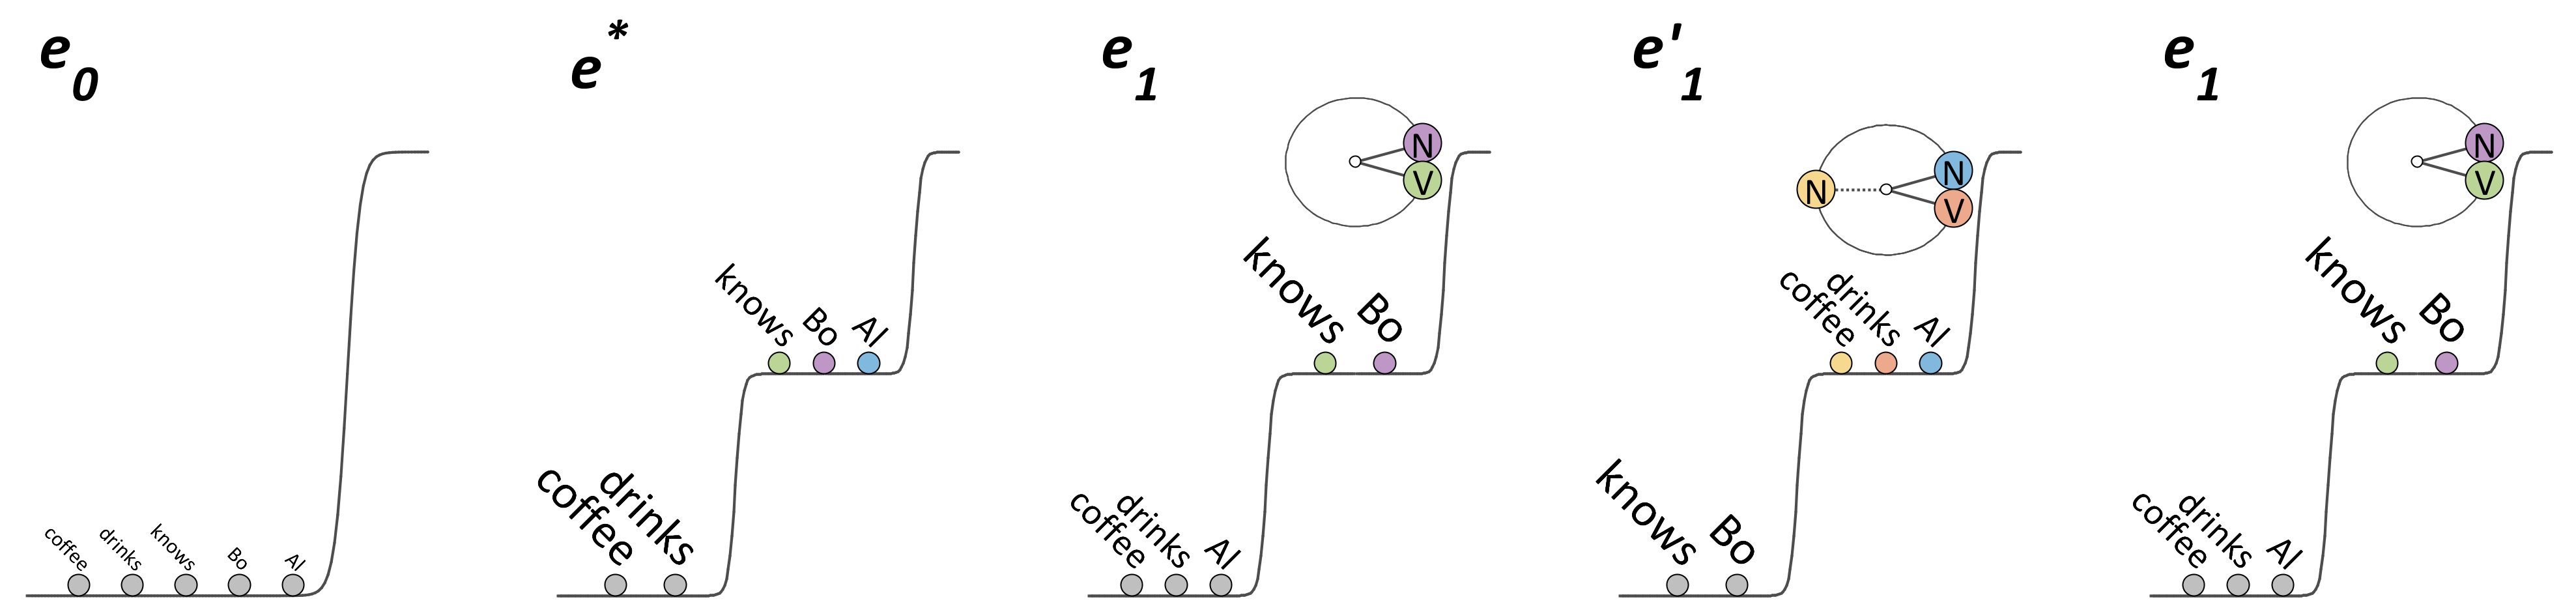
\includegraphics[width=\textwidth]{figures/Tilsen-img125.png}
\caption{Utterance coherence is achived when a trajectory of coherent epochs can be reiterated.}
\label{fig:6:6}
\end{figure}
 
  For \isi{utterance coherence}, a potentially periodic trajectory of individually coherent epochs must occur for the \isi{interpreter}. In epoch (e*), a non-coherent state, \isi{coherence} has not been achieved. However, if subsequently the trajectory (e\textsubscript{1}), (e$′$\textsubscript{1}) arises, then \isi{coherence} is achieved: (e$′$\textsubscript{1}) can evolve to (e\textsubscript{1}) through \isi{selective reorganization}, and vice versa, in effect shifting attention between two ϕ-con\-fi\-gu\-ra\-tions. Note that the reorganization from (e*) to (e1) involves a \isi{grounding demotion} of [Al]\{N\}, which would be the first active cs-sys\-tem in the canonical trajectory. In the above example, the \isi{reiteration} that arises does not necessarily match the initial e-or\-ga\-ni\-za\-tion of the producer, nor does it match the trajectory which occurred for the producer during execution.

  As with \isi{epoch coherence}, the \isi{interpretation trajectory} that leads to an ut\-ter\-ance-coherent trajectory is not relevant to assessment of \isi{coherence}: a trajectory in which non-coherent states such as (e*) in {\figref{fig:6:6}} occur before the potentially \isi{reiterative trajectory}. However, \isi{coherence} intuitions may derive not only from whether a coherent trajectory is ultimately achieved, but also from experience of incoherent states prior to \isi{coherence}. Thus we should think of \isi{utterance coherence} intuitions as determined by a trajectory of experiences of states.

  Because \isi{utterance coherence} does not require any correspondence between producer and \isi{interpreter} states, it is not very useful for conceptualizing \isi{grammaticality} intuitions relative to a producer trajectory. Indeed, \isi{utterance coherence} occurs when the \isi{interpreter} reaches any coherent \isi{reiterative trajectory}, regardless of what the producer intended. Thus from the initial state in (e\textsubscript{0}) below, where we assume the \isi{speaker} intended {\textbar}Bo knows{\textbar} and {\textbar}Al drinks coffee{\textbar} configurations, if the \isi{interpreter} attends to {\textbar}Al knows{\textbar} and {\textbar}Bo drinks coffee{\textbar} configurations in state (e1) and state (e2), \isi{coherence} is achieved, despite the producer-\isi{interpreter} mismatch in ϕ-con\-fi\-gu\-ra\-tions.

  
\begin{figure}
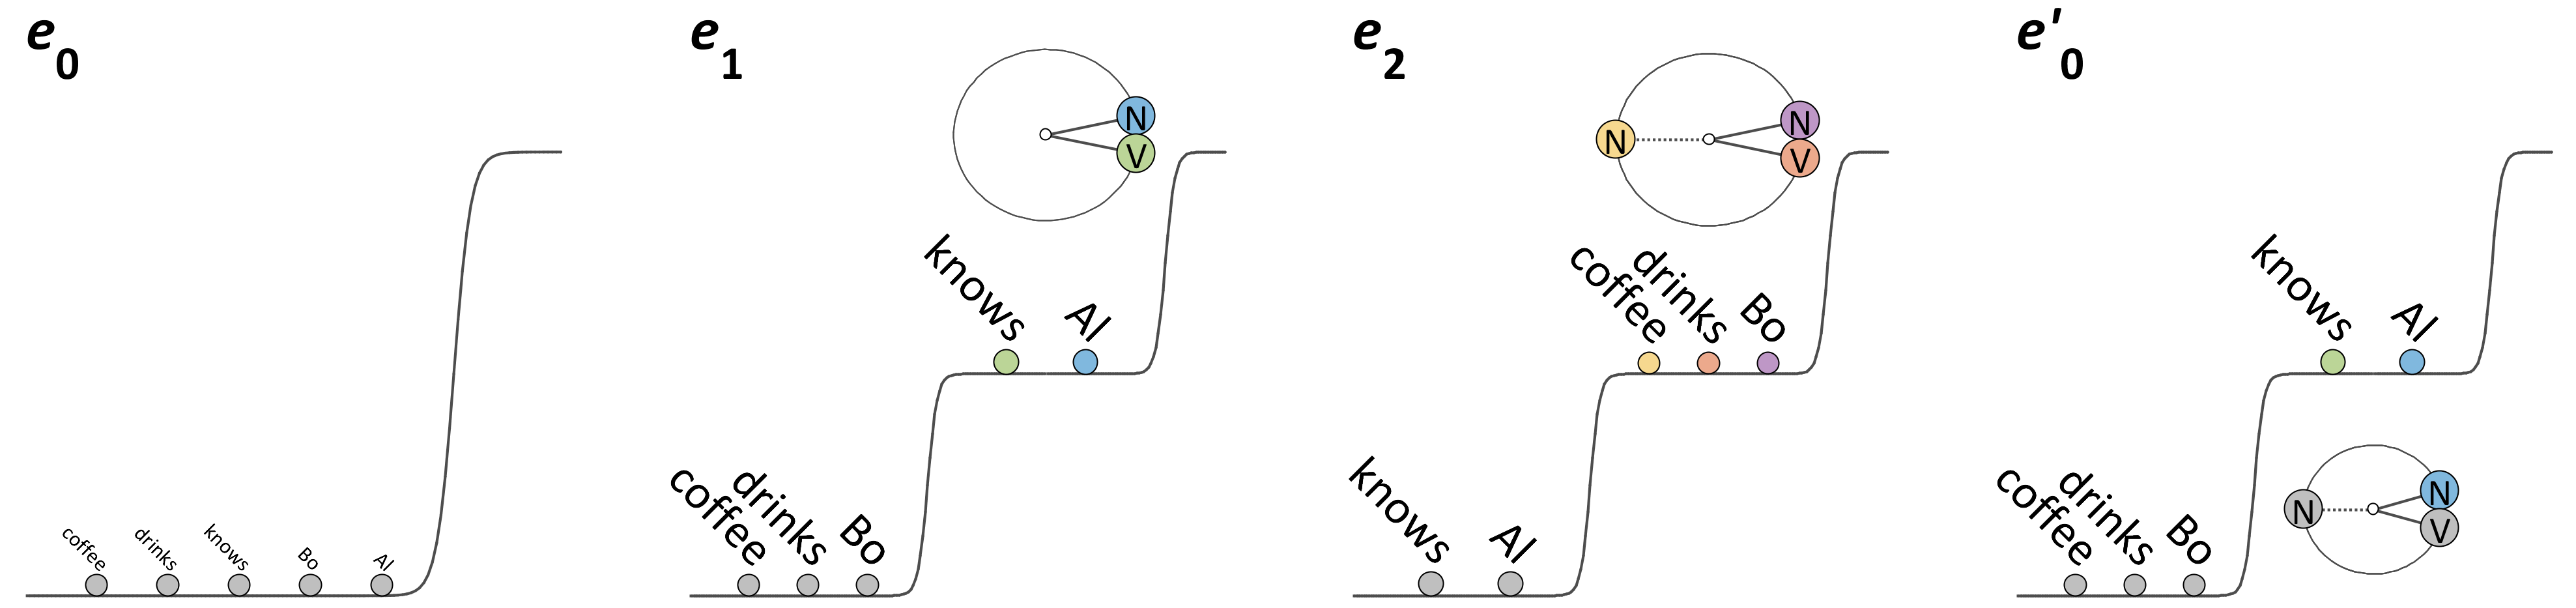
\includegraphics[width=\textwidth]{figures/Tilsen-img126.png}
\caption{Utterance coherent interpretation trajectory which does not correspond to the producer trajectory.}
\label{fig:6:7}
\end{figure}
 

  It is important to emphasize that we cannot precisely say “an utterance is coherent”, because \isi{coherence} is not a property of utterances. Utterance \isi{coherence} is \isi{coherence} associated with the timescale of utterances, which can span multiple epochs of attention. We can only say that a coherent, potentially \isi{reiterative trajectory} occurs in the interpretation of an utterance. Moreover, this does not imply that the trajectory remains coherent: reorganizations might occur, for a number of reasons, which prevent the trajectory from being potentially reiterated.

  Discourse \isi{coherence} requires the additional condition that ϕ-con\-fi\-gu\-ra\-tions in the \isi{interpreter} \isi{reiteration} correspond to ones that arose during the cs-/gm-selective phase of a \isi{production trajectory}. Thus unlike epoch and \isi{utterance coherence}, \isi{discourse coherence} requires consideration of both \isi{interpreter} and producer trajectories. Specifically, for each excited ϕ-con\-fi\-gu\-ra\-tion in the \isi{selectional regime} of a \isi{production trajectory}, that same ϕ-con\-fi\-gu\-ra\-tion arises in the \isi{interpretation trajectory}. Only ϕ-con\-fi\-gu\-ra\-tions which are excited in selectional epochs of the \isi{production trajectory} are relevant to \isi{discourse coherence}, because it is possible for a noncanonical \isi{production trajectory} to visit arbitrary states before and after the states which govern cs-sys\-tem selection. 

  One important aspect of the correspondence criterion for \isi{discourse coherence} is that the specific sequence of ϕ-con\-fi\-gu\-ra\-tions an \isi{interpreter} experiences need not match the specific sequence of ϕ-con\-fi\-gu\-ra\-tions which a producer experiences. Imposing this condition results in a stricter version of \isi{discourse coherence}, but may be hard to apply because producer e-state trajectories can be highly underdetermined for relatively complicated utterances. One possible solution to this problem is to require ϕ/e \isi{reiteration} correspondence between producer and \isi{interpreter}, but this requires us to stipulate that a \isi{reiterative} producer trajectory always occurs, which is far from obvious.

  Another issue with the \isi{discourse coherence} criterion is that we have no well-defined notion of “the same” cs-sys\-tem between a producer and \isi{interpreter}, at least not when the producer and \isi{interpreter} are different people. We can ignore this problem or circumvent it by imagining that the \isi{interpreter} and producer are the same person. This is the case for self-reflective \isi{grammaticality}/\isi{acceptability} intuitions that are often used in syntactic theory construction. However, in the more general situation where producer and \isi{interpreter} are not the same person, the concept of \isi{discourse coherence} requires further assumptions regarding similarity of cs-sys\-tems between different individuals.  

\subsection{Incremental organization in interpretation}

How does a stable configuration first arise in interpretation? In the canonical \isi{interpretation trajectory}, sensory systems exert forces on c-sys\-tems and s-sys\-tems, which activate them and induce cs-resonances. The canonical trajectory makes the assumption that all cs-resonances were in an active, unexcited state before ϕ/e organization occurs, as in the trajectories below. But this oversimplification is obviously empirically inadequate. In most cases we expect some organization to arise before production of an utterance has finished.

  
\begin{figure}
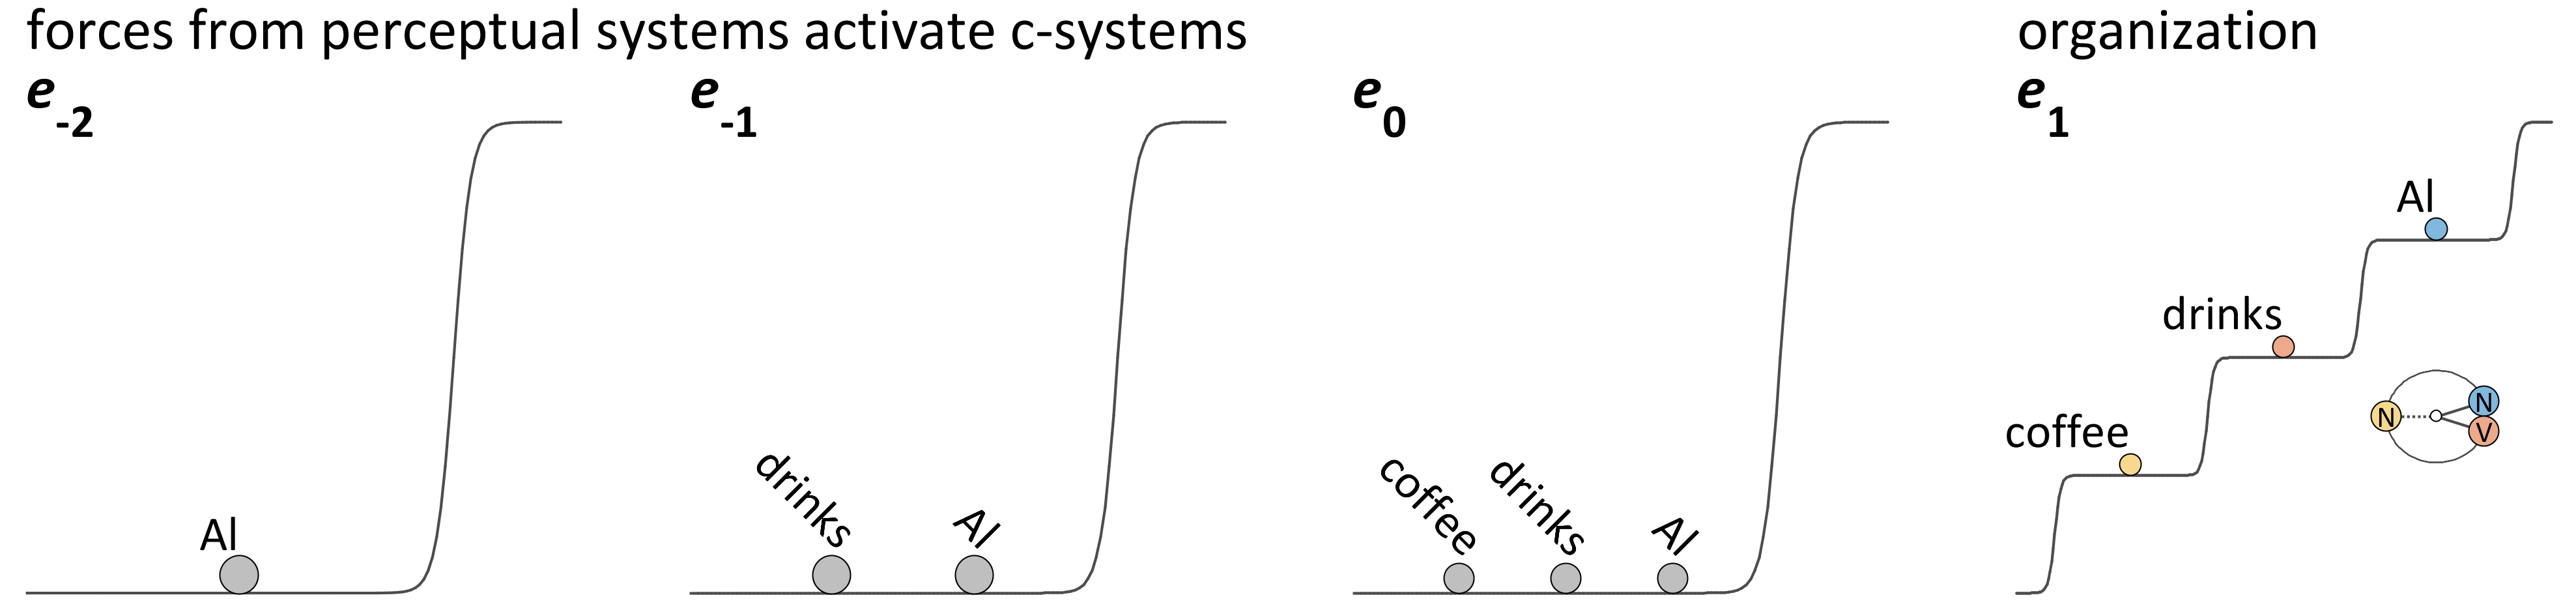
\includegraphics[width=\textwidth]{figures/Tilsen-img127.png}
\caption{Conceptual-syntactic systems are activated by perceptual systems.}
\label{fig:6:8}
\end{figure}

 

  To expand the empirical scope of our model of interpretation, incremental ϕ/e organization is necessary. However, the evolution of states during periods in which sensory systems activate cs-sys\-tems is generally unconstrained. {\figref{fig:6:9}} contrasts two highly ordered, memory stack-like trajectories in which systems are incrementally e-organized. In the precedency mapping, each newly activated system becomes excited and occupies the first above-ground level, while previously excited systems are each promoted one level. If the \isi{interpreter} enters a \isi{production regime}, the interpretation-production mechanism behaves as a first-in first-out buffer, in a sense. 

  
\begin{figure}
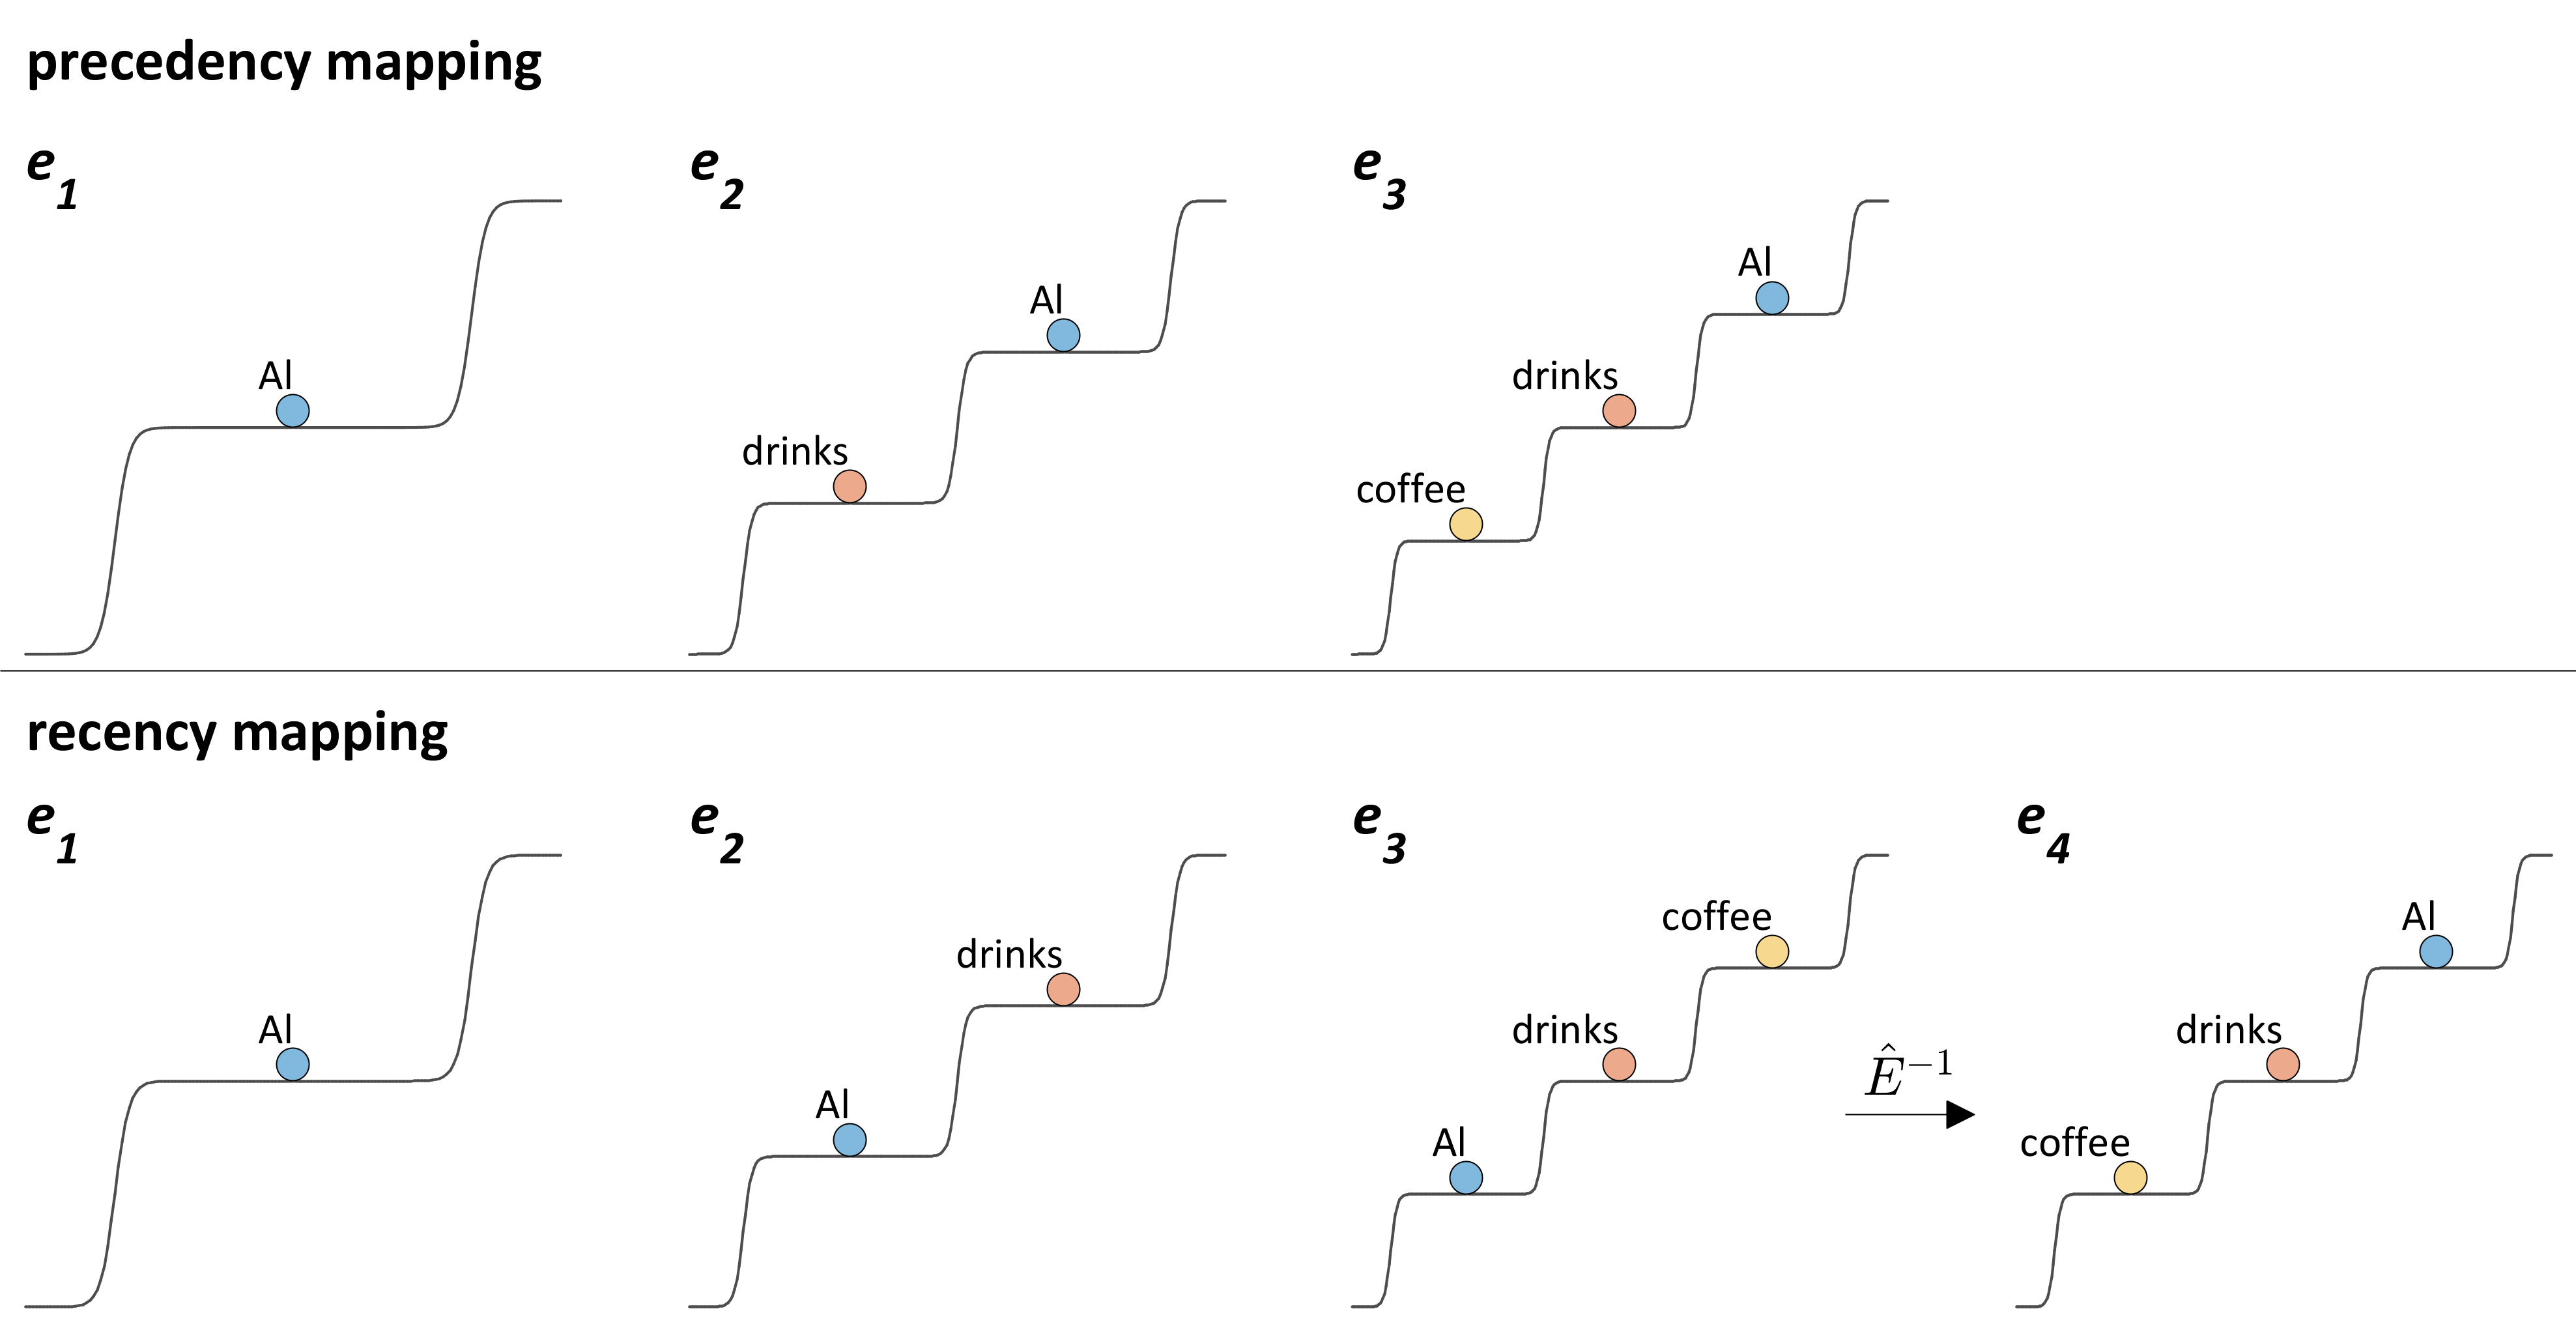
\includegraphics[width=\textwidth]{figures/Tilsen-img128.png}
\caption{Comparison of recency and precedency mappings in the e-or\-ga\-ni\-za\-tion of perceptually activated systems.}
\label{fig:6:9}
\end{figure}
 

  In the recency mapping, each newly excited system becomes the most highly excited system. In this case the relative excitations must be inverted before a production of the utterance could occur. This would suggest a new type of \isi{reorganization operator}, Ê\textsuperscript{{}inv}. This inversion operation is somewhat problematic because it does not seem to occur in other circumstances; it is an ad hoc set of operations that is necessary to convert the recency-based organization to one which is consistent with production.

  In any case, both precedency and recency incremental e-or\-ga\-ni\-za\-tion are probably too inflexible to be of much general use. Recall our depiction of the chaotic emergence of stable ϕ/e-con\-fi\-gu\-ra\-tions in production. We might expect something quite similar in interpretation: asymmetries in when individual sensory systems become active and exert forces on c- and s-sys\-tems, ambiguities in mappings from sensory systems to c- and s-sys\-tems, variation in the growth and competition timecourses of cs-resonances, inhomogeneity in the initial conditions, fluctuations in the \isi{surroundings} -- all of these make highly systematic organization scenarios such as those above quite unlikely.

  A somewhat more realistic picture is one in which ϕ-con\-fi\-gu\-ra\-tions arise incrementally and exert a strong influence on subsequent e-or\-ga\-ni\-za\-tion. Meaning relations can form as cs-sys\-tems become active, and part of the stabilization process involves excitation of those systems. Hence we expect ϕ-con\-fi\-gu\-ra\-tion emergence to bias e-or\-ga\-ni\-za\-tion. For example, in the \isi{interpretation trajectory} of \textit{Bo knows Al drinks coffee} below, ϕ-con\-fi\-gu\-ra\-tions are organized as soon as the relevant cs-sys\-tems are active. In the subsequent examples, we show the most recently perceived system as grounded in the epoch prior to the one in which it becomes excited.  Hence [knows]\{V\} is active in the epoch (e2), prior to participating in the configuration {\textbar}Bo knows{\textbar} in (e3). Likewise, [Al]\{N\} is active in (e3) and through a \isi{selective reorganization} becomes excited in (e4). Incrementally organized states bias subsequent reorganizations. For example, the incrementally organized {\textbar}Al drinks{\textbar} state in epoch (e5) biases the system to reorganize to (e6), where {\textbar}Al drinks coffee{\textbar} is excited. 

  
\begin{figure}
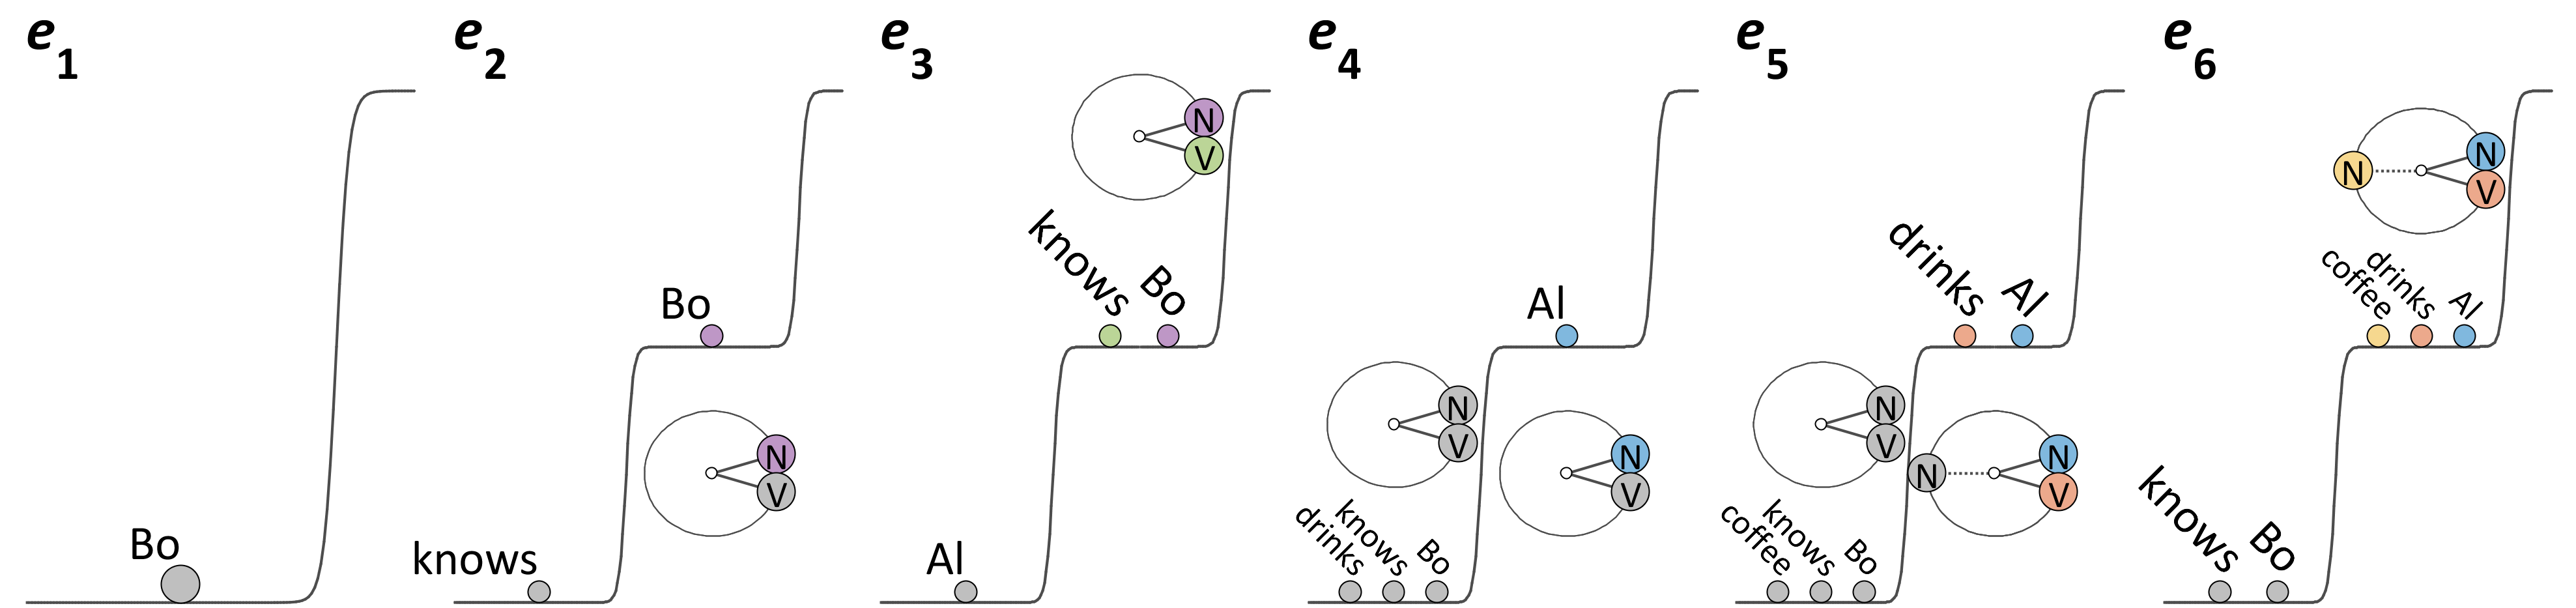
\includegraphics[width=\textwidth]{figures/Tilsen-img129.png}
\caption{The immediate organization bias in incremental ϕ organization.}
\label{fig:6:10}
\end{figure}
 

  The excitation of [Bo][knows] in (e3) is hypothesized to result from an expectation that a newly active cs-sys\-tem will enter into a ϕ-con\-fi\-gu\-ra\-tion with previously excited systems, without any intervening ϕ-con\-fi\-gu\-ra\-tions being organized. In our framework an “expectation” of this sort can be conceptualized as forces which promote coupling of a newly activated cs-sys\-tem with an already activated or excited system. We refer to this as the \textit{\isi{immediate organization} bias}, and consider it to be the basis for \isi{incremental organization}. Immediate organization explains why utterances such as \textit{Al, Bo knows, drinks coffee} are more difficult to parse: the \isi{interpreter} cannot couple [Bo]\{N\} with the previously activated/excited system, [Al]\{N\}.

  One empirically desirable consequence of \isi{incremental organization} and the \isi{immediate organization bias} is that a ϕ-con\-fi\-gu\-ra\-tion can prevent a newly excited system from participating in a stable configuration. To see why, consider the utterance in \REF{ex:6:12}: 

\ea\label{ex:6:12}
Al drinks coffee and tea is brewing.
\z   

  This sentence is designed to create a \isi{garden path} effect. The \isi{interpreter} may initially understand \textit{tea} as an object of \textit{drinks}, because of the \isi{immediate organization bias}. A possible \isi{interpretation trajectory} is shown in {\figref{fig:6:11}}. (Note that the trajectory here and in examples to follow depict incremental e-or\-ga\-ni\-za\-tion, but this is not strictly necessary. The e-or\-ga\-ni\-za\-tion serves only to facilitate the depiction of the relevant ϕ-con\-fi\-gu\-ra\-tions). The \isi{garden path} \isi{relational meaning} experience of \textit{drinks tea} corresponds to [tea]\{−N\} and [drinks]\{V\} being in a ϕ-con\-fi\-gu\-ra\-tion, shown in epoch (e3).  However, [brew]\{V\} must −ϕ couple to a \{−N\} system in order to be coherent. Grounding of the {\textbar}drinks tea{\textbar} configuration prevents [brew]\{V\} and [tea]\{−N\} from being in a stable configuration. The inability of [tea]\{−N\} to couple to both [drinks]\{V\} and [brew]\{V\} is due to the \isi{selective reorganization} from (e4) to (e5). The \isi{interpreter} may then become aware of the non-\isi{coherence} of the state in (e5). This awareness induces a grounding of all systems (e6) and reorganization to the state in (e7). 

  
\begin{figure}
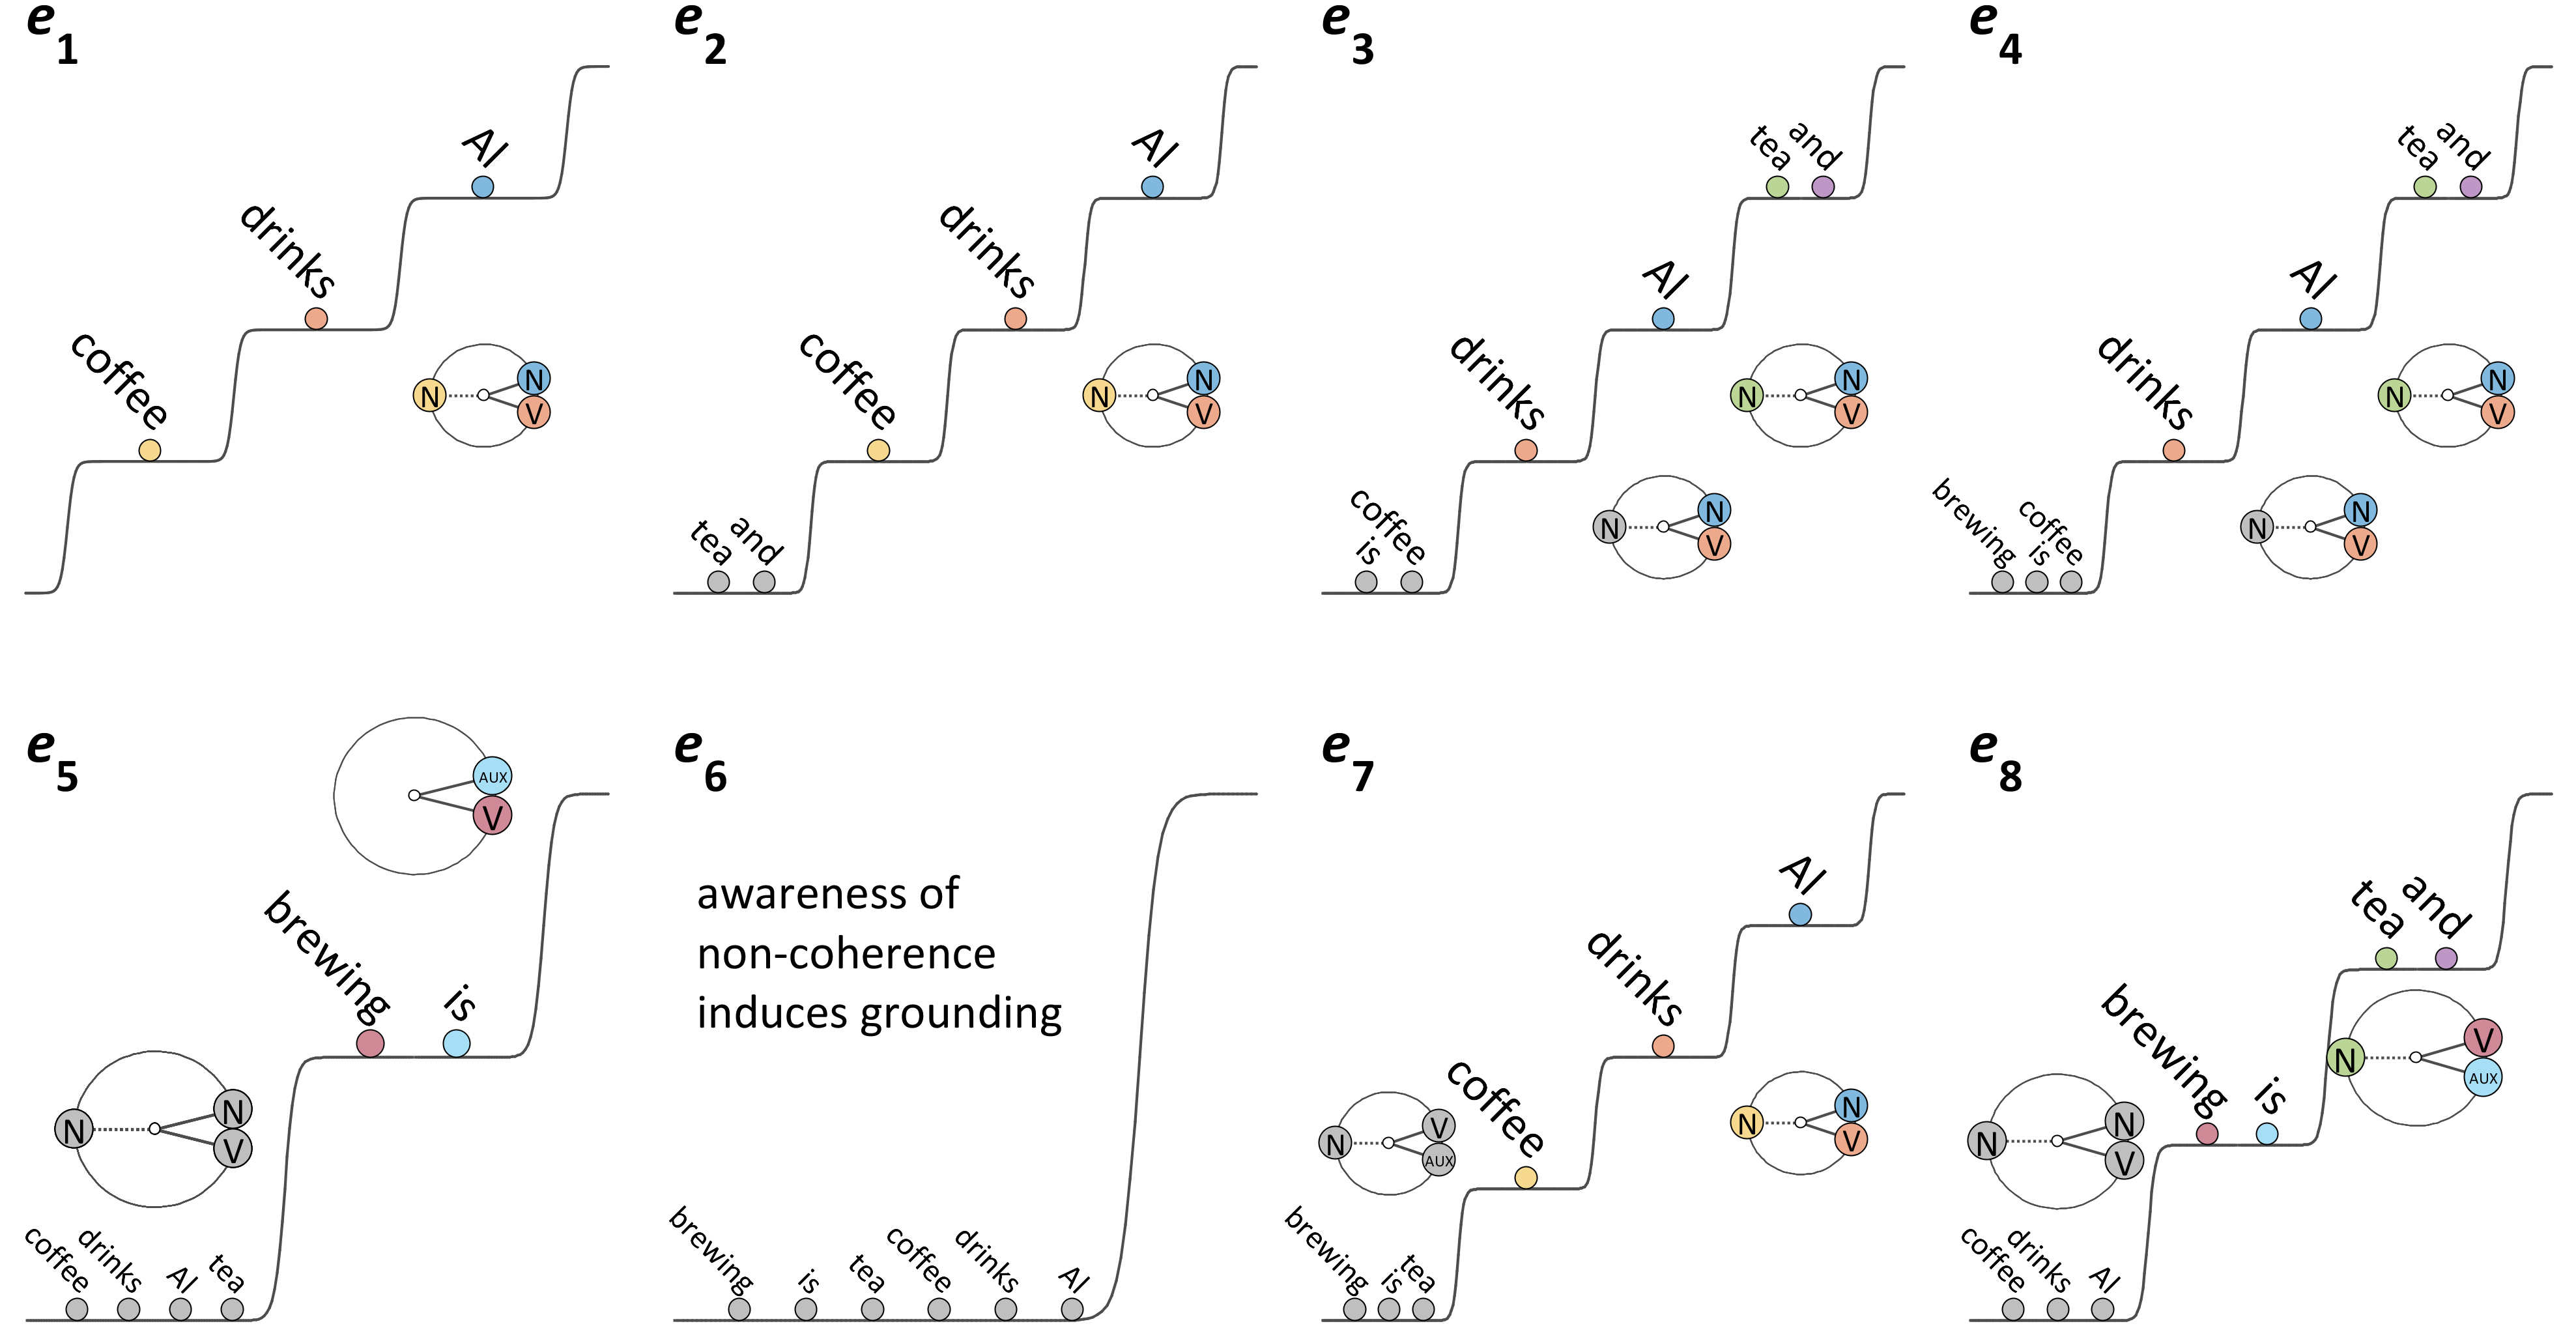
\includegraphics[width=\textwidth]{figures/Tilsen-img130.png}
\caption{A garden path trajectory in which awareness of non-coherence induces grounding and reorganization.}
\label{fig:6:11}
\end{figure}
 

  On the other hand, the above utterance might not induce a \isi{garden path} effect. The \isi{garden path} arises because the \isi{selective reorganization} Ê\textsubscript{2} grounds only [coffee]\{N\}, as in {\figref{fig:6:12}}(A). Alternatively, if the \isi{selective reorganization} Ê\textsubscript{2} occurs as in (B), grounding {\textbar}Al drinks coffee{\textbar}, then [tea]\{N\} does not couple with [drinks]\{V\} and can couple with [brew]\{V\} in (e3).

  
\begin{figure}
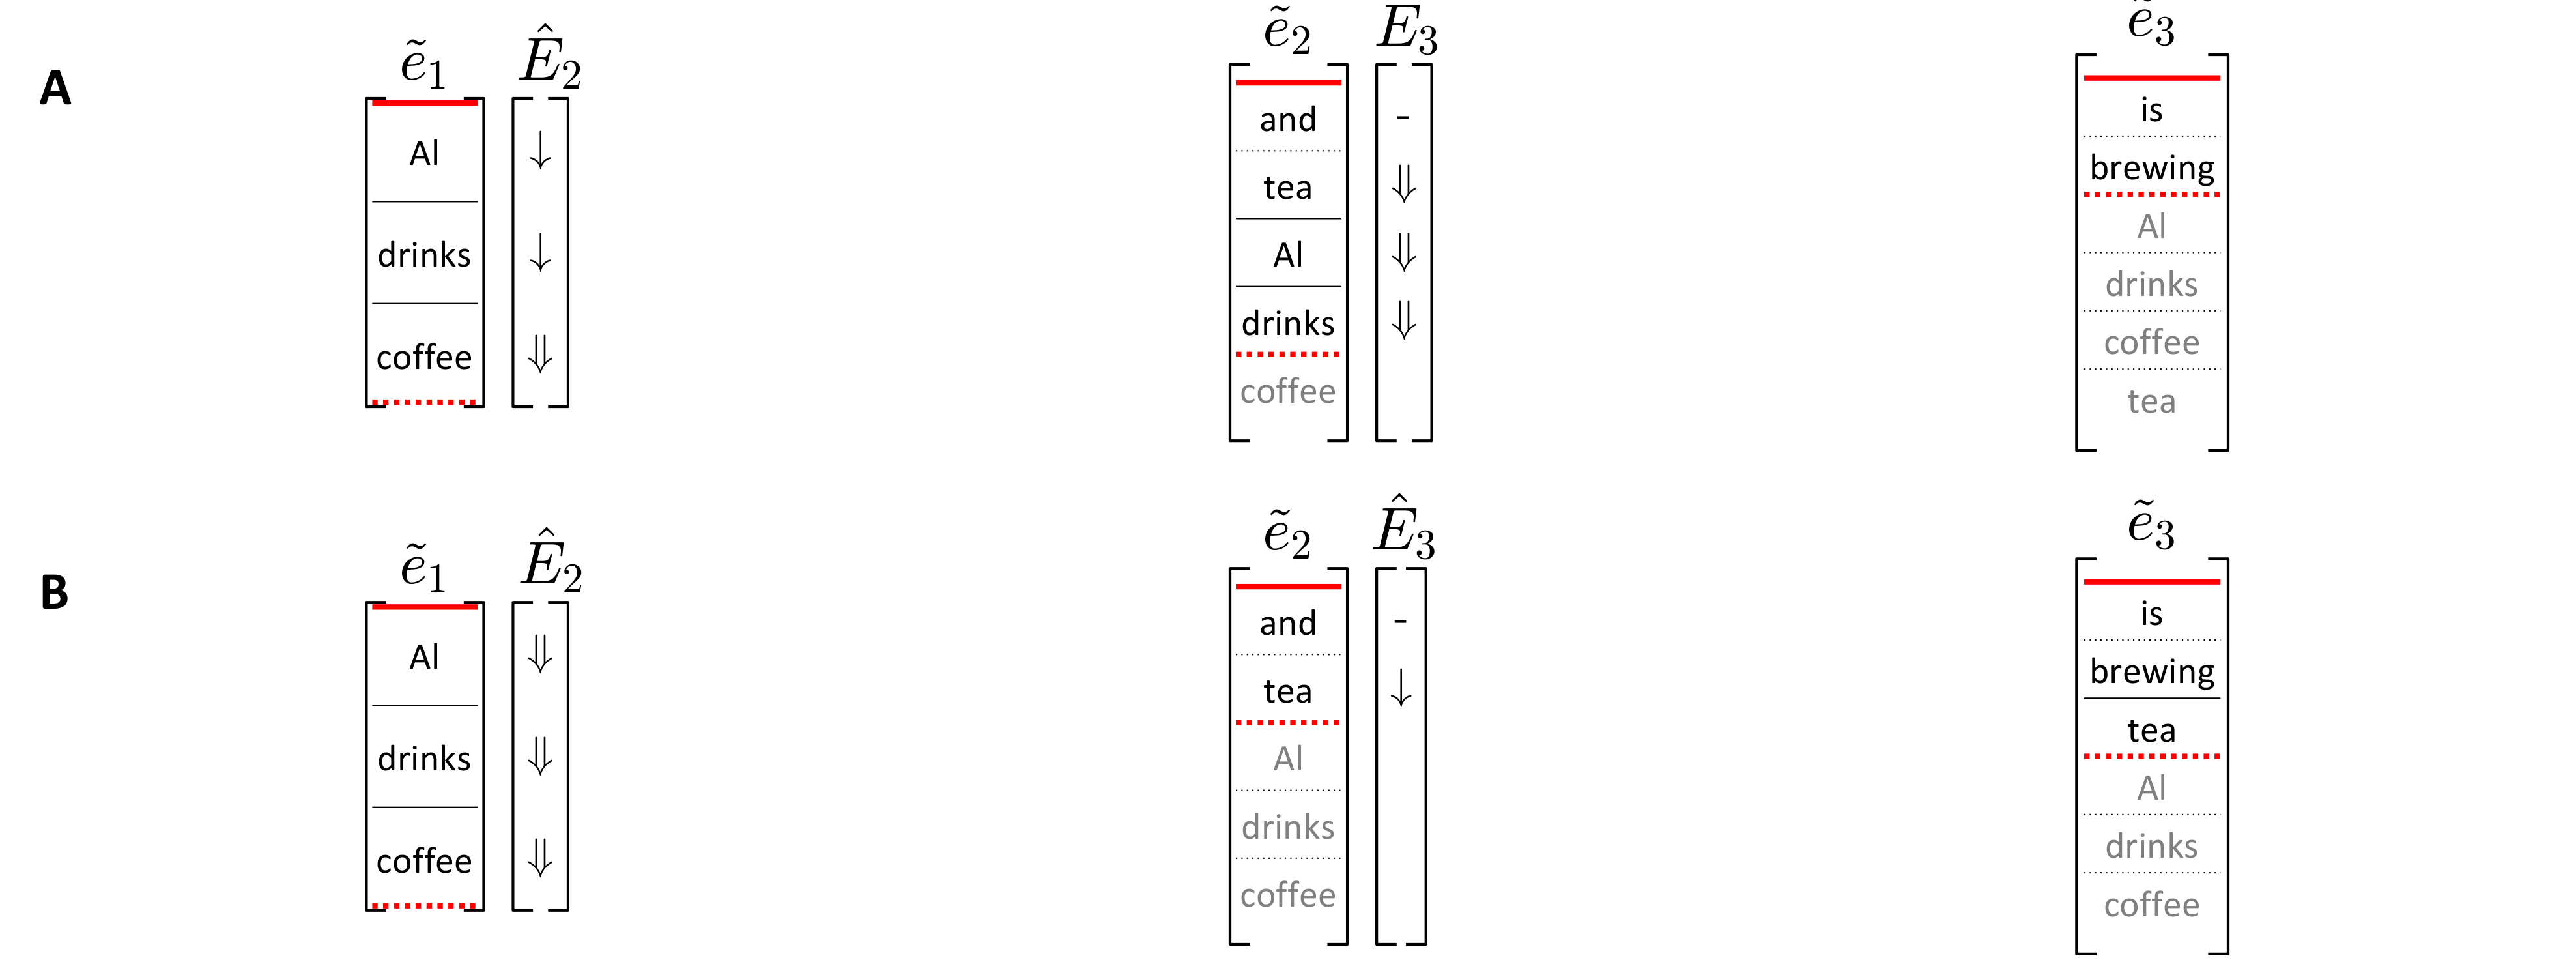
\includegraphics[width=\textwidth]{figures/Tilsen-img131.png}
\caption{A garden path occurs with the selective reorganization in (A) but not with the selective reorganization in (B).}
\label{fig:6:12}
\end{figure}
 

  The \isi{selective reorganization} in (B) which grounds all of the cs-sys\-tems associated with {\textbar}Al drinks coffee{\textbar} would be more likely to occur in interpretation when the utterance is spoken slowly (or when a comma is present: \textit{Al drinks coffee, and tea is brewing}), and less likely to occur when it is spoken quickly. Thus we can view \isi{prosodic} manipulations such as boundary-lengthening as a mechanism for diminishing the forces which give rise to the \isi{immediate organization bias}.

  Our analysis of the \isi{garden path} repair raises the question of how the \isi{interpreter}, after becoming aware of the incoherence of the configuration in (e5), knows to reorganize so that [tea]\{N\} and [brew]\{V\} are coupled. This is an important, challenging question, which deserves future attention. In some circumstances, the \isi{interpreter} does not -- without assistance -- achieve a coherent reorganization. This suggests that the {\textbar}drink tea{\textbar} system may not be sufficiently decoupled by grounding. The assistance, in everyday conversation, may be in the form of \isi{intonation} (\textit{Al drinks coffee, … and tea is brewing}). Indeed, even in the textbook example (\textit{the horse raced past the barn fell}), some students who are unfamiliar with the example must be explicitly cued to evoke the relevant configuration (i.e. with \textit{the horse that was raced…}) before they are able to achieve a \isi{coherent interpretation}. 

  Garden path phenomena are a subset of a more general circumstance in which the system trajectory gets trapped in some subspace, preventing the trajectory from evolving to other possible states. In the prototypical \isi{garden path}, the utterance is non-coherent when the system trajectory enters the trapping region, but more generally, the trapping subspace may be coherent and simply prevents some alternative, potentially coherent trajectory from occurring. This is why ambiguities can be difficult to notice. Consider the sentence in \REF{ex:6:13}:

  \ea\label{ex:6:13}
    {Al drinks soda coffee and tea are my favorites.}
   \z
   
  In interpretation of \REF{ex:6:13}, \isi{immediate organization} creates a strong bias for a {\textbar}Al drinks soda{\textbar} configuration to arise. This prevents the alternative \isi{coherent interpretation} in which the producer means that \textit{Al}, \textit{drinks}, \textit{soda}, \textit{coffee}, and \textit{tea} are their favorite things. The trapping substate here is a cs-resonance of [drinks] with \{V\}, which prevents a [drinks]\{N\} system from being excited. There are many circumstances in which \isi{garden path} effects can arise (\citealt{FFerreira2005,Pritchett1988}), and comparisons of behavior in these should provide valuable information regarding \isi{incremental organization}. 

  It should be noted here that the o/el conception does not gel with certain types of probabilistic models in which representations themselves are considered probabilistic (e.g. \citealt{ChaterManning2006,Manning2003}). The system state is unarguably deterministic: there is one and only one state at any given moment of time, and so we should not reason that there are multiple parses of an utterance, each associated with a probability. Certainly, multiple configurations may be simultaneously active, to varying degrees, but this differs conceptually and implementationally from models in which a unity normalization is applied to construct a probability distribution over states.

  Incremental e-or\-ga\-ni\-za\-tion is also relevant to understanding why “word salad” utterances such as those in \REF{ex:6:14} do not typically lead to \isi{coherence}. In the marginal cases, \isi{intonation}/punctuation can facilitate \isi{coherence} when (in fixed order languages) the e-or\-ga\-ni\-za\-tion deviates from the typical ϕ-e mapping. We infer from these examples that \isi{incremental organization} is influenced by learned ϕ-to-e mappings. What is important about this, from the perspective of our conceptual model, is that interpretation does not necessarily have access to ϕ relations. Interpreters may need to use e-to-ϕ mappings, which are inversions of learned ϕ-to-e mappings, in conjunction with \isi{immediate organization}. Intonation/punctuation may diminish the influence of \isi{immediate organization} on \isi{incremental organization}. 

\ea\label{ex:6:14}
  \ea[*]{Al coffee knows drinks Bo.}  
  \ex[*]{Bo drinks Al knows coffee.}
  \ex[*]{Coffee Bo Al drinks knows.}
  \ex[?]{Al Bo knows drinks coffee.\hspace{0.5cm}cf. Al -- Bo knows -- drinks coffee.}
  \ex[?]{Coffee Bo knows Al drinks.\hspace{0.5cm}cf. Coffee -- Bo knows -- Al drinks.}
  \ex[?]{Bo Al drinks coffee knows.\hspace{0.5cm}cf. \textsuperscript{?}Bo -- Al drinks coffee -- knows.}
\z
\z

In \REF{ex:6:14}(a--c), there seems to be no amount of \isi{intonational}/punctuational information which can make the highly abnormal mappings coherent. This suggests that, because of the \isi{immediate organization bias}, substantial departures from learned ϕ-e mappings make achieving \isi{coherence} more difficult. What constitutes a “substantial” departure is an open question.

\subsection{Factors which influence coherence experiences}

It is important to view \isi{grammatical coherence} as a phenomenon which is associated with an \textit{experience}. More specifically, we experience a trajectory of \isi{relational meaning} configurations which may or may not be stable. Although our generic hypothesis is that \isi{grammaticality}/\isi{acceptability} intuitions reflect these experiences, we have not considered which aspects of the trajectory our intuitions are sensitive to. A comprehensive study of intuitions should consider a wide variety of factors, e.g. the number of simultaneously excited ϕ-con\-fi\-gu\-ra\-tions, ϕ-con\-fi\-gu\-ra\-tions in which some systems are active but unexcited, activation of systems which cannot be immediately organized, \isi{interference} from \isi{s-sys\-tem differentiation}, \isi{interference} from c-sys\-tem differentiation, the ϕ of differentiated systems, previously active systems which interfere with the excitation of newly active cs-sys\-tems from being organized, etc. 

  Here we focus on \isi{interference}, which seems to underlie many of the factors listed above in some way or another. The \isi{immediate organization bias} can also be seen as a mechanism which minimizes \isi{interference} by stabilizing newly activated systems as soon as possible. Consider the sentences in \REF{ex:6:15}-\REF{ex:6:18}, where in each set of sentences, the (a) examples seem more acceptable than the (b) examples, which are in turn more acceptable than the (c) examples. Furthermore, center embedding sentences in \REF{ex:6:15} and \REF{ex:6:16} are generally less coherent than their \isi{tail recursion} counterparts in \REF{ex:6:17} and \REF{ex:6:18}.  

\ea\label{ex:6:15}
\textbf{Center embedding}\\
    \ea I saw a frog a cat chased.                      
    \ex I saw a frog a cat a dog bit, chased.  
    \ex I saw a frog a cat a dog a bee stung bit chased.
    \z
\z

\ea\label{ex:6:16}
\textbf{Center embedding}\\
    \ea\label{ex:6:16a} I saw Al, who Bo likes.                                
    \ex\label{ex:6:16b} I saw Al, who Bo, who Cam likes, likes.                
    \ex\label{ex:6:16c} I saw Al, who Bo, who Cam, who Dee likes, likes, likes.
    \z
\z

\ea\label{ex:6:17}
\textbf{Tail recursion}\\
    \ea I saw a cat who chased a frog.
    \ex I saw a dog who bit a cat, who chased a frog.
    \ex I saw a bee who stung a dog who bit a cat who chased a frog.
    \z
\z

\ea\label{ex:6:18}
\textbf{Tail recursion}\\
    \ea I saw Bo, who likes Al.
    \ex\label{ex:6:18b} I saw Cam, who likes Bo, who likes Al.
    \ex\label{ex:6:18c} I saw Dee, who likes Cam, who likes Bo, who likes Al.
    \z
\z
  

  A hypothesized \isi{interpretation trajectory} for the center embedding of relative clauses in \REF{ex:6:16b} is shown in {\figref{fig:6:13}}. Note that we have omitted some intervening epochs in the trajectory to avoid clutter. As we hypothesized earlier the object relative [who]\{\textsc{rel}\} system +ϕ couples to the relativized \{N\} and −ϕ couples to a \{V\}. Thus in (e2) a [who]\{\textsc{rel}\} system +ϕ couples to [Al]\{N\}, and in (e3) a [who]\{\textsc{rel}\} system +ϕ couples to [Bo]\{N\}. We conceptualize these [who]\{\textsc{rel}\} systems as differentiations of a general \{\textsc{rel}\} system, just like [Al]\{N\} and [Bo]\{N\} are differentiations of \{N\}. Furthermore, we assume that a system is grounded after having participated in its expected ϕ-con\-fi\-gu\-ra\-tion, unless that system is relativized. Hence we imagine that [I]\{\textsc{PRO}\} and [saw]\{V\} are grounded after (e1) but [Al]\{N\} remains above-ground because it couples with [who]\{\textsc{rel}\} in (e2). Thus \{\textsc{rel}\} systems cause some other system to which they are coupled to remain excited.

  
\begin{figure}
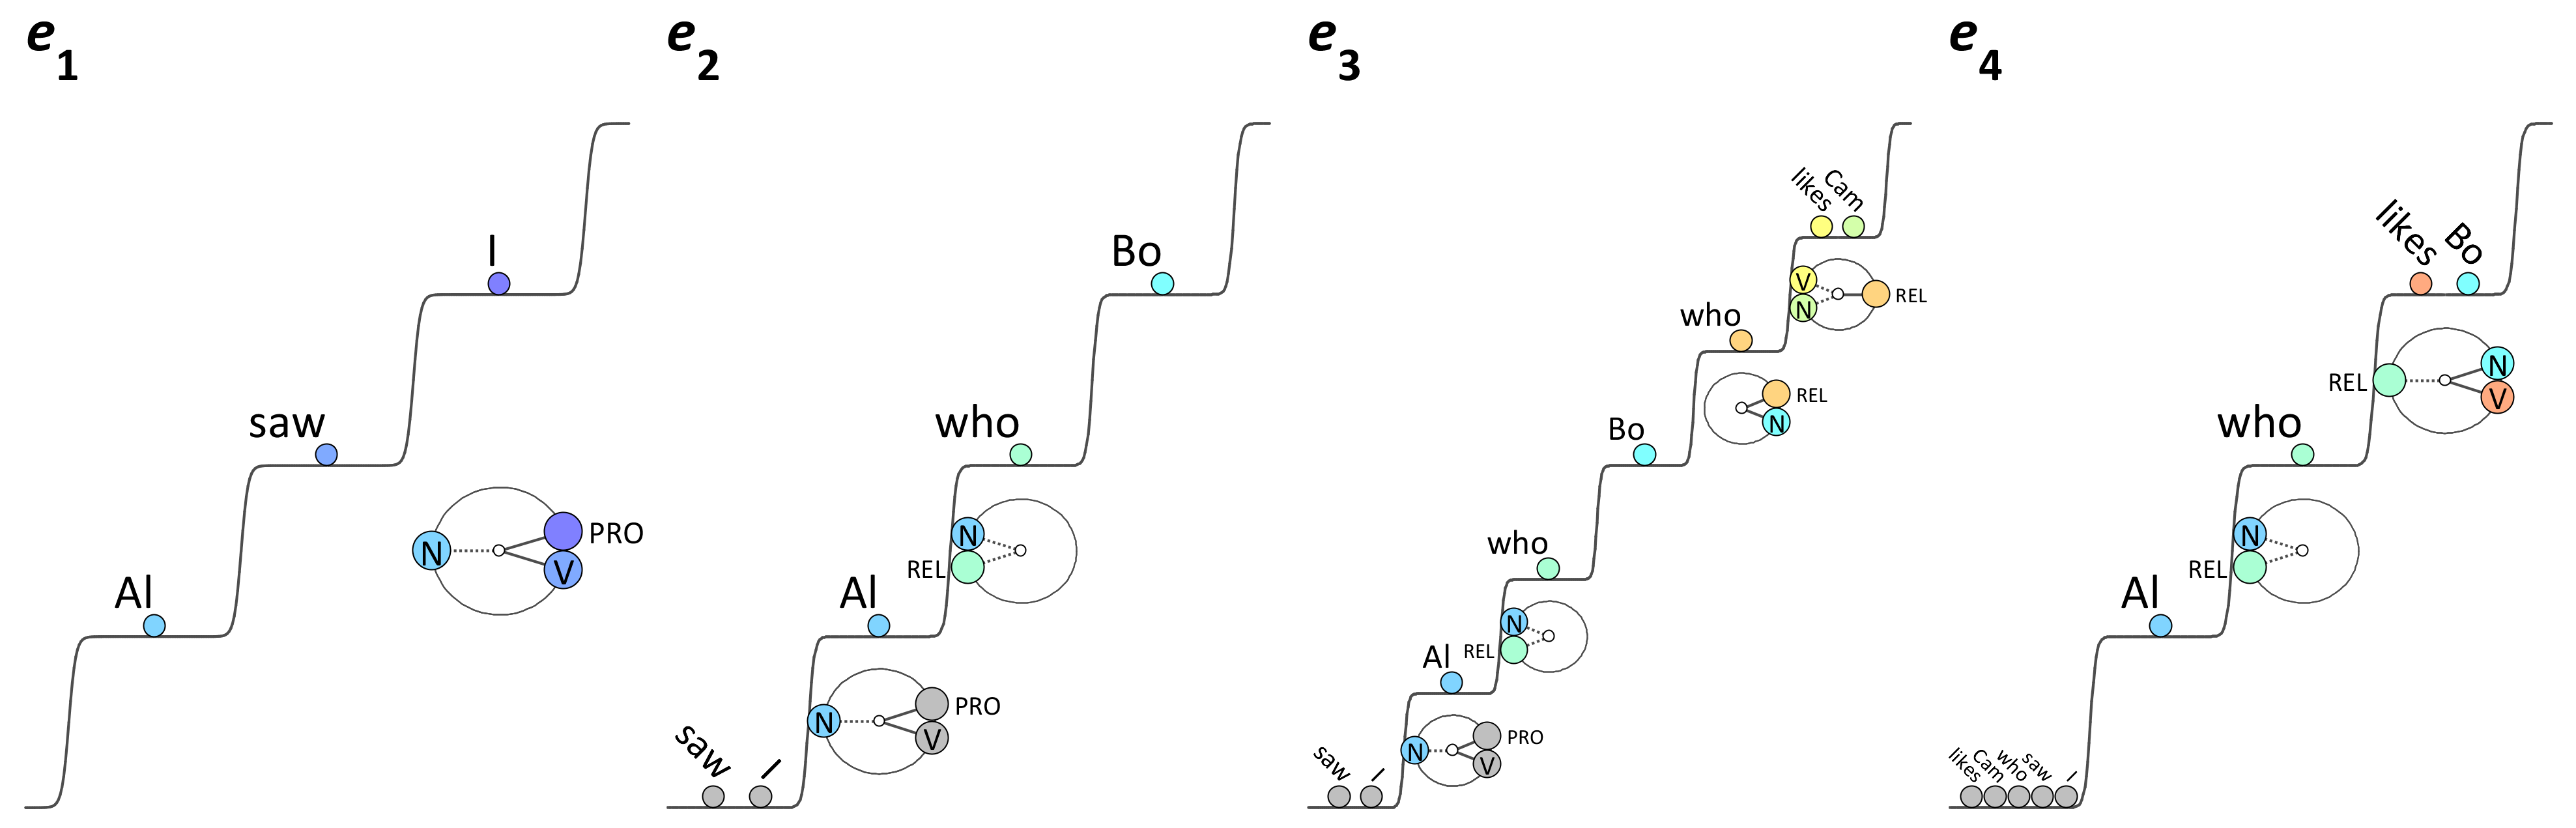
\includegraphics[width=\textwidth]{figures/Tilsen-img132.png}
\caption{Interpretation trajectory for a center-embedded relative clause.}
\label{fig:6:13}
\end{figure}
 

  Given the above analysis, the first question we ask is: why is \REF{ex:6:16b} less likely to induce a coherent state than \REF{ex:6:16a}? One simple difference is that \REF{ex:6:16b} requires more ϕ-con\-fi\-gu\-ra\-tions to be simultaneously excited than \REF{ex:6:16a}. This follows from our hypothesis that each [who]\{\textsc{rel}\} system +ϕ couples to an \{N\} and −ϕ couples to a \{V\}, along with our assumption that systems coupled to \{\textsc{rel}\} remain excited to participate in a configuration in a subsequent epoch. Having multiple systems of the same class simultaneously excited is potentially problematic because of differentiation \isi{interference}. In the example there is s-differentiation \isi{interference} between [Al]\{N\}, [Bo]\{N\}, and [Cam]\{N\}, and between [saw]\{V\} and [likes]\{V\}. There is also c-differentiation \isi{interference} between [who] systems, and between [likes] systems, although the [likes] subsystems are not simultaneously excited. 

  Interestingly, because of the ϕ-con\-fi\-gu\-ra\-tion invariance principle, [Al]\{N\} and [Bo]\{N\} must have a ϕ-distal relation, while [Al]\{N\} and [Cam]\{N\} must have a ϕ-proximal relation. This follows from our hypotheses regarding role-to-ϕ patterns for [who]\{\textsc{rel}\}, \isi{transitive} \{V\}, and agent/patient role \{N\}. Note that we use the term \textit{relation} here rather than configuration because we do not want to imply that the ϕ pattern arises directly from ϕ-coupled s-sys\-tems. The [Al], [Bo], and [Cam] \{N\} systems must interfere through s-differentiation. Because \REF{ex:6:16b} is substantially worse than \REF{ex:6:16a}, we might guess that the differentiation associated with proximally ϕ-related [Al]\{N\} and [Cam]\{N\} induces more \isi{interference} than the differentiation associated with the distally ϕ-related [Al]\{N\} and [Bo]\{N\}. This makes a lot of sense given our speculation that \{N\} to \{+N\}/\{−N\} differentiation is relatively unproblematic compared to differentiation within \{+N\} or \{−N\}. In other words, differentiation of a system into two systems with proximal ϕ may induce more \isi{interference} than differentiation into two systems with distal ϕ.

  Perhaps most problematically, there is an epoch of the center embedding interpretation in which a newly activated system cannot be immediately organized. Specifically, in (e2) [Bo]\{N\} is coupled with a \{\textsc{rel}\} system but is not coupled to any lexical \{V\} system in (e3). 

  Indeed, the reason that the tail-recursive utterances in \REF{ex:6:17} and \REF{ex:6:18} are more coherent than their center-embedded counterparts in \REF{ex:6:15} and \REF{ex:6:16} is that each newly activated system can be immediately organized. A possible \isi{interpretation trajectory} for the tail-\isi{recursion} of \REF{ex:6:18c} is shown in {\figref{fig:6:14}}. 

  
\begin{figure}
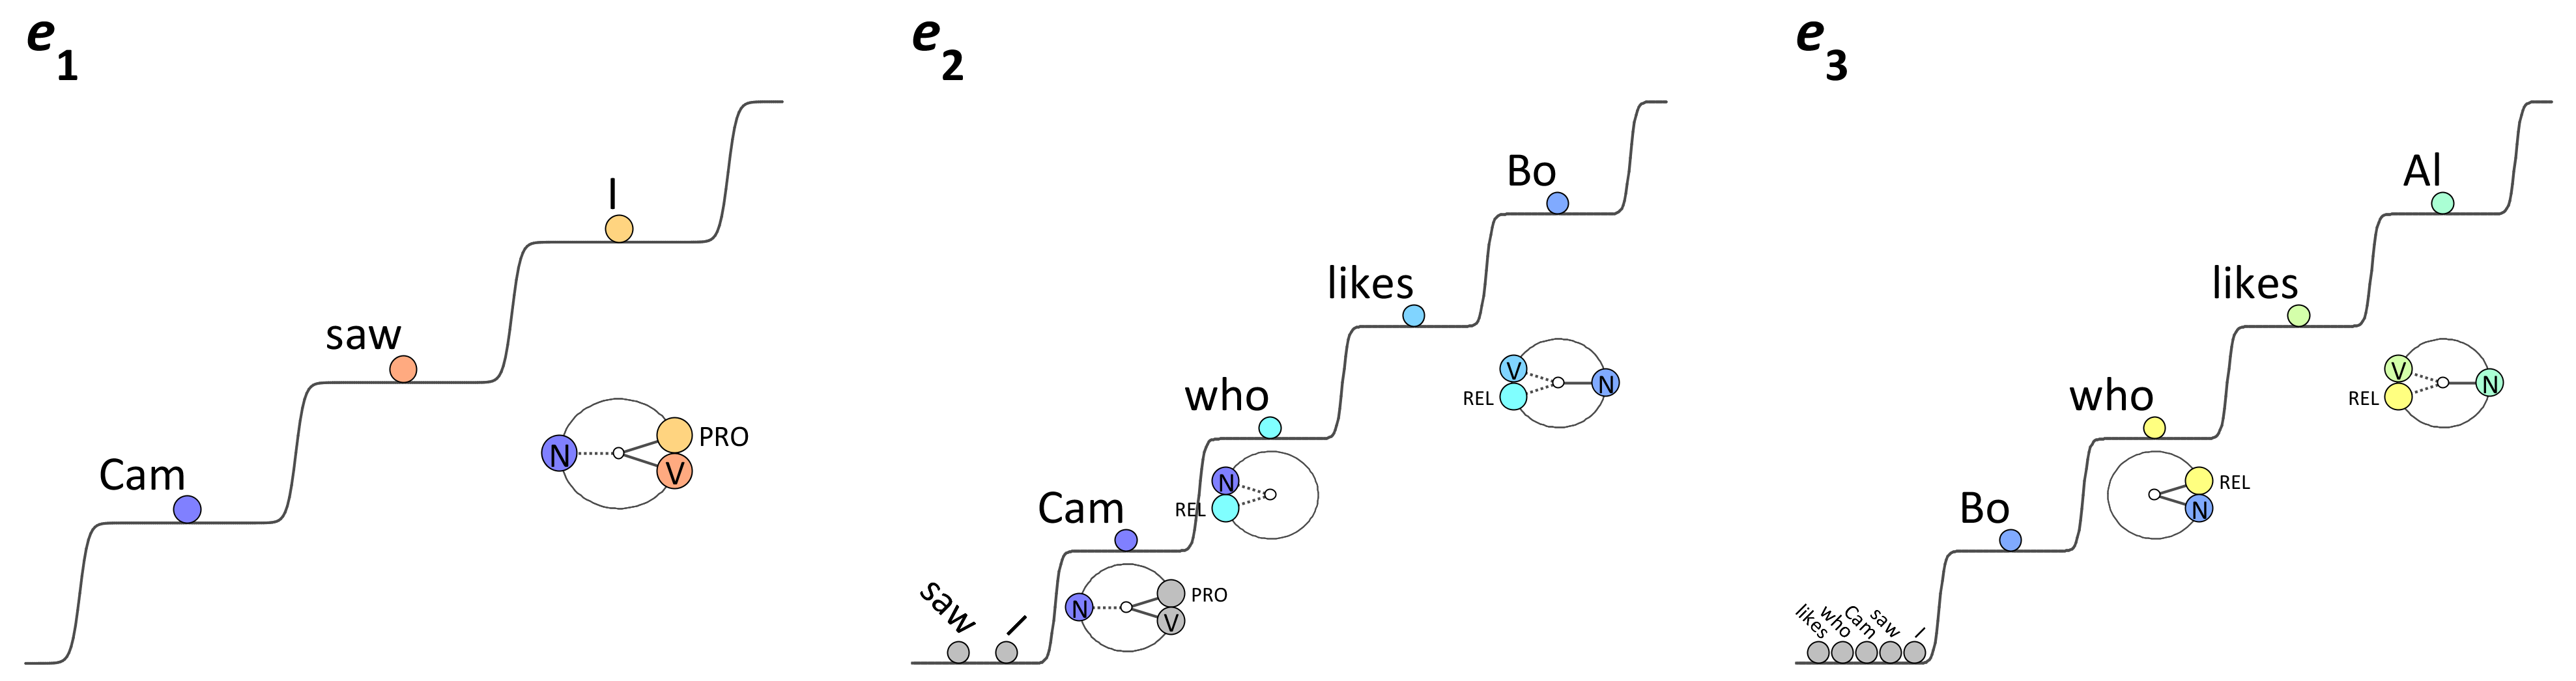
\includegraphics[width=\textwidth]{figures/Tilsen-img133.png}
\caption{Tail-recursive trajectory: newly activated systems can be immediately organized.}
\label{fig:6:14}
\end{figure}
 

  The tail-\isi{recursion} in {\figref{fig:6:14}} does not have any epochs in which a newly activated cs-sys\-tem does not ϕ-couple to any previously activated or excited \isi{lexical system}. In (e2) [Bo]\{N\} couples with [likes]\{V\} before the \{\textsc{rel}\} system couples to [Bo]\{N\}. This contrasts with (e2) of the center embedding in {\figref{fig:6:13}}, where [Bo]\{N\} couples with \{\textsc{rel}\}, and where epochs in which the {\textbar}Cam likes{\textbar} configuration arises intervene before the {\textbar}Bo likes{\textbar} configuration is organized. Furthermore, the {\textbar}likes who{\textbar} configuration in (e2) of the \isi{tail recursion} trajectory can be grounded in the transition to (e3), which avoids the circumstance where two \{N\}\{\textsc{rel}\} configurations are excited. Loosely speaking, we can attribute the difference in \isi{grammaticality} intuitions for center embedding and \isi{tail recursion} to difficulty in “keeping things in memory” longer. But more usefully, we see that the difficulty is the instability of keeping an \{N\} excited when it is not ϕ-coupled with a \{V\} and interferes with other \{N\} systems. In other words, coupling to \{V\} helps stabilize \{N\} systems and thereby diminishes \isi{interference} between simultaneously excited \{N\} systems.

  In addition to \isi{interference}, “contextual” factors, i.e. the state of the \isi{surroundings} prior to an interpretation, must have an influence on \isi{coherence}. Consider the utterance in \REF{ex:6:19}:

  \ea\label{ex:6:19}
    {read you a book on modern music?}
\z

The utterance in \REF{ex:6:19} probably does not induce a coherent trajectory on first interpretation. Now, read the list of utterances in \REF{ex:6:20}:

\ea\label{ex:6:20}
\ea {have you a book on modern music?}
\ex {have you a book on ancient music?}
\ex {have you a dictionary of English?}
\ex {want you a dictionary of English?}
\ex {want you a book on ancient music?}
\ex {want you a book on modern music?}
\ex {seen you a book on modern music?}
\ex {seen you a book on ancient music?}
\ex {seen you a dictionary of English?}
\ex {read you a dictionary of English?}
\ex {read you a book on ancient music?}
\ex {read you a book on modern music?}
\z
\z

  The repetition of similar trajectories induces a \isi{structural priming} effect. The last sentence coheres much more quickly than it did the first time around. Such effects suggest that every time some particular state trajectory occurs, trajectories which require a similar pattern of re-or\-ga\-ni\-za\-tions can occur more quickly or with less \isi{interference}, in interpretation of subsequent utterances. A variety of empirical studies provide evidence that such priming of this sort occurs and can have effects on a multi-day timescale (\citealt{BockEtAl2007,VSFerreiraEtAl2006,Nagata1988,Nagata1992,PickeringFerreira2008,RowlandEtAl2012}). We can view such learning as \isi{macroscale} changes in the forces which regulate ϕ-to-e mapping: the forces are altered to favor trajectories which are similar to a recently experienced one. There are many interesting questions that one might ask regarding the timescales on which such effects arise.

In contrast to the factors mentioned above, which are generally associated with \isi{interference}, \isi{grammatical coherence} does not appear to be as strongly affected by flavors of \isi{relational meaning}. This can be inferred from the classic \textit{colorless green ideas} example \citep{Chomsky1956}, which does not evoke a strong unacceptability intuition. It does, however, seem to induce an atypical \isi{meaning experience}.
 
\ea
colorless green ideas sleep furiously
\z 

  The example satisfies the \isi{utterance coherence} criteria, and there is no reason to posit any particularly strong \isi{interference}. Any oddness we experience in interpretation of the utterance must therefore derive from some other mechanism. One possible account of the oddness of the experience involves an aggregate effect of weakly activated, weakly interacting c-sys\-tems. Recall that we have assumed that interactions between c-sys\-tems are typically not very strong, particularly between lexical c-sys\-tems. This assumption is important because strong interactions would compromise flexibility of \isi{relational meaning} experiences. Yet weak interactions are not the same as no interactions. Indeed, whenever a c-sys\-tem is excited, many other c-sys\-tems must become active. Although we typically omit them from representations, these grounded systems may in the aggregate have a substantial effect on other c-sys\-tems. In {\figref{fig:6:15}} we imagine that excitation of [green] induces ground-level excitation of many other c-sys\-tems that are associated with [green] (such as [leaf], [grass], [emerald], [apple], etc.), which we label as <green>. The c-sys\-tems <green> which are primed by [green] interact weakly with all of the c-sys\-tems <colorless> which are primed by [colorless]. 

  
\begin{figure}
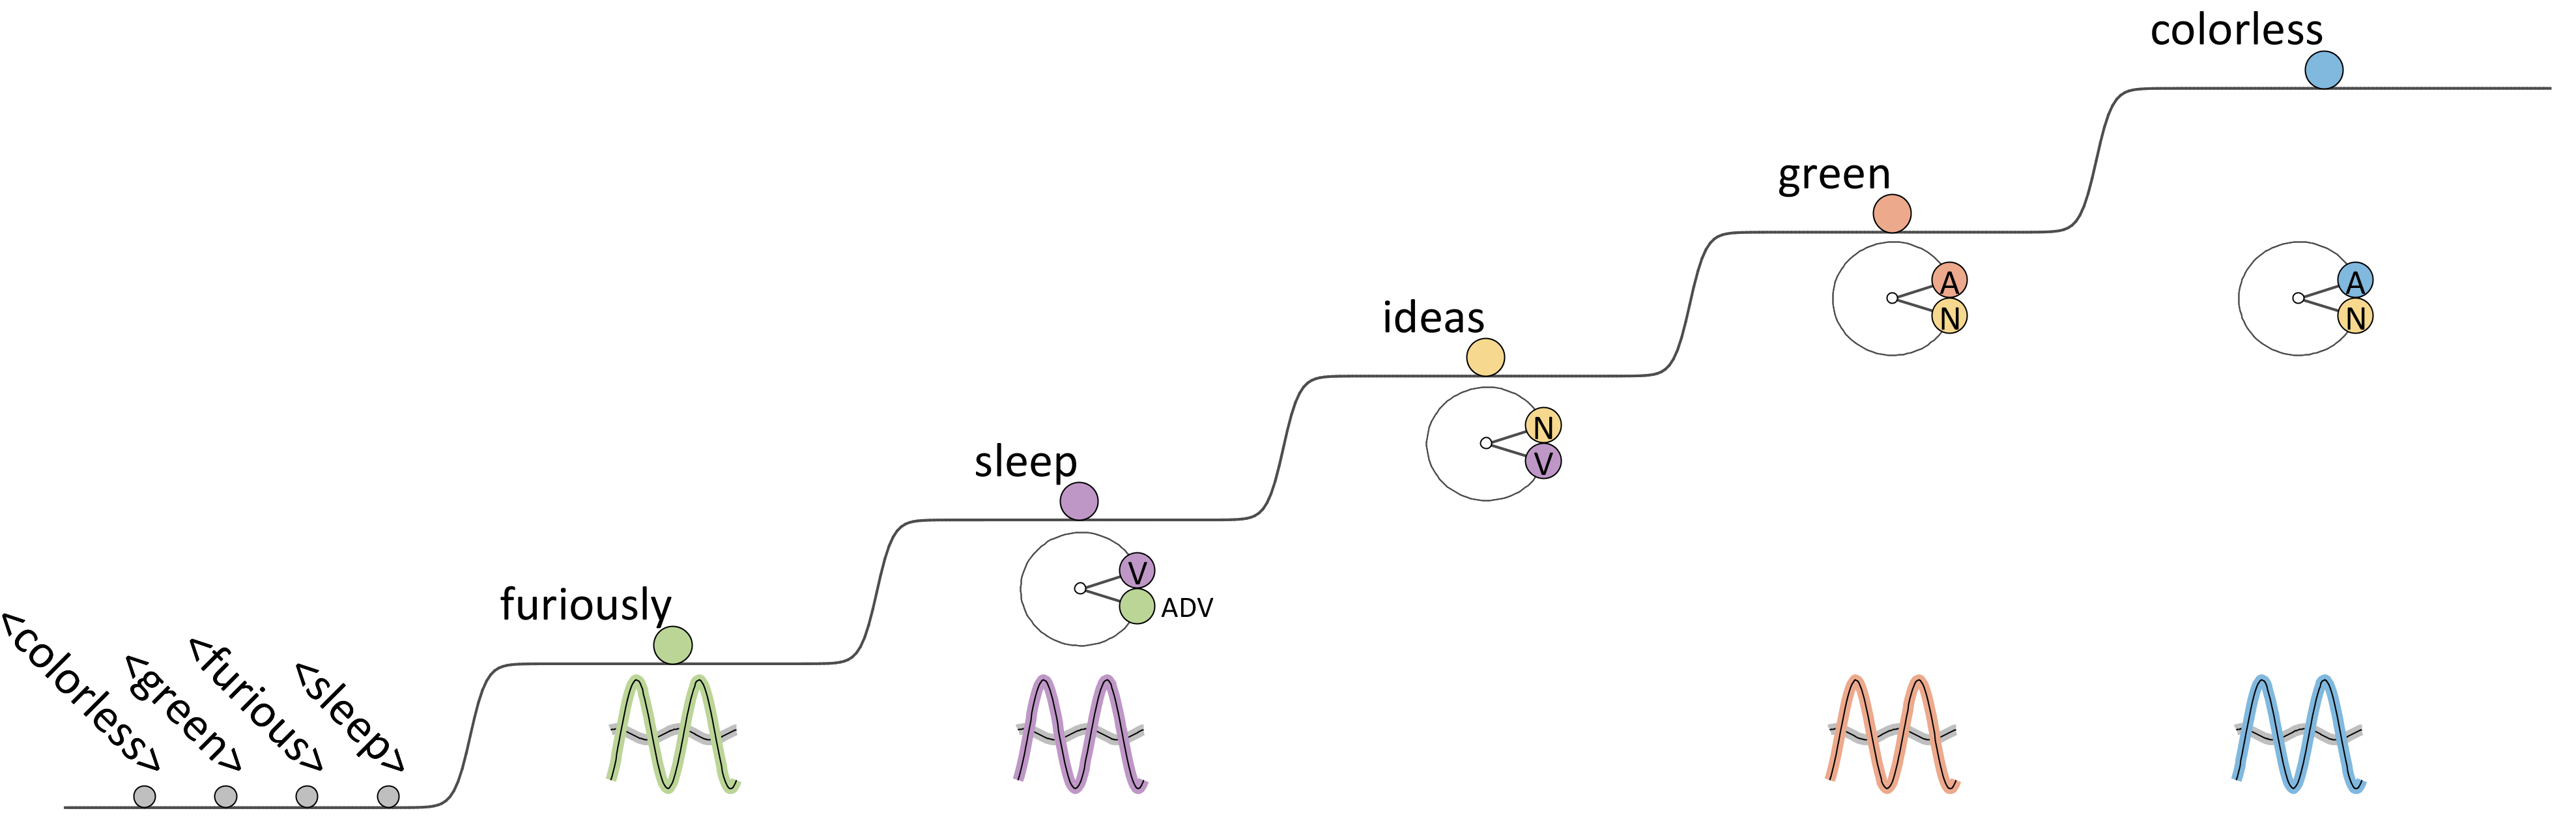
\includegraphics[width=\textwidth]{figures/Tilsen-img134.png}
\caption{Conceptual oddness can arise from many weak interactions between c-sys\-tems.}
\label{fig:6:15}
\end{figure}
 

  We might furthermore posit that these weak interactions between <green> and <colorless> are somewhat stronger because there is more population overlap/\isi{interference} between more similar c-sys\-tems: c-sys\-tems associated with a commonly excited superordinate population like [\textsc{color}] may interact more\linebreak strongly than c-sys\-tems which are not associated with a superordinate population, like [coffee] and [toothpaste]. The integrated effects of the <green>-<color\-less> interactions may cause the experience of semantic oddness. Although a more detailed understanding of the experience is desirable, we infer it does not result from \isi{interference} caused by \isi{s-sys\-tem differentiation}.

  Many questions remain open regarding the factors which influence \isi{coherence}. Although we have only scratched the surface of many issues, the o/el framework provides a useful basis for investigating intuitions as experiences. Importantly, we have rejected the distinction between \isi{grammaticality} and \isi{acceptability}. Our analysis of \isi{grammatical coherence} has focused primarily on how \isi{coherence} arises in interpretation. Another relevant question is whether coherent trajectories necessarily arise in production. Perhaps an invariant, stable ϕ-con\-fi\-gu\-ra\-tion arises in both production and interpretation, despite the lack of constraint on initial conditions. This similarity between production and interpretation is represented in {\figref{fig:6:16}}.

  
\begin{figure}
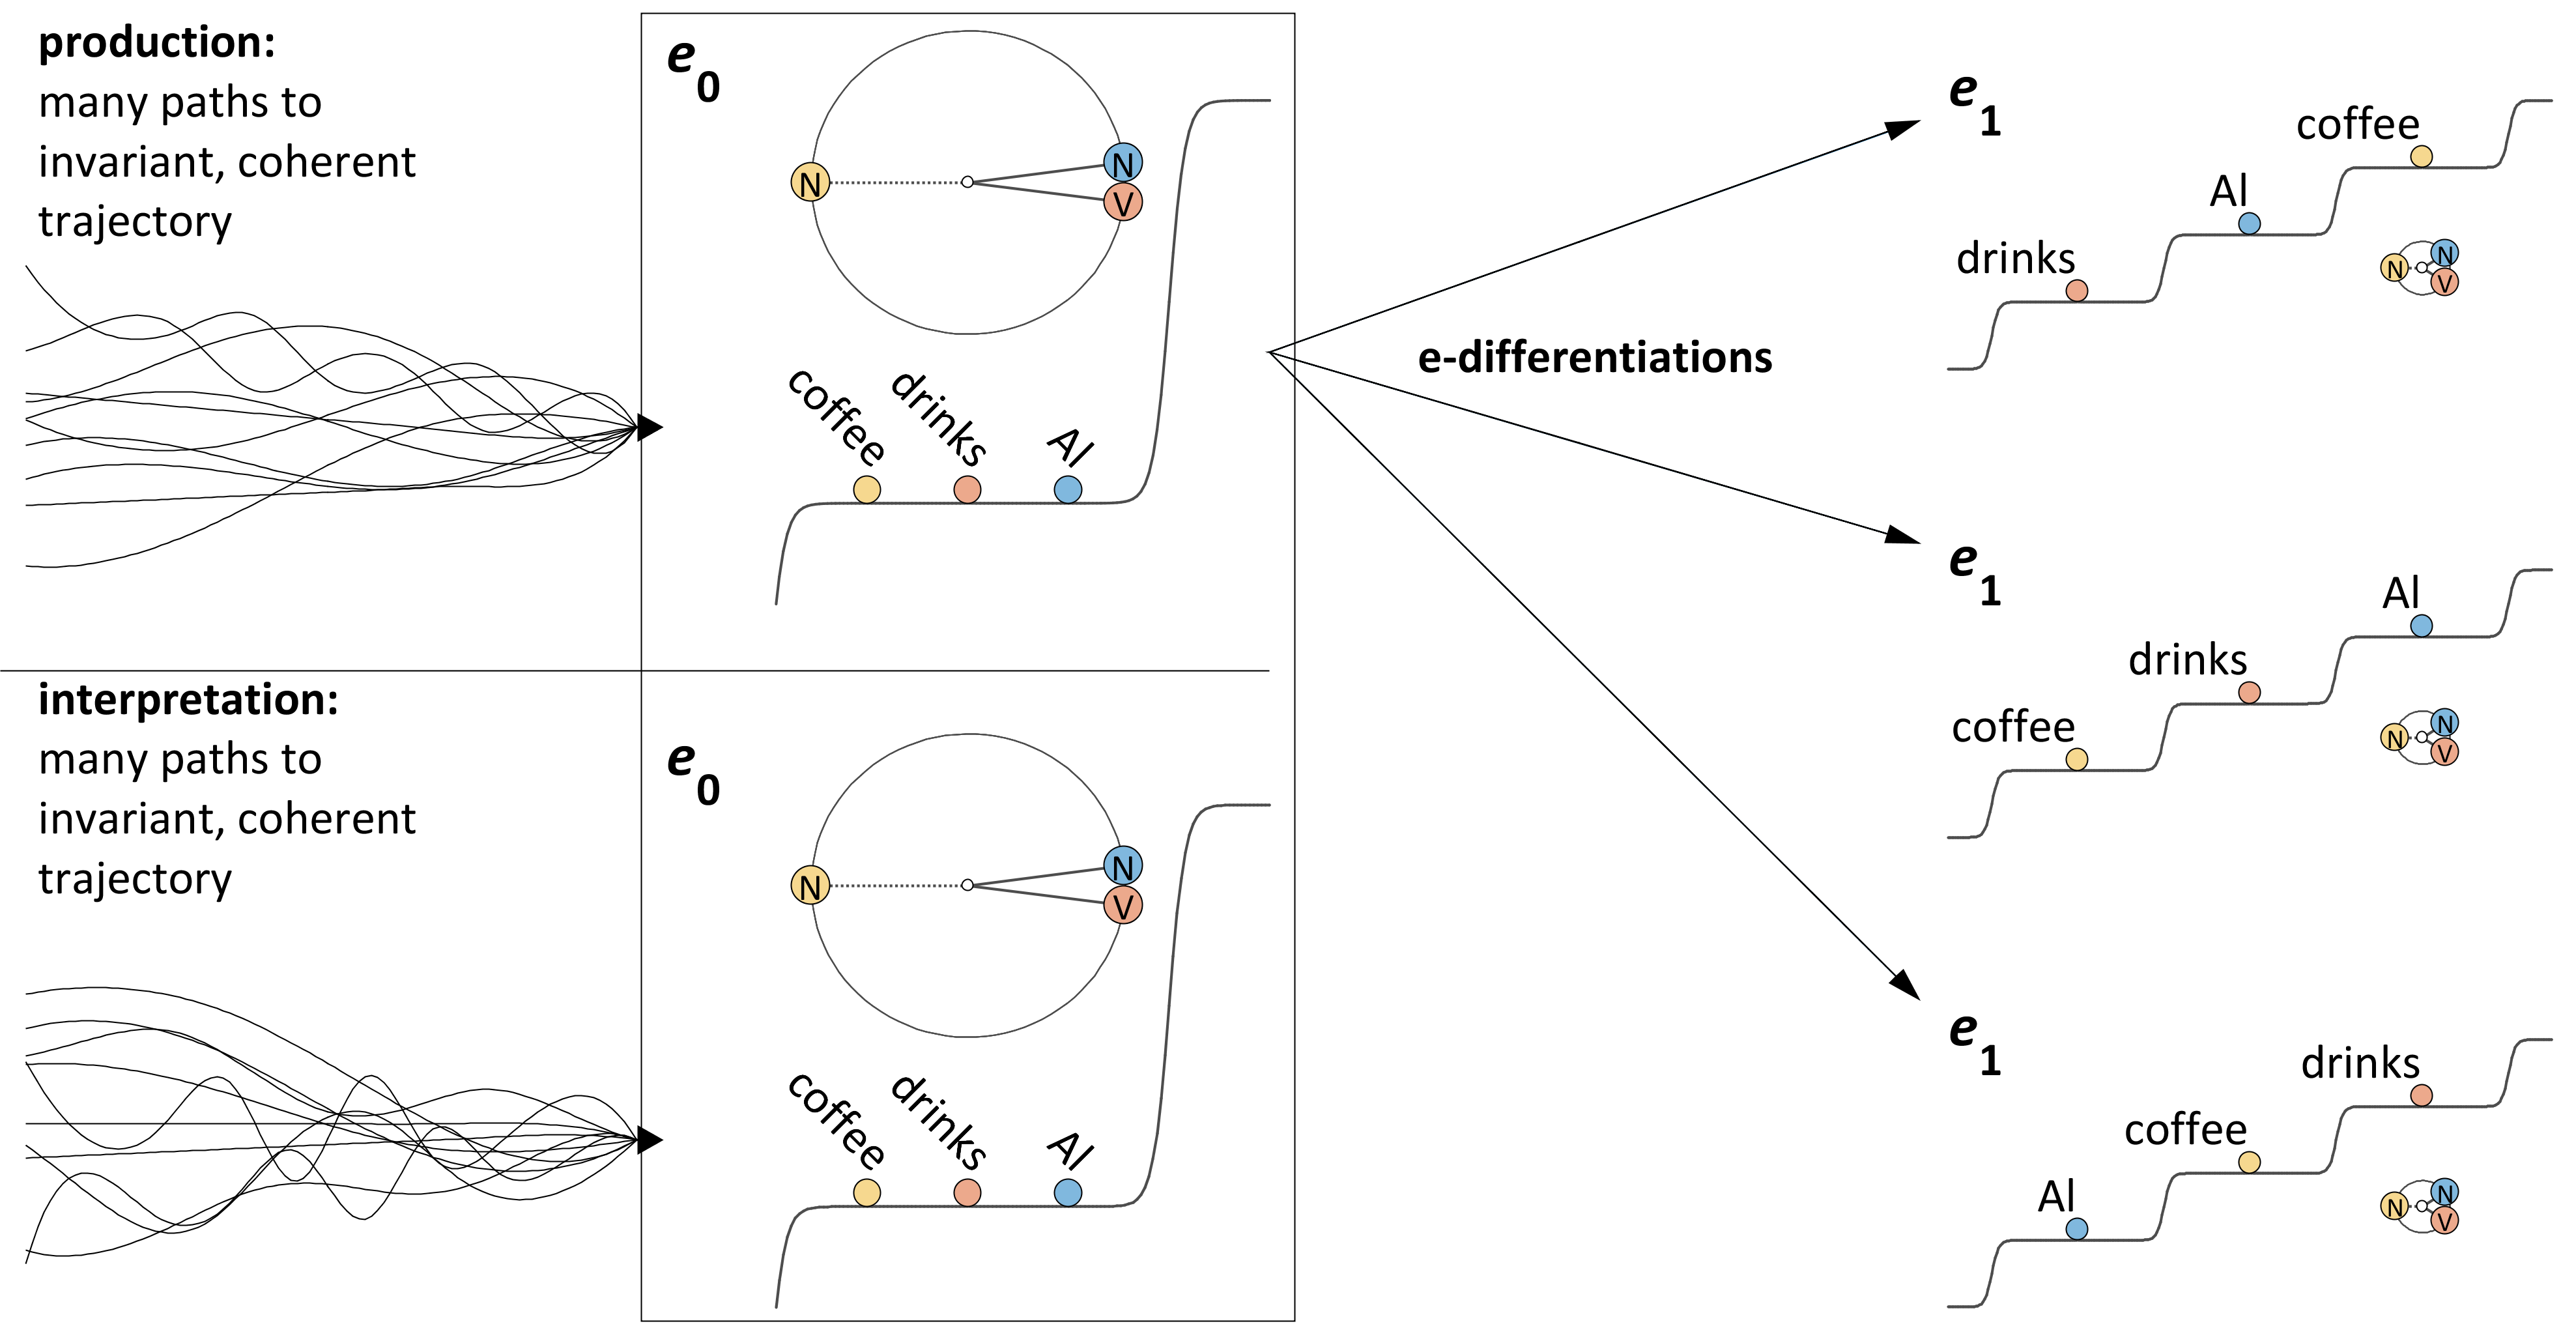
\includegraphics[width=\textwidth]{figures/Tilsen-img135.png}
\caption{Production and interpretation trajectories exhibit a local increase in order.}
\label{fig:6:16}
\end{figure}
 

  Production and interpretation are similar in that there are many possible initial states which may evolve toward the same locally invariant ϕ-con\-fi\-gu\-ra\-tion. In production, variation in e-or\-ga\-ni\-za\-tion can be used to select cs-sys\-tems in different orders (constrained by language-specific ϕ-e mappings), and yet all of these will evoke the same invariant ϕ-con\-fi\-gu\-ra\-tion for an \isi{interpreter}. It is important to consider that both production and interpretation involve local increases in order. The local concentration of order only occurs when a system has work done on it by the \isi{surroundings}; hence we deduce that both production and interpretation are driven by \isi{surroundings} forces. Microscopically, these forces are presumably manifested from electrochemical gradients that the nervous system functions to maintain. In other words, \isi{coherence} is possible because the microscale system self-organizes to a state in which macroscopic, coherent, ordered patterns arise.

\subsection{Constituency intuitions}

What gives rise to intuitions about \isi{constituency}, i.e. about how words are group\-ed, or organized? For example, in the utterance \textit{Al drinks the cold coffee}, we experience an intuition that the words \textit{the cold coffee} constitute a “group” in a way that the words \textit{the cold} do not. In conventional terminology, \textit{the cold coffee} is a constituent, while \textit{the cold} is not a constituent. But what does it mean for words to “be grouped” or to “form a unit” when our conceptual model has no object-like units, and thus no connection or containment of units? Here we show how we can understand these sorts of intuitions through analysis of \isi{coherence}. Note that viewing \isi{constituency} as intuitional rather than configurational (i.e. as a particular class of substate) is consistent with the observation that many ordering phenomena are not amenable to constituency-based analysis (\citealt{Langacker1997,Phillips2003}).

  Conventional \isi{phrase structure} grammars account for \isi{constituency} intuitions with the connection/\isi{containment blend} whereby a node contains all of the nodes which are below it and connected directly or indirectly to it. Thus in the schema in {\figref{fig:6:17}}, \textit{the cold} is not a constituent because there is no node which contains exactly those syntactic objects -- the DP node also contains \textit{coffee}. An additional constraint that non-trivial constituents must correspond to a \isi{phrasal node} can be imposed, so that terminal elements such as \textit{coffee}, \textit{the}, or \textit{cold} are only constituents in a vacuous sense. 

  
\begin{figure}
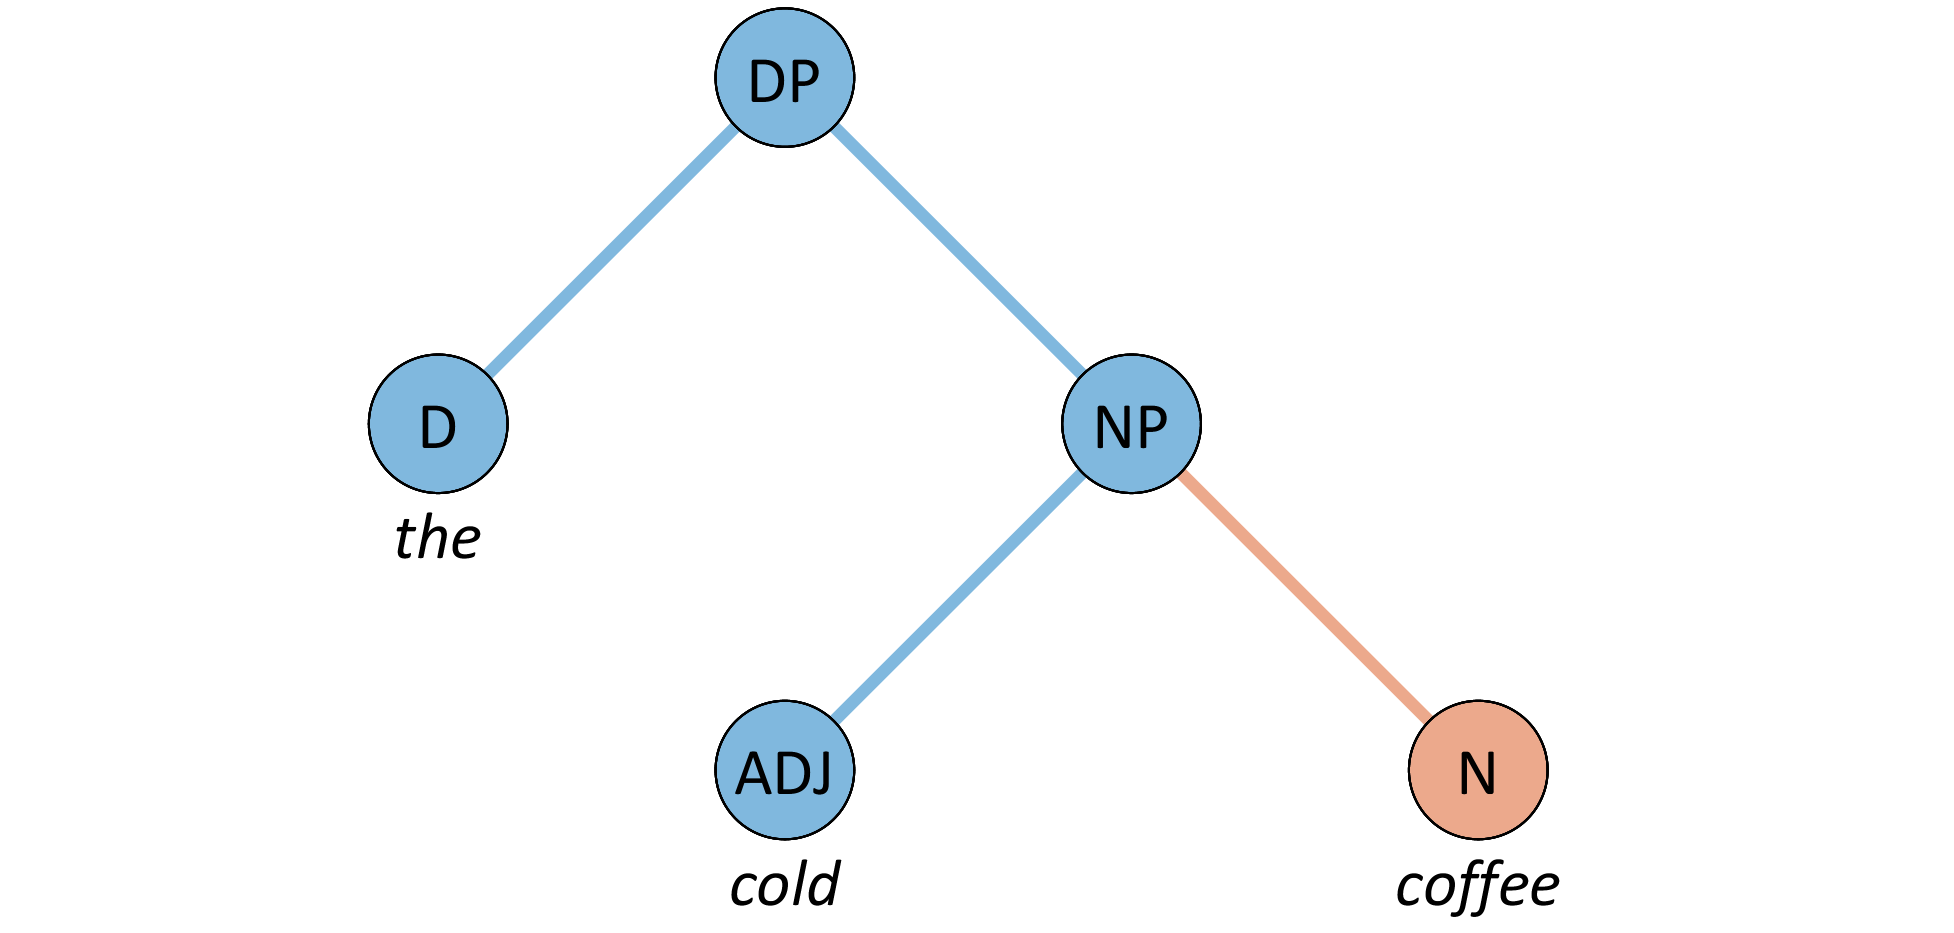
\includegraphics[width=.75\textwidth]{figures/Tilsen-img136.png}
\caption{Orientation and connection patterns are the basis for constituency in conventional frameworks.}
\label{fig:6:17}
\end{figure}
 

  Our intuitions about constituents are associated with \isi{constituency} “tests”,\linebreak some of which are exemplified in {\tabref{tab:6:2}} (cf. \citealt{Carnie2013,Ouhalla1999} for more comprehensive introductions). Note that these tests are less applicable to verb phrase \isi{constituency} and some other sorts of constituents; our focus here is on determiner-adjective-noun constituents.

\begin{table}
\begin{tabularx}{\textwidth}{lQQ}
\lsptoprule
\multicolumn{3}{c}{ ψ\textsubscript{0} : \textit{Al drinks the cold coffee}}\\
\multicolumn{1}{c}{ψ\textsubscript{CT}:} & $\varepsilon $\textit{: \textit{the cold coffee}} & $\varepsilon $\textit{: the cold}\\
\midrule 
\raggedleft \isi{topicalization} & \textbf{The cold coffee}, Al drinks. & \textbf{The cold}, Al drinks coffee.\\
\raggedleft passive & \textbf{The cold coffee} was drunk by Al & \textbf{The cold} was drunk coffee by Al\\
\raggedleft cleft & It is \textbf{the cold coffee} that Al drinks. & It is \textbf{the cold} that Al drinks coffee.\\
\raggedleft \isi{pseudocleft} & \textbf{The cold coffee} is what Al drinks. & \textbf{The cold} is what Al drinks coffee.\\
\lspbottomrule
\end{tabularx}
\caption{Noun phrase constituency tests.}\label{tab:6:3}
\label{tab:6:2}
\end{table}
  The general procedure for conducting a \isi{constituency} test is as follows. First, a candidate set of words $\varepsilon $ is chosen from a base sentence, which in o/el terms is a trajectory ψ\textsubscript{0} in which cs-sys\-tems associated with $\varepsilon $ are selected. The trajectory is typically comprised of temporally contiguous e-epochs. In o/el terms this means that the trajectory is not interrupted by intervening epochs in which no systems are selected or in which systems other than $\varepsilon $ are selected. Indeed, $\varepsilon $ corresponds to a subpart of the trajectory ψ\textsubscript{0} in a subspace of the system. The test is applied by constructing a test sentence (i.e. trajectory) ψ\textsubscript{CT}, according to some particular pattern (e.g. \isi{topicalization}, passivization, etc.). \isi{Grammaticality}/\isi{acceptability} (i.e. \isi{coherence}) intuitions evoked from the sentence are then assessed to infer \isi{constituency}. 

  In the case of the \isi{topicalization} test, ψ\textsubscript{CT} is a trajectory in which the candidate $\varepsilon $ is the first part of the selectional phase of ψ\textsubscript{CT}. The \isi{coherence} intuitions that arise from this procedure for a variety of $\varepsilon $ are represented in \REF{ex:6:22}. The only $\varepsilon $ which does not induce a relatively non-coherent experience is \textit{the cold coffee}, and according to conventional analyses this is because these words exactly correspond to the words contained in a \isi{phrasal node}. The conventional analysis of the \isi{topicalization} test is somewhat unsatisfying because \textit{cold coffee} could also correspond to a \isi{phrasal node} (depending on various analytic choices) but nonetheless fails the test; further stipulations are necessary to explain why the \isi{topicalization} pattern cannot apply to \textit{cold coffee}.

\ea\label{ex:6:22}
  \ea[]{the cold coffee, Al drinks.}
  \ex[*]{the cold, Al drinks coffee.}
  \ex[*]{the, Al drinks cold coffee.}
  \ex[*]{coffee, Al drinks the cold.}
  \ex[*]{cold coffee, Al drinks the.}
  \z
\z

  The o/el re-analysis of \isi{constituency} begins with a subtle but important point: we do not have intuitions about \isi{constituency} until we interpret a potential constituent in some other context. More technically, \isi{constituency} intuitions are \textit{always} associated with the \isi{coherence} of interpretation of a sub-part of a coherent trajectory, when that subpart is interposed in another trajectory. There are no “\isi{constituency} intuitions” until we engage in a particular mode of interpretation which involves these metalinguistic trajectory manipulations. This conception not only leads to a new, useful understanding of \isi{constituency}, based on the notion of \isi{coherence}, but also explains why \isi{constituency} intuitions do not accord with \isi{acceptability} for patterns of \isi{ellipsis} and \isi{anaphora}, which we examine in detail in the next chapter. To illustrate, consider the following reference trajectory ψ\textsubscript{0}, of \textit{Al drinks the cold coffee}:

  
\begin{figure}
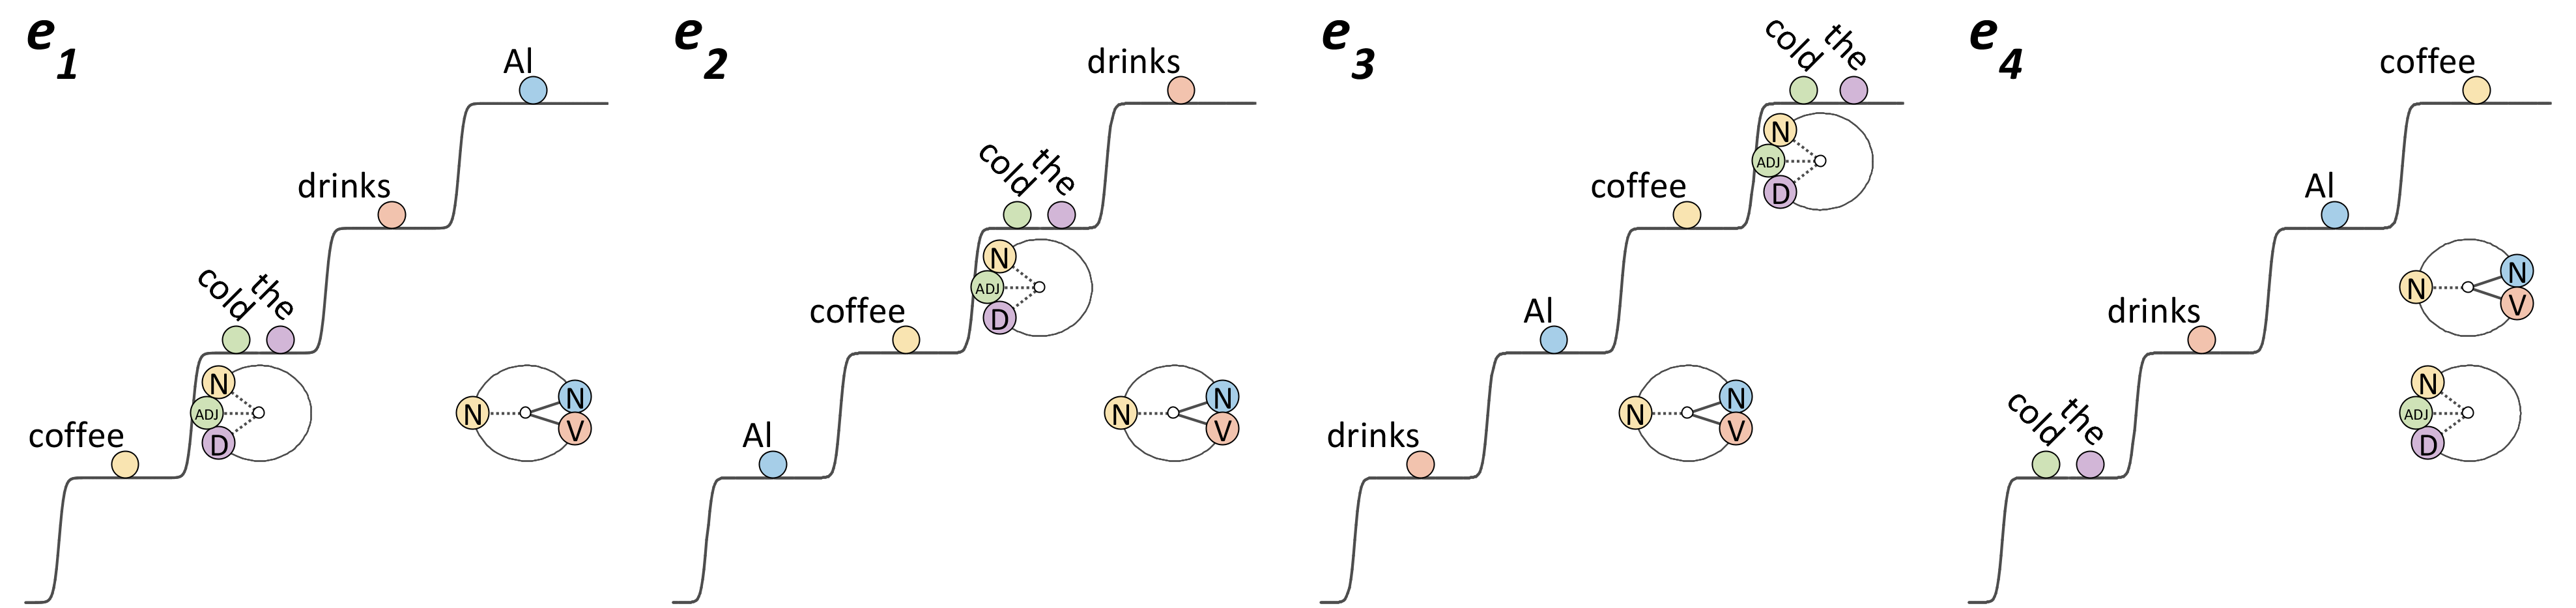
\includegraphics[width=\textwidth]{figures/Tilsen-img137.png}
\caption{Reference trajectory for constituency tests: \textit{Al drinks the cold coffee.}}
\label{fig:6:18}
\end{figure}
  

  To assess the \isi{constituency} intuition for \textit{the cold coffee}, we identify the trajectory in {\figref{fig:6:18}} of epochs (e3--e4), in which [the]\{D\}, [cold]\{A\textsc{dj}\}, and [coffee]\{N\} are selected. We construct the candidate trajectory $\varepsilon $ by ignoring \isi{state space} dimensions associated with other non-test systems in (e3--e4), i.e. dimensions related to [Al]\{N\} and [drinks]\{V\}. However, we take note of the ϕ-con\-fi\-gu\-ra\-tions which involve the test systems and non-test systems, since we attempt to integrate these with the \isi{constituency} \isi{test trajectory} ψ\textsubscript{CT}. We then construct ψ\textsubscript{CT}, by combining $\varepsilon $ and ψ\textsubscript{CT} according to a desired pattern. This construction procedure predetermines which patterns are suitable (e.g. \isi{topicalization}, clefting, passive, \isi{pseudocleft}). Patterns which omit or replace $\varepsilon $ (i.e. \isi{ellipsis}, \isi{anaphora}) lead to different intuitions about grouping, as does coordination.

  A \isi{test trajectory} for \isi{topicalization} of the candidate \textit{the cold coffee} is shown in {\figref{fig:6:19}}. Although \isi{immediate organization} of [coffee]\{N\} with a \{V\} system is not possible after (e1), excitation of [drinks]\{V\} in (e3) allows [coffee]\{N\} to participate in a ϕ-con\-fi\-gu\-ra\-tion. We can further hypothesize that after epochs of initial system excitation (e1--e3), a coherent \isi{reiterative simulation} (e3, e3′) can arise, in which \isi{utterance coherence} criteria are met. This analysis entails that \isi{constituency} intuitions arise from experiencing the achievement of a coherent trajectory, and not necessarily from an experience of the path that is taken to achieve that trajectory.

  
\begin{figure}
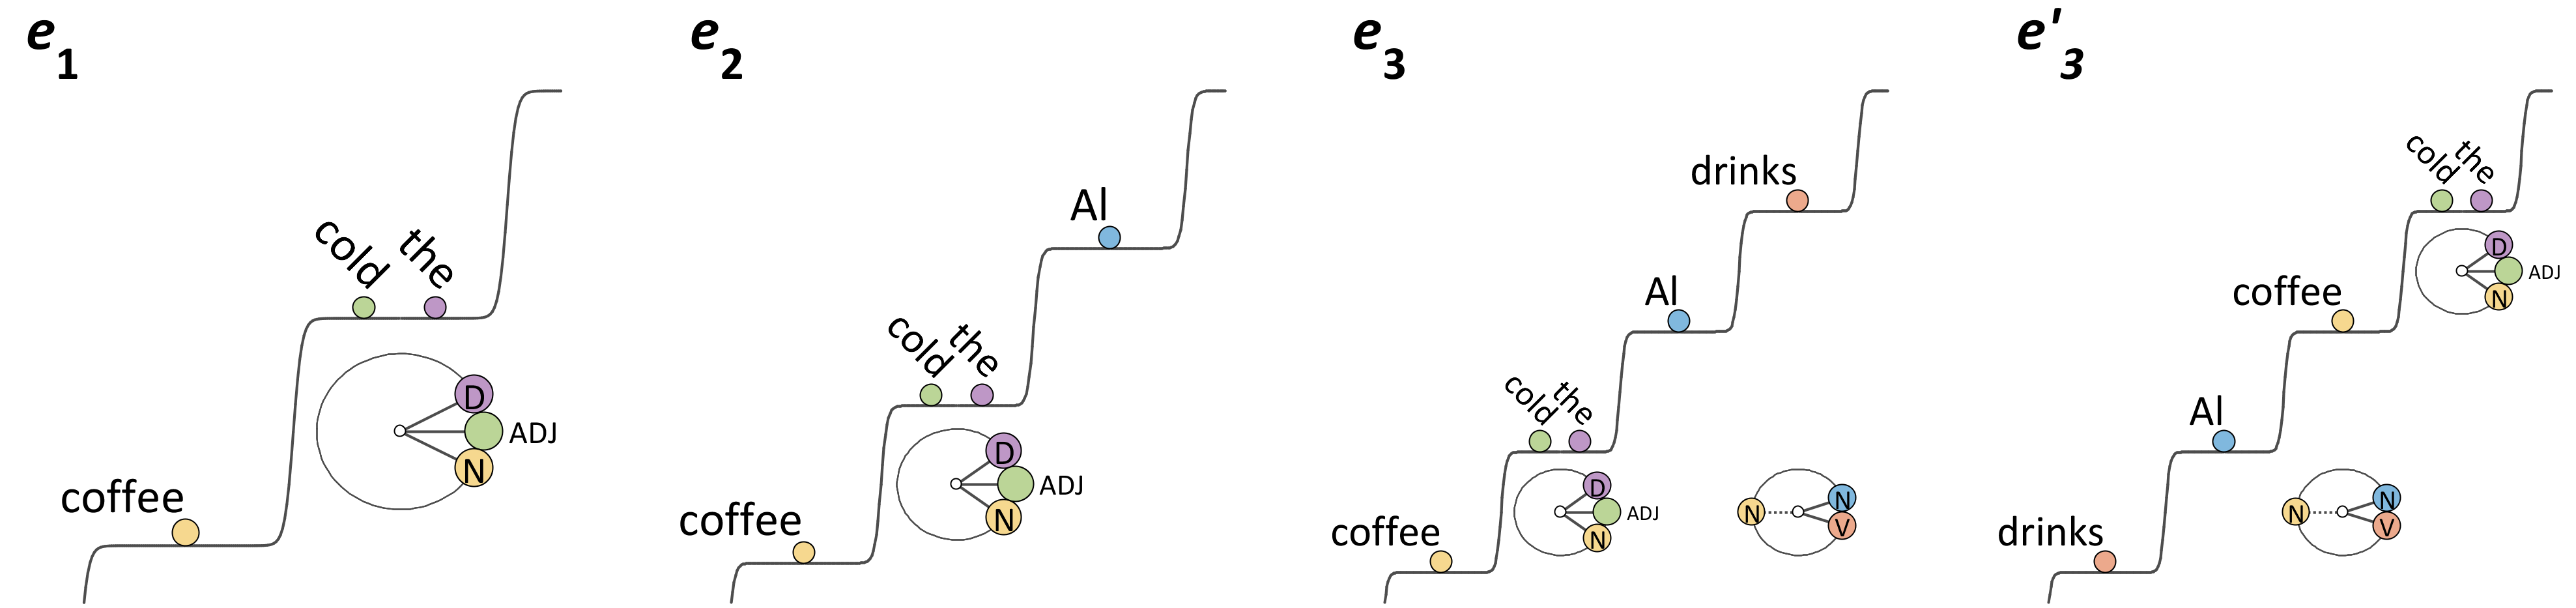
\includegraphics[width=\textwidth]{figures/Tilsen-img138.png}
\caption{Topicalization test trajectory for constituency of \textit{the cold coffee}.}
\label{fig:6:19}
\end{figure}
 

  In contrast to \textit{the cold coffee}, the \isi{topicalization} test of \textit{the cold} does not lead to a coherent state. The likely reason is shown in {\figref{fig:6:20}}: neither [cold]\{A\textsc{dj}\} nor [the]\{D\} can ϕ-couple to the lexical \{N\} system [coffee]\{N\}, which is necessary for the expected ϕ-con\-fi\-gu\-ra\-tions of \{A\textsc{dj}\} and \{D\}. This raises the question of why in (e4) [the]\{D\} and [cold]\{A\textsc{dj}\} cannot couple to [coffee]\{N\} and thus give rise to the ϕ-con\-fi\-gu\-ra\-tion required for \isi{coherence}. One possibility is that the \isi{immediate organization bias} is stronger for \{D\} and \{A\textsc{dj}\} systems than for \{N\} systems. It may be more difficult to maintain \{D\} and \{A\textsc{dj}\} systems in an unstable state across multiple epochs than it is to maintain \{N\} systems.

  
\begin{figure}
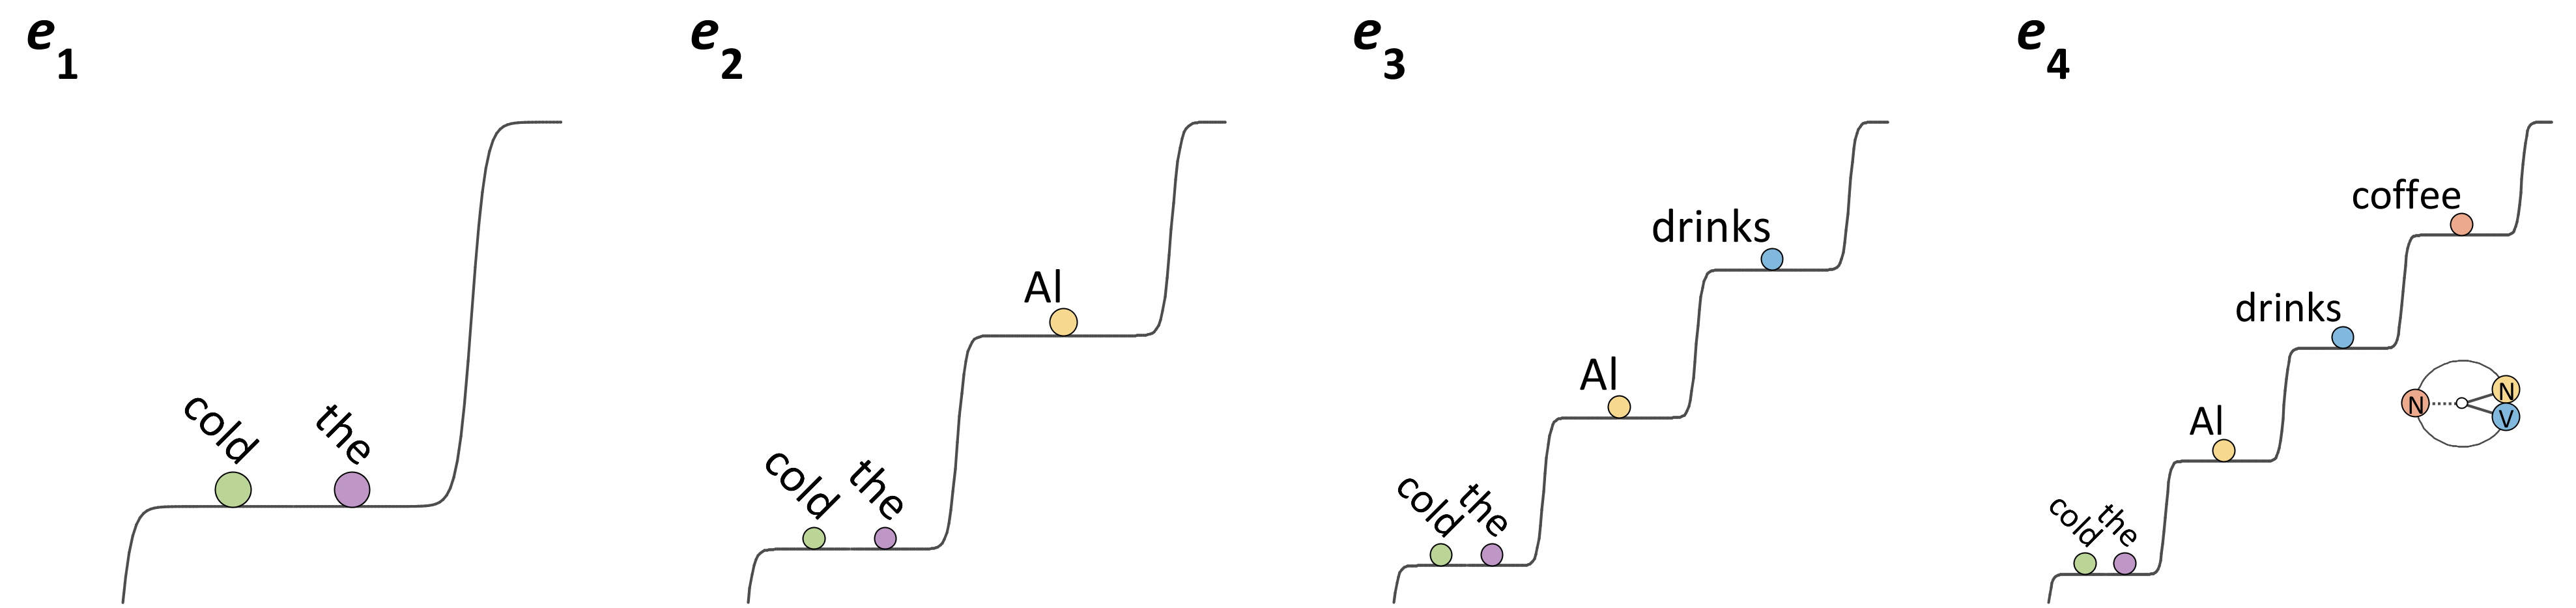
\includegraphics[width=\textwidth]{figures/Tilsen-img139.png}
\caption{Topicalization test trajectory for a non-constituent does not lead to a coherent state.}
\label{fig:6:20}
\end{figure}
 

  Similar accounts can be extended to passivization, \isi{pseudocleft} and cleft tests, shown in {\figref{fig:6:21}}. The grayed ϕ-con\-fi\-gu\-ra\-tions with \{D\} and \{A\textsc{dj}\} are ones which, because of the intervening epochs, are unable to participate in the expected configuration. There may be other reasons why \isi{coherence} does not occur in these examples. For instance, [cold] might couple to an \{N\} system, which allows for \isi{immediate organization} with [is]\{A\textsc{ux}\} in all three examples. In the cleft, [cold] might couple with [Al]\{N\}, in which case [drinks]\{V\} would have no \{N\} system to +ϕ couple with because [Al]\{N\} couples with [is]\{A\textsc{ux}\}. Thus the \isi{immediate organization bias} may be an important factor in determining the \isi{coherence} intuitions associated with \isi{constituency}.   

  
\begin{figure}
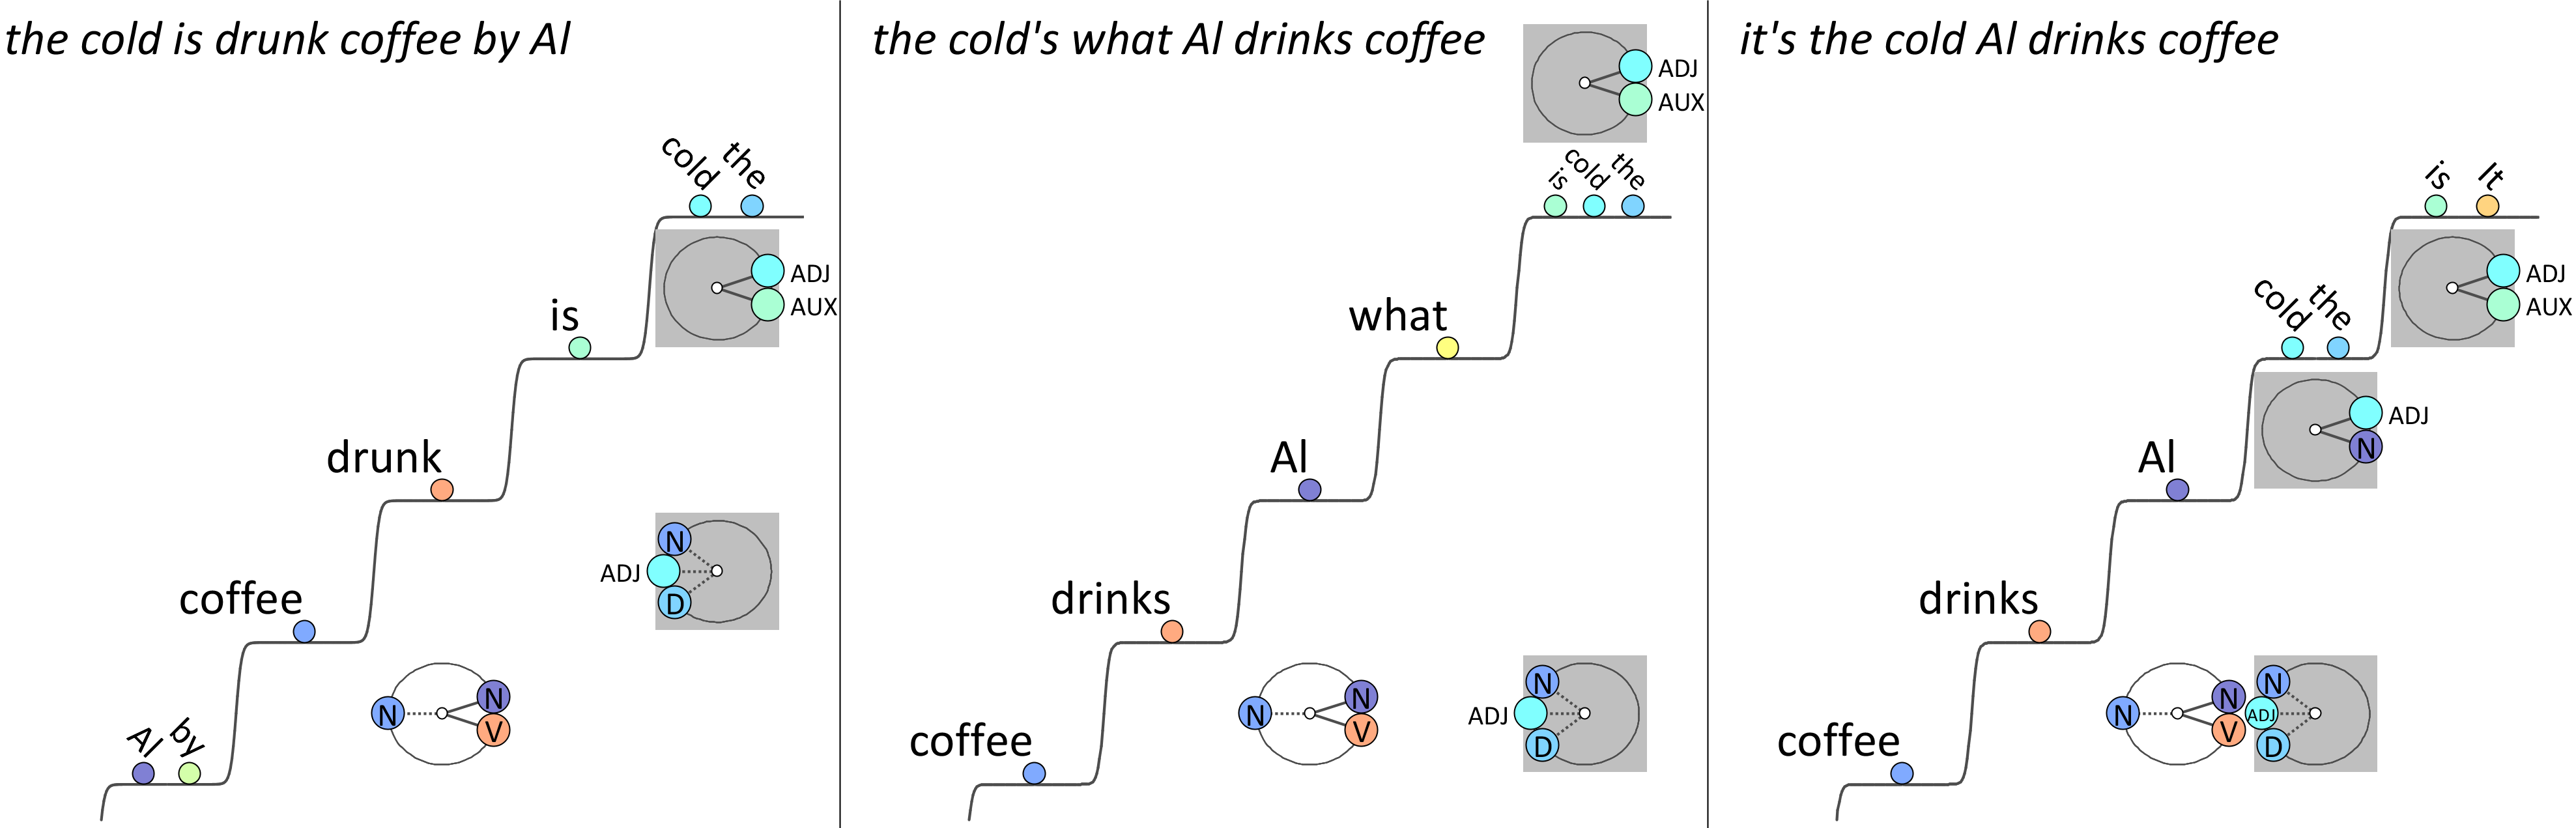
\includegraphics[width=\textwidth]{figures/Tilsen-img140.png}
\caption{Non-coherence in passive, cleft, and pseudocleft constituency tests.}
\label{fig:6:21}
\end{figure}
 

  There may be a variety of additional reasons why \isi{coherence} is not achieved when some particular ψ\textsubscript{CT} is constructed, and a more comprehensive analysis is desirable, one which could predict when \isi{coherence} is expected in a broader range of \isi{constituency} tests. The o/el framework nonetheless brings us some clarity by discouraging us from thinking of “constituents” as objects; instead, we reconceptualize \isi{constituency} as a phenomenon which derives from experiences of \isi{coherence} or the lack thereof. This requires us to refocus our investigations of \isi{constituency} phenomena on temporal patterns in interpretation, as opposed to \isi{atemporal}, abstract structural relations.

\section{Electrophysiological and behavioral manifestations of coherence}

Grammatical \isi{coherence} on the utterance scale depends on epoch scale \isi{coherence}, which in turn depends on auto-spectral and cross-\isi{spectral coherence} of excited c- and s-sys\-tems. Thus \isi{spectral coherence} is the fundamental basis for many aspects of \isi{grammaticality} intuitions. Here we show how \isi{spectral coherence} can be related to electrophysiological and behavioral phenomena, specifically focusing on event-related potentials (ERPs) in sentence processing. In order to accomplish this, we first develop a set of linking hypotheses. The \isi{coherence} phenomena analyzed below are assumed to occur before the \isi{reiterative} trajectories which are necessary for \isi{grammatical coherence}; intuitions regarding \isi{grammatical coherence} are dependent on and arise subsequently to the electrophysiological manifestations of \isi{spectral coherence}. By means of its emphasis on \isi{coherence}, the o/el framework provides an alternative vocabulary for understanding various \isi{psycholinguistic} phenomena.

\subsection{Linking hypotheses for spectral coherence}

One of the major methodological instruments used to study syntactic and conceptual processing is electroencephalography (EEG). EEG measures voltage fluctuations generated by neural spiking in the brain, using electrodes placed on the scalp. When EEG signals are aligned to the time at which a stimulus is presented, changes in measured voltages are observed -- these are called event-related potentials (ERPs). A number of different ERP patterns have been identified. These are hypothesized to be associated with syntactic and/or semantic “processing,” a concept which we reinterpret in the current framework. ERPs are commonly given names which refer to when and/or where they are observed, along with whether the observed voltages are negative or positive relative to a reference voltage. For example, researchers have identified an “\isi{N400}” which is a negative voltage change that occurs in association with semantic processing, a “\isi{P600}” which is a positive voltage change that occurs in association with syntactic and/or conceptual reanalysis (as in the interpretation of \isi{garden path} sentences), and an “ELAN” (early left anterior negativity) which is associated with \isi{syntactic category} processing. 

Here we develop a set of linking hypotheses which allow for the o/el model to generate ERP patterns that are in some ways qualitatively similar to observed ERPs. The key idea behind this approach is that “processing” -- a rather vague term -- can be reinterpreted more mechanistically as change in the auto-\isi{spectral coherence} of c- and s-sys\-tems, and change in the cross-\isi{spectral coherence} of cs-sys\-tems. For reasons that are made clear below, our focus is on the time-course of such changes as a function of stimuli, rather than their spatial distributions in the brain.

When a single neuron spikes or receives input from other neurons, there is a transmembrane ionic current associated with changes in membrane potential. When the axons of many neurons are oriented similarly in space, the voltage changes associated with individual neurons and synapses combine to create a change in the electrical potential which is measurable above the scalp. Thus the EEG signal is an integration of state changes in many neurons which have similar orientations. Axons of pyramidal cortical neurons generate most of the cortical EEG signal because these are closest to the scalp (\citealt{FedermeierLaszlo2009,KutasDale1997}). The extracellular fluid and cranium act as coarse spatial filters on the signal, and hence the spatial resolution of EEG is poor compared to other measurement techniques such as fMRI. Furthermore, the mathematical problem of localizing the origins of EEG signals in the brain is underdetermined. However, the temporal resolution of EEG is far superior to fMRI and thus it is better suited to investigating the time-course of syntactic/semantic processing. 

Even in the absence of sensory stimuli, the brain exhibits EEG signals with power at a range of frequencies \citep{Buzsaki2006}. These oscillations are thought to provide a basis for interactions between brain areas, and to facilitate processing of sensory stimuli \citep{FriesEtAl2001,GrayEtAl1989}. Event-related potentials (ERPs) are measured by presenting a stimulus and averaging the stimulus time-locked electrical activity over a large number of trials. The assumptions behind this approach are that the electrical response to the stimulus is of fixed polarity and occurs at a fairly consistent latency relative to stimulus presentation \citep{PennyEtAl2002}. The averaging is necessary because there is typically a large amount of neural activity that is not specific to the stimulus (i.e. noise). There are two main theories on the neural origins of event-related potentials (ERPs): the phase resetting (\isi{phase modulation}, PM) theory and the evoked response (amplitude modulation, AM) theory \citep{MakeigEtAl2002,PennyEtAl2002,ShahEtAl2004}.

In the evoked response theory, stimuli “evoke” a neural population response, and EEG power increase is expected in a single trial. Averaging evoked responses over multiple trials amplifies this power increase and thereby produces the ERP pattern. In the phase-resetting theory, sensory stimuli induce a phase-reset of ongoing EEG rhythms. Under this view, the reason the ERP pattern is observed is due to averaging over trials: in a single trial, no increase in neural activity is expected, but the EEG rhythm will be phase-coherent across trials when time-aligned to the stimulus onset; hence averaging over multiple trials is necessary to observe an ERP, which reflects phase-\isi{coherence}. Another possibility is that both phase-modulation and amplitude modulation influence ERPs \citep{PennyEtAl2002,ShahEtAl2004}. For current purposes we assume that both of these effects contribute to \isi{coherence}. 

  Many language-related ERP studies investigate sentence processing by comparing ERPs between conditions in which some relevant syntactic or semantic aspect(s) of sentences are varied. The comparisons are made by aligning EEG signals to the time when a manipulated word is presented in a sentence. It is important to keep in mind that there is an EEG signal response to the presentation of each word in a sentence, and that the response to any given word is often influenced by responses to preceding words. Thus the dynamics of the EEG signal in response to any particular utterance are quite complicated. 

A set of linking hypotheses is necessary to relate power changes in the EEG signal -- (and ultimately, ERPs) -- to \isi{spectral coherence} dynamics in interpretation trajectories. To illustrate these hypotheses we consider c- and s-sys\-tem \isi{coherence} trajectories and their first-derivatives in a canonical \isi{interpretation trajectory} for \textit{Al drinks coffee}, shown in {\figref{fig:6:22}}. As each word is perceived, sensory systems are excited (not shown). The specific pattern of excitation of sensory systems will in general be based on acoustic information of the stimuli (in the case of auditory stimuli) or visual information (in the case of graphemic/orthographic stimuli), but may also be influenced by “top-down” influences from previously excited conceptual and syntactic systems. Note that we have not developed a specific model of sensory systems in the o/el framework -- such systems have generally been subsumed as part of the \isi{surroundings} of c- and s-sys\-tems. Approximately 40-50ms after stimulus onset, active sensory systems begin to exert forces on both c- and s-sys\-tems, causing them to become excited. The particular c- and s-sys\-tems which experience these forces necessarily depend on learned associations between sensory systems and c-/s-sys\-tems. For example, we have learned that the auditory or visual stimulus \textit{Al} excites an \{N\} s-sys\-tem and [Al] c-sys\-tem. Of course, other c- and s-sys\-tems may also be excited by the stimulus, particularly in cases of homophony, and the extent to which a given c- or s-sys\-tem may be excited by a stimulus is conditioned by learning (i.e. supra-utterance scale system evolution) and context (forces from the \isi{surroundings} which evolve on the utterance scale).

  When the sensory systems activated by \textit{Al} begin to activate \{N\} and [Al] systems, those systems begin to evolve toward an active state in which the individual neurons in the relevant populations are collectively oscillating. Thus there will be a transient period of time in which the auto-\isi{spectral coherence} of each system is increasing. Recall that our \isi{microscale conception} of the \isi{coherence process} is that individual neuronal spikes within the population become more predictable and correlated, and on the \isi{macroscale} this results in a narrowing of the power spectrum of the system, i.e. the emergence of a more ordered state. The power spectra of c- and s-sys\-tems at selected points of time are shown in {\figref{fig:6:22}}. Both the widths and peak amplitudes of the spectra are assumed to be related to the \isi{coherence} of the systems; the increase in \isi{coherence} is modeled here with a first-order differential equation:  $\dot{{x}}=-a\left(x-{x}_{\max}\right)$, where $a$ is a fixed growth rate parameter and $x_{\max}$ is an equilibrium which represents a maximal degree of \isi{coherence}. 

  There are several key features of the trajectories to notice. First, although the s-sys\-tems and c-sys\-tems associated with a stimulus are activated at the same time, the c-sys\-tem cannot reach an above-ground state until after the s-sys\-tem does. This reflects the hypothesis that excitation depends on the emergence of a cs-resonance. Second, there is “priming” for both c- and s-sys\-tems. For example, shortly after the \{V\} system is excited, an \{−N\} system is activated. Likewise, shortly after the [drinks] system is excited, a [coffee] system is activated. These priming effects are assumed to be pervasive, particularly for c-sys\-tems: presumably [drinks] activates a large number of c-sys\-tems (e.g. [tea], [whisky], etc.). Note that only priming of [coffee] is shown here in order to avoid visual clutter. A crucial consequence of the priming is that when the \textit{coffee} stimulus does occur, the \{−N\} and [coffee] systems already have some degree of \isi{coherence}, and hence the change in \isi{coherence} that is necessary to reach an above-ground state is smaller. This also results in a shorter period of time from the stimulus onset to the emergence of an above-ground [coffee]\{−N\} system. Finally, e-or\-ga\-ni\-za\-tion operations are shown here to occur after all three cs-sys\-tems have been excited; this aspect of the system trajectory is a somewhat arbitrary choice, rather than a necessity. It is possible that {\textbar}Al drinks{\textbar} could be e-organized in a more incremental fashion, prior to the emergence of the {\textbar}coffee \{−N\}{\textbar} system. 

  
\begin{figure}
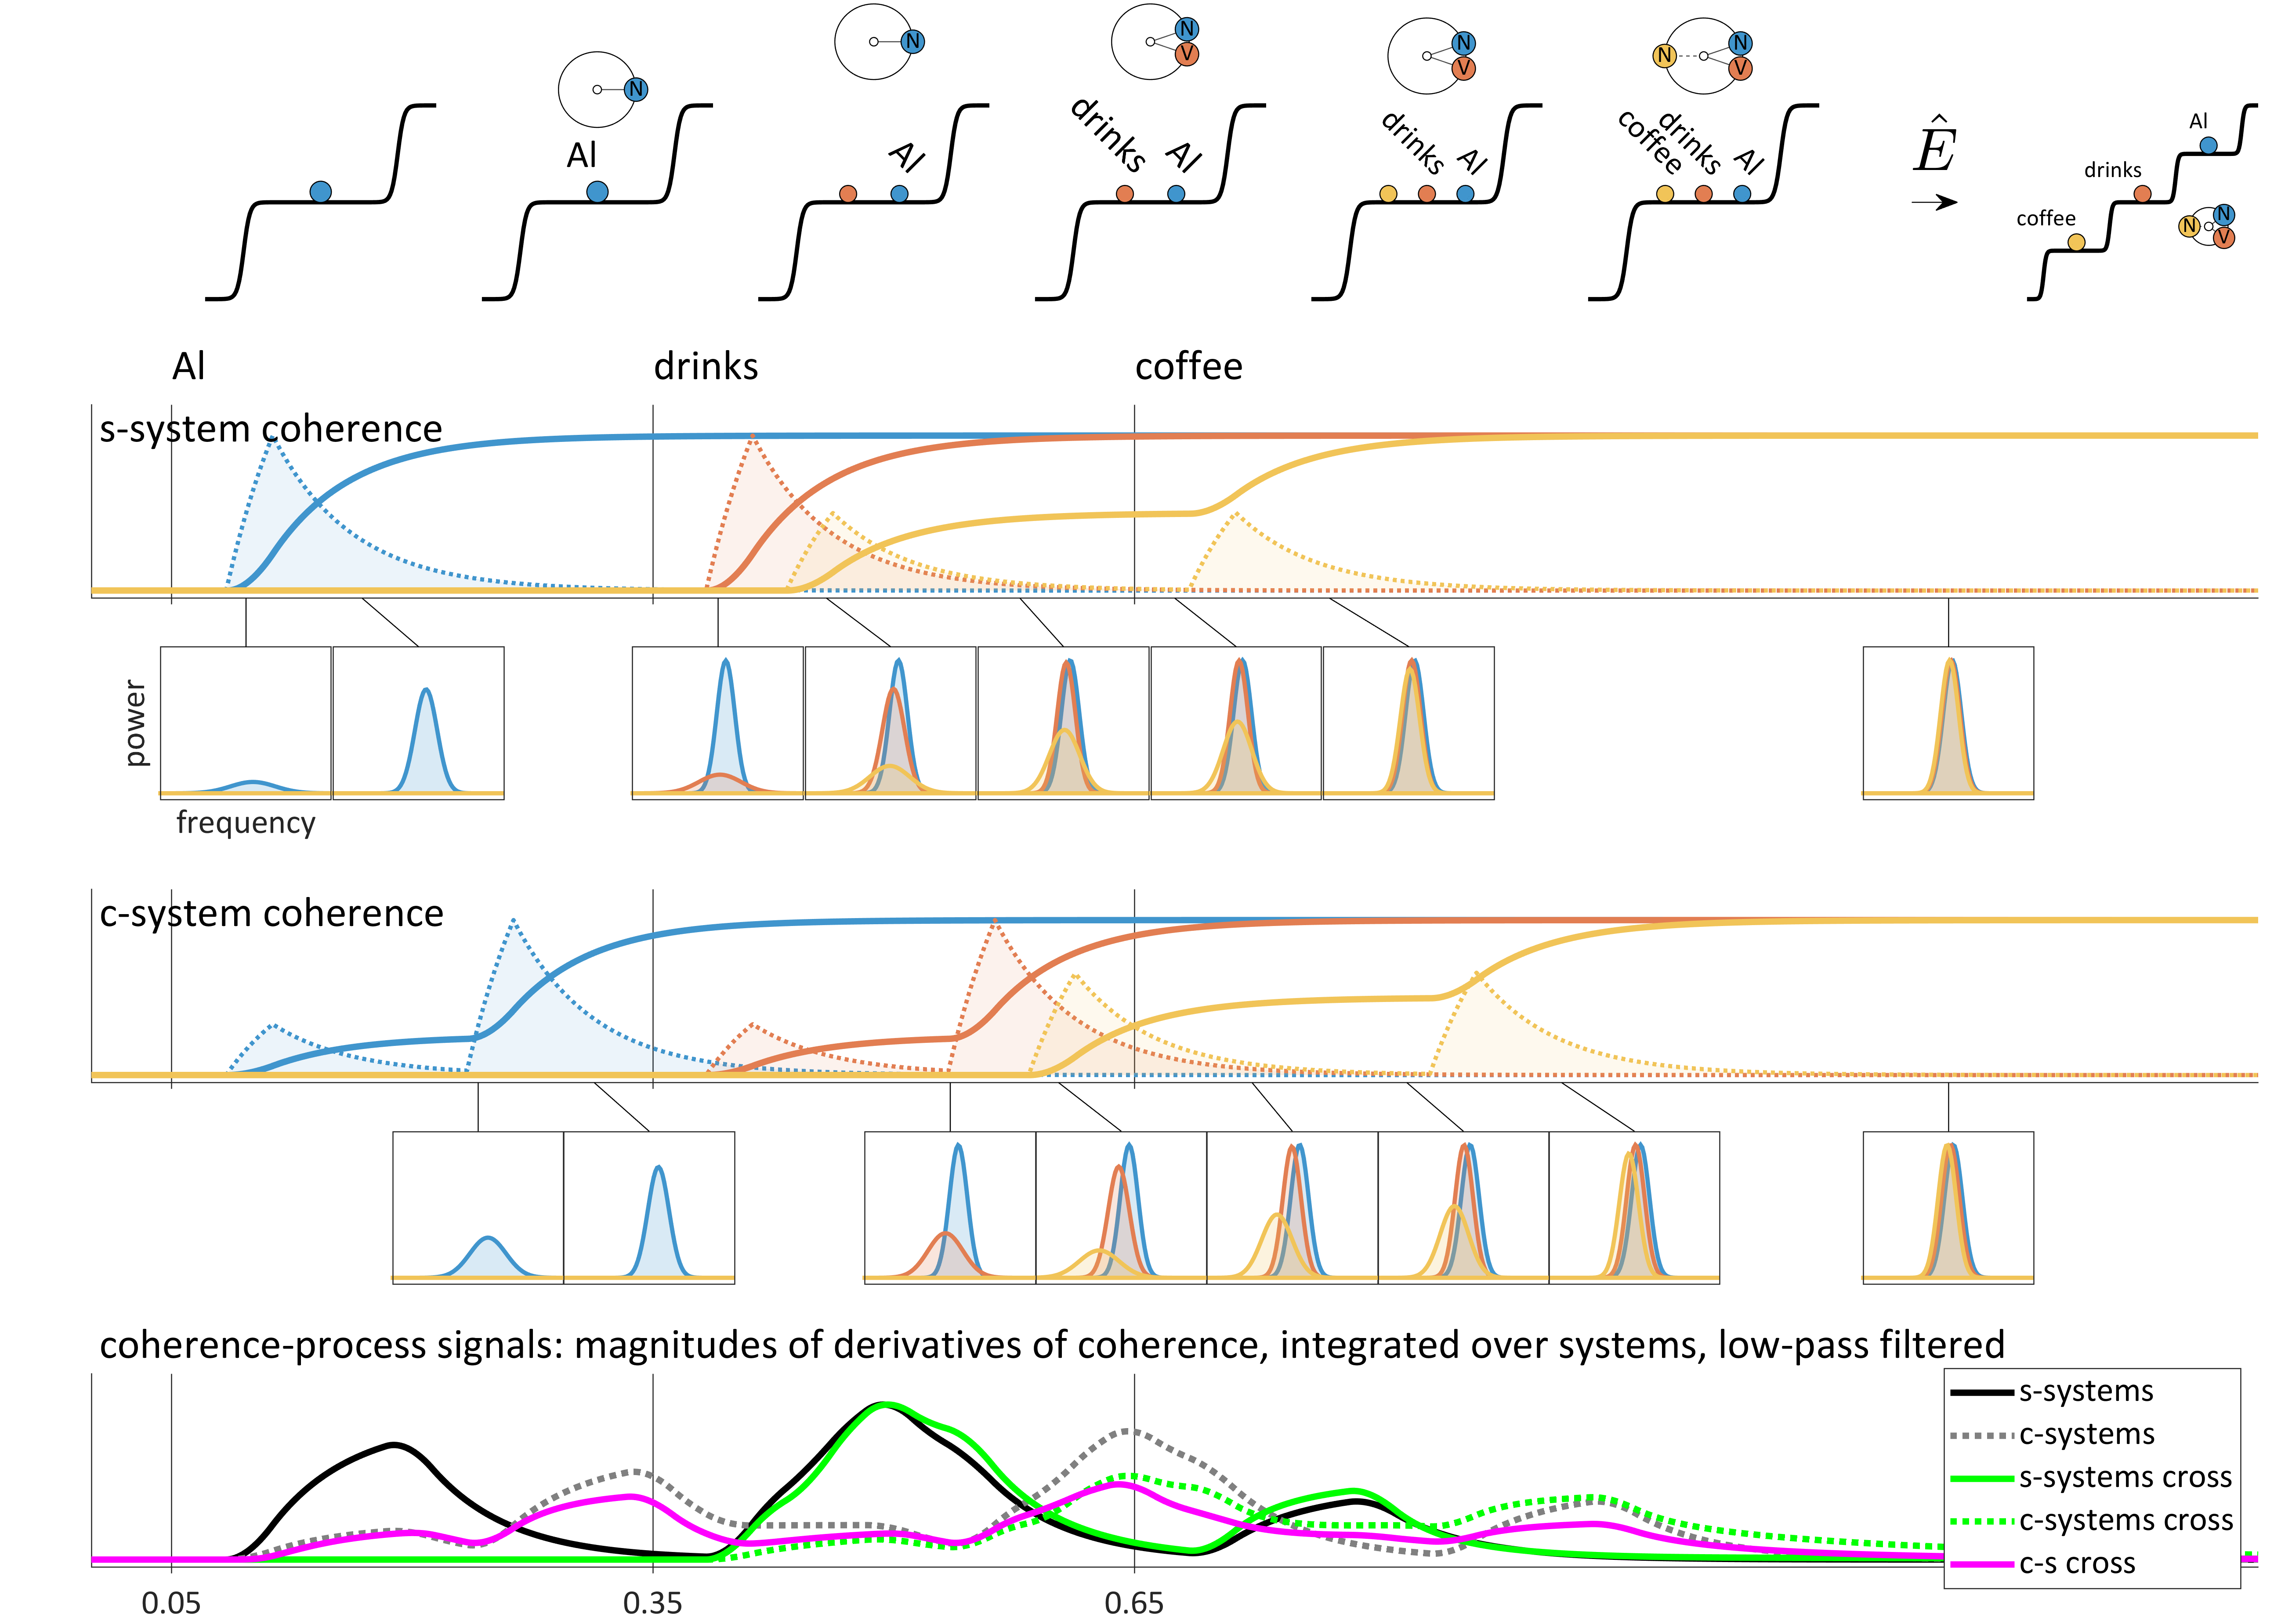
\includegraphics[width=\textwidth]{figures/Tilsen-img141.png}
\caption{Coherence and coherence process signals of s-sys\-tems and c-sys\-tems in an interpretation trajectory.}
\label{fig:6:22}
\end{figure}
 

  The \isi{coherence} trajectories shown for s-sys\-tems and c-sys\-tems above can be used to generate ERPs. Specifically, a short-time integration of the magnitude of the rate of change of \isi{coherence} is hypothesized to correlate with power of the EEG signal. We emphasize that it is the \textit{magnitude of the rate of change of spectral coherence}, rather than \isi{coherence} itself, which is the relevant predictor. This follows from reasoning about how \isi{coherence} is achieved on the microscopic scale. Coherence in a given population is reflected in the temporal distribution of spikes, or in other terms, their predictability/correlation or degree of order. Coherence is achieved over a period of time when the interactions between neurons in the population and interactions with other populations induce an \isi{excited state}, which entails a narrow spectral peak. If a population takes longer to reach the \isi{excited state}, there will be more spiking in the population. Furthermore, when the population is initially activated, differentiation \isi{interference} experienced from other populations is expected to be larger, and the size of the population (number of neurons which interact) may be larger -- the population will to a greater extent include or interact with neurons from populations which are associated with other systems. Thus in order for the population evolve to the \isi{excited state}, microscopic interactions are necessary, and more of these interactions entails more neural spiking. The microscopic considerations therefore point to \textit{changes} in \isi{coherence} as the most direct predictor of EEG power, rather than the excitation levels of systems. 

Changes in coherences in the trajectory in {\figref{fig:6:22}} are the envelopes of the filled regions in the panels labelled “s-sys\-tem \isi{coherence}” and “c-sys\-tem \isi{coherence}”. Power spectra of the integrated spiking rates of systems are shown at selected timepoints. These power spectra are understood to evolve continuously and require an analysis window that is sufficiently large to resolve the lowest-frequency components of the population spiking rate. As discussed previously, the process of achieving a degree of \isi{coherence} sufficient for excitation involves a narrowing of the frequency distribution. The widths and peak amplitudes of these spectra are assumed to be related to the \isi{coherence} signals shown for the s-sys\-tems and c-sys\-tems. It is important to note that the \isi{coherence} signals here are constructed from the simplifying assumption that \isi{coherence} evolves as a linear system toward an equilibrium value -- an important long-term endeavor in the o/el framework is to develop a \isi{microscale model} of population dynamics from which integrated \isi{spike rate} can be derived, in turn allowing for derivation of \isi{coherence} and order parameters (i.e. $e$ and θ). 

Another assumption depicted in the spectra is that the peak frequencies of the systems are initially different. The frequency locking process was modeled here with first-order systems that evolve toward a time-varying equilibrium that is the coherence-weighted average of the peak frequencies of all of the s-sys\-tems and c-sys\-tems which are ϕ-coupled. Thus the peak frequency \{V\} of evolves toward a value that is the weighted average of the peak frequencies of \{+N\}, \{V\}, \{−N\}, and [drinks]; in contrast, the peak frequency of [drinks] evolves toward a value that is the weighted average of only \{V\} and [drinks]. Hence the frequency dynamics reflect the fundamental principle that s-sys\-tems are strongly ϕ-coupled to each other and \isi{resonate} with a c-sys\-tem. The overall effect of the frequency dynamics is that s-sys\-tem peak frequencies evolve to a common frequency more quickly than c-sys\-tem peak frequencies. This in turn has consequences for cross-\isi{spectral coherence}: cross-\isi{spectral coherence} of s-sys\-tems is expected to increase before cross-\isi{spectral coherence} of c-sys\-tems.

  In order to facilitate the interpretation of ERP effects as changes in \isi{coherence}, \textit{coherence-process signals} are calculated from the magnitude of the first derivative of \isi{coherence}. This magnitude is low-pass filtered (using a rectangular-window moving average), which approximates a short-time integration of changes in \isi{coherence}. The resulting signals are called “coherence-process signals” because they arise from the process of achieving \isi{coherence}; they should not be confused with auto-spectral or cross-\isi{spectral coherence}. Several different coherence-process signals are shown in the bottom panel of {\figref{fig:6:22}}. The s-sys\-tem \isi{coherence process} signals are summed over the \{+N\}, \{V\}, and \{−N\} systems; likewise the c-sys\-tem signals are summed over the [Al], [drinks], and [coffee] systems. 
  
  In theory, other coherences are also relevant, particularly the cross-\isi{spectral coherence} between s-sys\-tems and c-sys\-tems, and between cs-sys\-tems. However, cross-\isi{spectral coherence} cannot be calculated without phase information, which in turn cannot be calculated without a model that generates an explicit spike-rate time series. In the absence of such a model, cross coherences are approximated by the products of power spectra. The cross-coherence-process signals shown in the figure are thus low-pass filtered derivatives of the integration over frequency of products of spectra, summed over the relevant pairs of systems. Specifically, the s-sys\-tem cross-\isi{coherence-process signal} is the sum over the cross-coherence-process signals of \{+N\}\{V\}, \{V\}\{−N\}, and \{N\}\{−N\}; the c-sys\-tem cross-\isi{coherence-process signal} is the sum over the cross-coherence-process signals of [Al][drinks], [drinks][coffee], and [Al][coffee]; and the c-s cross-\isi{coherence-process signal} is the sum over the cross-coherence-process signals of \{+N\}[Al], \{V\}[drinks], and \{−N\}[coffee]. 

In general, all of the \isi{coherence process} signals may contribute to the EEG signal, but for current purposes we will focus on only one or two such signals to analyze ERP effects. Ultimately, the set of assumptions and approximations in the above model should be viewed together as an ansatz, an educated guess which may or may not be verified by its results. As we see below, the results are in many ways qualitatively consistent with observations.

\subsection{Relations between coherence and ERP patterns}

The first ERP we analyze is the ELAN (early left-anterior negativity), which is a negative peak observed from 100-300 ms after stimulus presentation. The ELAN is associated primarily with identification of the \isi{syntactic category} of a word (\citealt{Friederici2002,HahneFriederici1999,SteinhauerDrury2012}). The main empirical finding is that a word whose \isi{syntactic category} is relatively unexpected results in an increase in the amplitude of the peak, compared to words whose \isi{syntactic category} is relatively expected, given prior context. For example, in \REF{ex:6:23a}, a word that is a noun such as \textit{coffee} is expected given that the preceding word \textit{drinks} is a \isi{transitive} verb; in \REF{ex:6:23b} the \isi{preposition} \textit{on} is less expected.

\ea\label{ex:6:23}
\ea\label{ex:6:23a} Al drinks coffee. \break category matches expectation: smaller ELAN
\ex\label{ex:6:23b} Al drinks *on coffee. \break category mismatches expectations: larger ELAN
\z
\z

In o/el terms, activation of a less expected system -- e.g. the \{P\} s-sys\-tem in \REF{ex:6:23b} -- elicits a larger negative peak than activation of a more expected system -- e.g. the \{−N\} s-sys\-tem in \REF{ex:6:23a}. This can be described as a priming effect: the word \textit{drinks} excites a \{V\} s-sys\-tem which resonates with [drink], and also activates a \{−N\} system which will typically \isi{resonate} with a subsequently activated c-sys\-tem. This priming effect is shown in {\figref{fig:6:23}} where \{−N\} is activated shortly after \{V\}. 

  
\begin{figure}
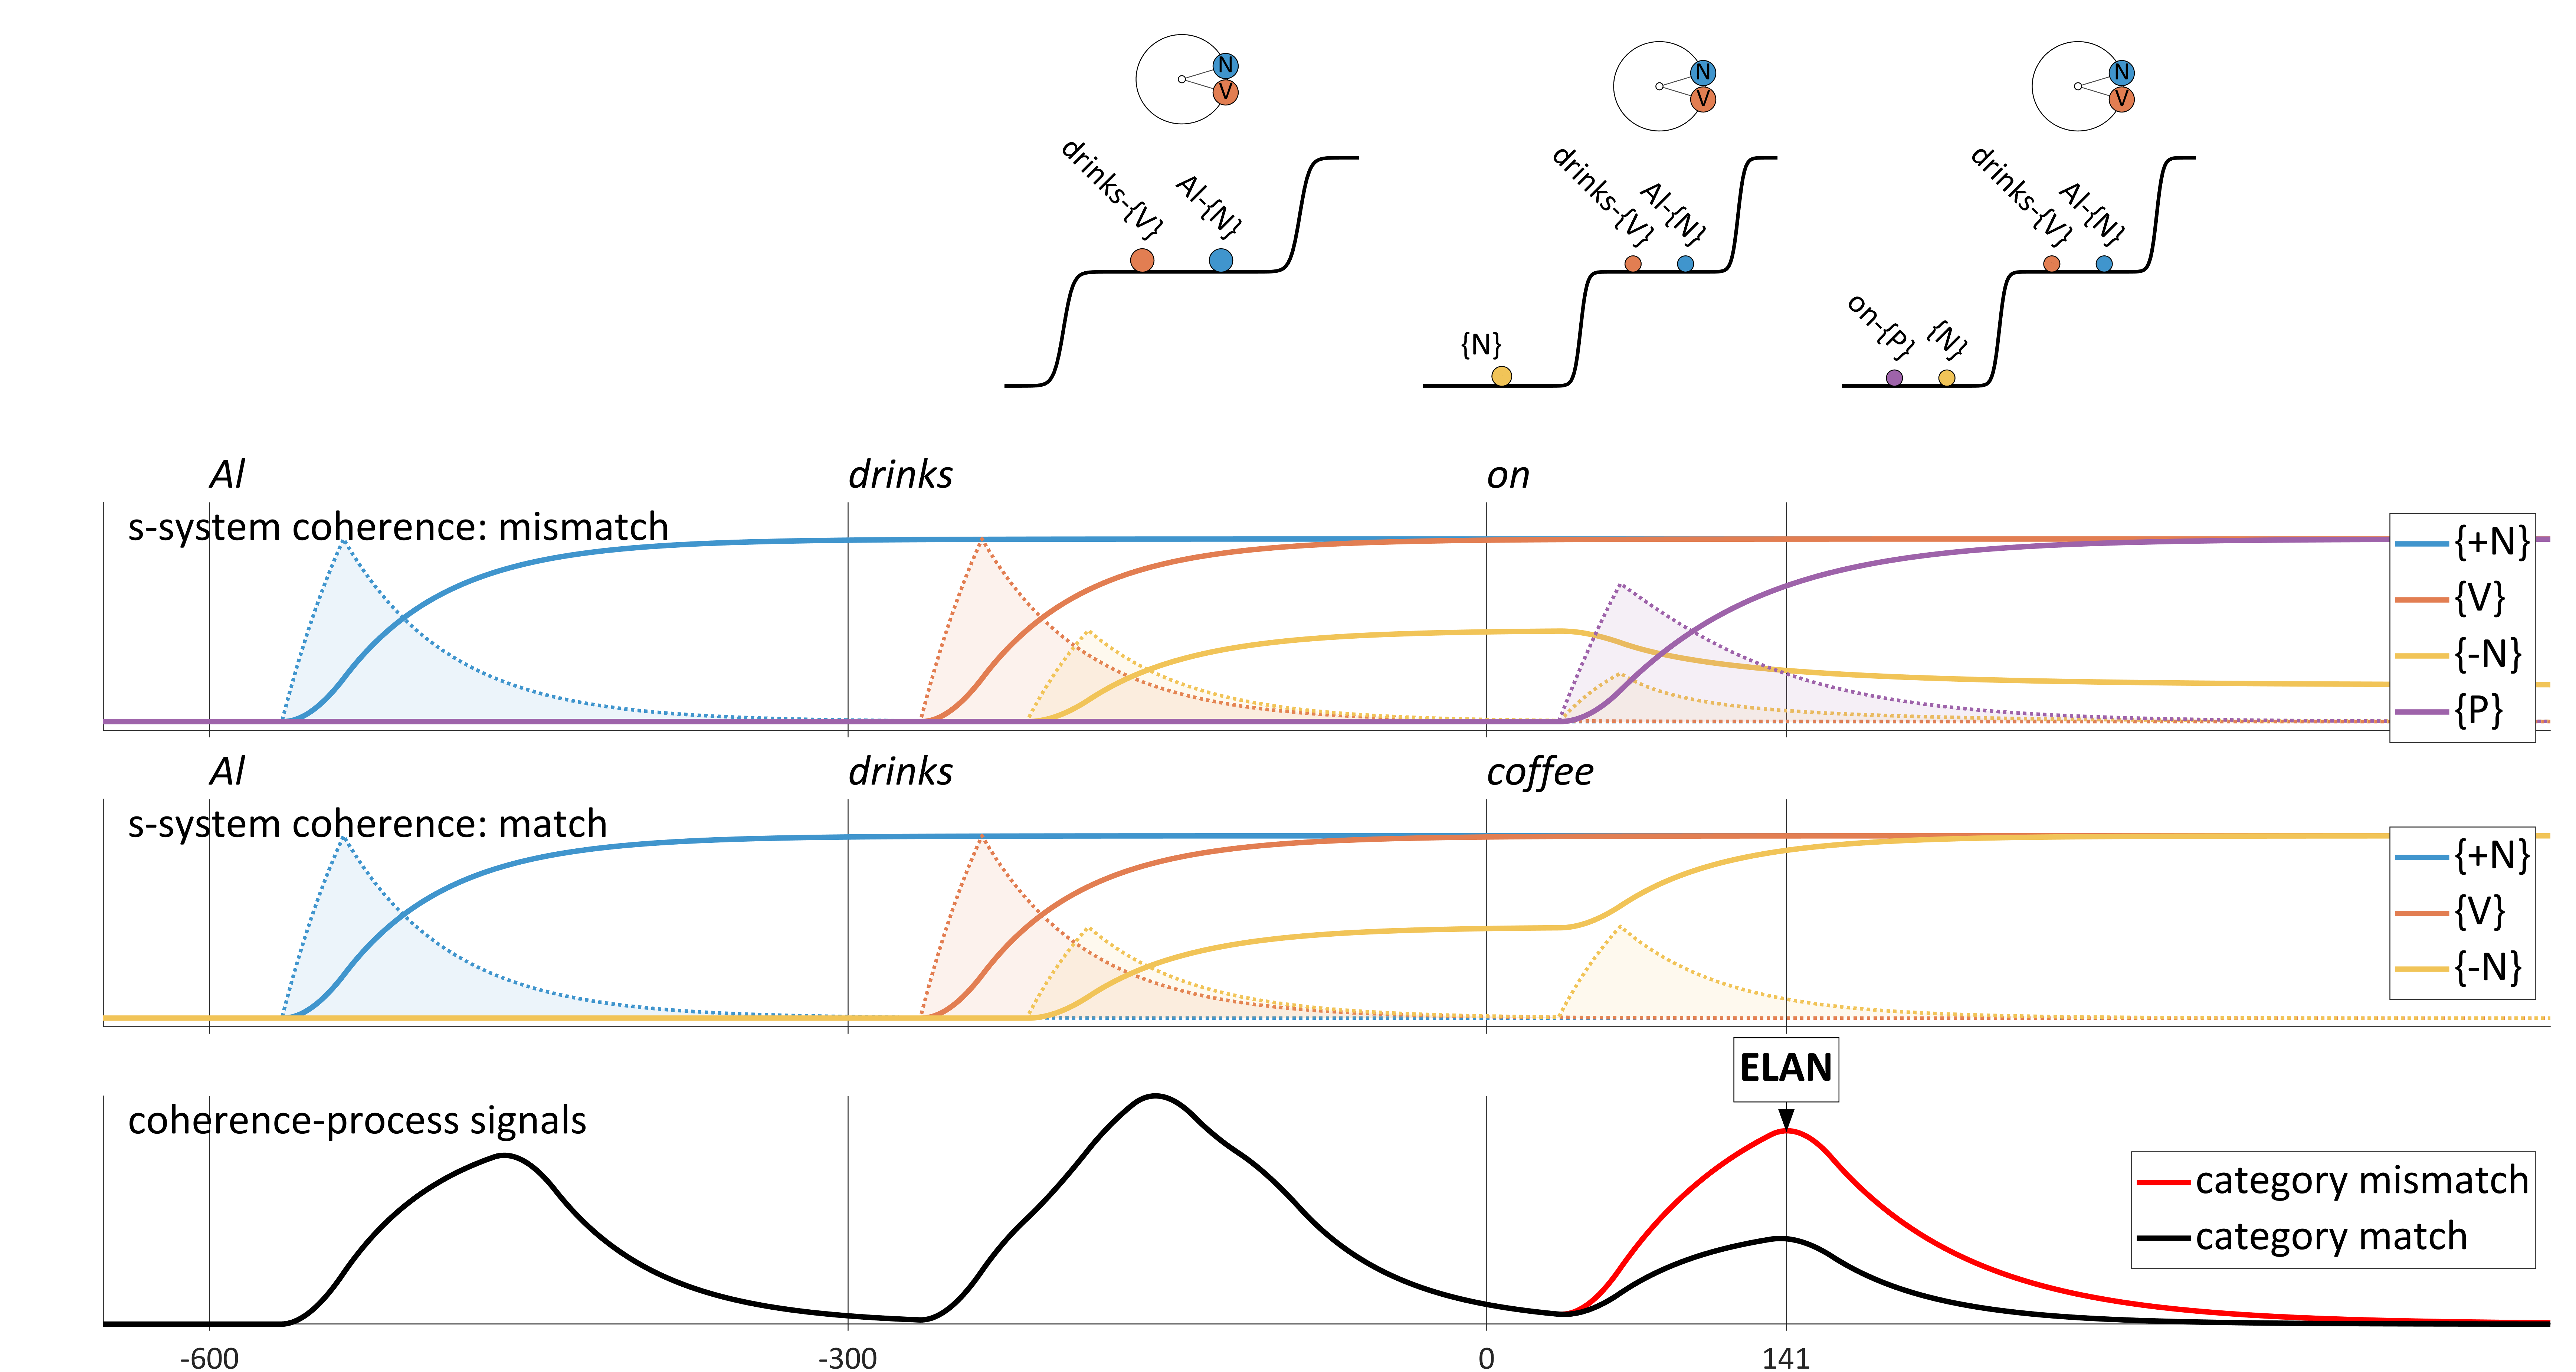
\includegraphics[width=\textwidth]{figures/Tilsen-img142.png}
\caption{Early left anterior negativity (ELAN): activation of less expected s-sys\-tem results in a larger coherence-process signal than activation of a more expected s-sys\-tem.}
\label{fig:6:23}
\end{figure}
 

There are several reasons why the \isi{coherence-process signal} after presentation of the mismatching category \{P\} is greater than the signal when the expected \{N\} is presented. Because the \{−N\} system is already activated, a smaller increase in \isi{coherence} is required to achieve an \isi{excited state} when \textit{coffee} is presented compared to the increase required for the \{P\} system to reach a coherent state when the \isi{preposition} \textit{on} is presented. Hence one source of the ERP effect is that excitation of \{P\} requires a greater change of \isi{coherence}, and as elaborated above, coherence-process signals reflect an integration of changes in \isi{coherence}. Another possible source of the ERP effect may be \isi{interference} between \{P\} and \{−N\}. This \isi{interference} is expected to slow achievement of \isi{coherence} of \{P\} and possibly decrease the \isi{coherence} of \{−N\} -- these effects are illustrated in {\figref{fig:6:23}} as well. An increase in the period of time over which \isi{coherence} is achieved, and a change in the \isi{coherence} of the already active \{−N\}, both contribute to a larger \isi{coherence-process signal}.

  The next ERP we consider is the \isi{N400}, which is a negative peak observed from 300-500 ms after stimulus presentation. The amplitude of the \isi{N400} is inversely correlated with the extent to which a word is semantically expected (\citealt{FedermeierLaszlo2009,Friederici2002,KutasFedermeier2011}). For example, the c-sys\-tem [coffee] which is activated by utterance \REF{ex:6:24a} is more expected than the c-sys\-tem [toothpaste] activated in \REF{ex:6:24b}. The word \textit{coffee} has a greater cloze probability than \textit{toothpaste} in this context, i.e. a greater likelihood of completing the sentence \textit{Al drinks}.

\ea\label{ex:6:24}
\ea\label{ex:6:24a} Al drinks coffee. \break concept more consistent with expectations: smaller \isi{N400}
\ex\label{ex:6:24b} Al drinks toothpaste. \break concept less consistent with expectations: larger \isi{N400}
\z
\z

The analysis of the \isi{N400} is directly parallel to the analysis of the ELAN: [coffee] is primed by [drinks] to a greater extent than [toothpaste], and hence the achievement of \isi{coherence} of [toothpaste] requires a greater change in \isi{coherence} than [coffee]. The key difference between the ELAN and the \isi{N400} is that the ELAN arises from activation of s-sys\-tems, while the \isi{N400} arises from activation of c-sys\-tems. As described above, c-sys\-tem excitation is delayed relative to s-sys\-tem excitation, because c-sys\-tem excitation requires resonance with an excited s-sys\-tem.

  
\begin{figure}
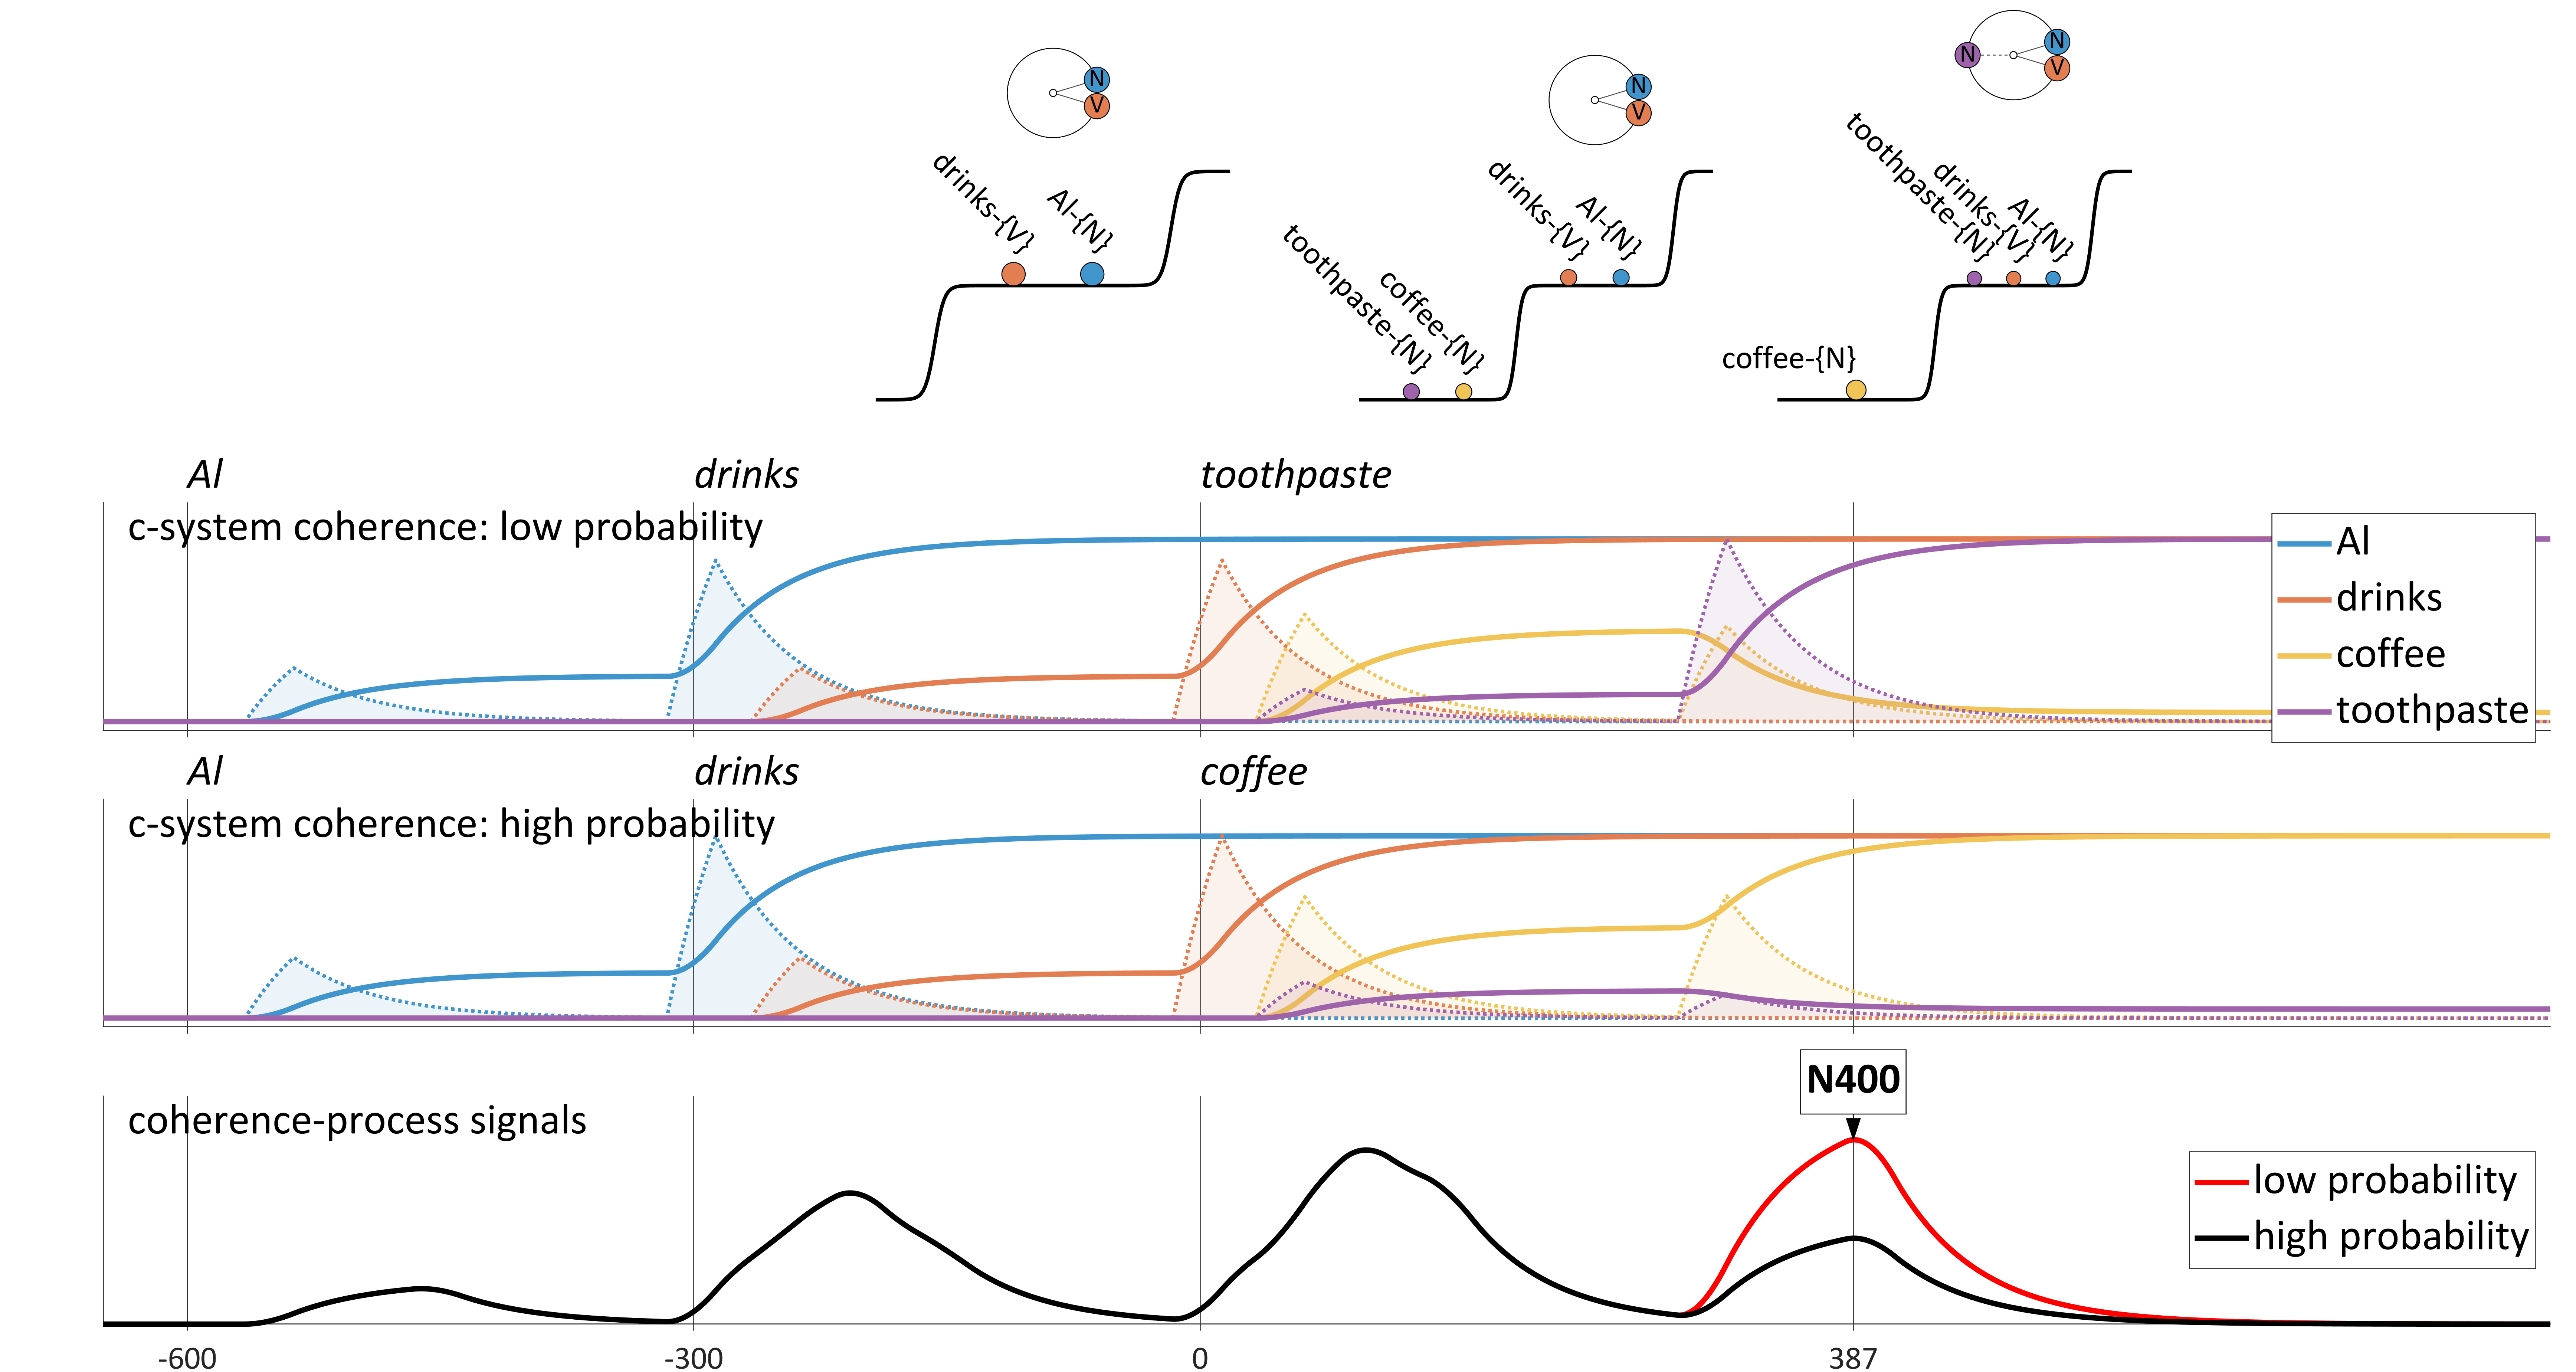
\includegraphics[width=\textwidth]{figures/Tilsen-img143.png}
\caption{N400: activation of less expected c-sys\-tem results in a larger coherence process signal than activation of a more expected c-sys\-tem.}
\label{fig:6:24}
\end{figure}
 

The \isi{N400} effect does not require a sentential context and is influenced by a number of factors which include semantic category membership, word frequency, and neighborhood density (\citealt{KutasFedermeier2011,LauEtAl2008}). In lists of words in which a semantic category expectancy is generated, a word whose semantic category deviates from the expectation will induce a larger \isi{N400}. For example, in the utterances in \REF{ex:6:25}, \textit{toothpaste} will induce a larger \isi{N400} than \textit{wine}. The \isi{N400} is sensitive to word frequency as well: in the utterances in \REF{ex:6:26}, \textit{ouzo} will induce a larger \isi{N400} than \textit{coffee}. In both cases, it is sensible to assume that prior to presentation of the stimulus \textit{wine}, a [wine] system is already active to some degree, and hence a smaller change in \isi{coherence} of [wine] occurs post-stimulus than in cases where the stimulus-activated c-sys\-tem has been pre-activated to a lesser degree. In other words, the frequency effect arises because [drinks] activates (“primes”) a higher-frequency c-sys\-tem like [wine] to a greater extent than a lower-frequency c-sys\-tem like [ouzo].

\ea\label{ex:6:25}
\ea\label{ex:6:25a} coffee, tea, whisky, wine
\ex\label{ex:6:25b}  coffee, tea, whisky, toothpaste
\z
\z

\ea\label{ex:6:26}
\ea\label{ex:6:26a} Al drinks wine.
\ex\label{ex:6:26b} Al drinks ouzo.
\z
\z

  The interpretation of neighborhood density effects on the \isi{N400} is somewhat different from the effects discussed above. A word with a denser neighborhood will induce a larger \isi{N400} than a word with a sparser neighborhood \citep{HolcombEtAl2002,MüllerEtAl2010}. This effect should be understood to arise because stimuli with denser neighborhoods will activate more c-sys\-tems than those with sparser neighborhoods. When more c-sys\-tems are active, there is more competition between c-sys\-tems for a cs-resonance and the c-sys\-tems interfere with each other to a greater extent. Hence it will take longer for a coherent cs-resonance to emerge than in a condition where fewer c-sys\-tems are primed. 

  An interesting finding regarding the \isi{N400} is that it is often insensitive to negation \citep{KutasFedermeier2011}. Hence N400s for \textit{toothpaste} are similar in \textit{Al drinks toothpaste} and \textit{Al do not drink toothpaste}. This suggests that negation and possibly quantification in general does not influence the priming effects that modulate the amplitude of the \isi{N400}. This raises questions regarding \isi{relational meaning} experiences which involve negation and quantification; an analysis of such meaning experiences has not yet been developed in the o/el framework.

  In the same time period as the \isi{N400}, a left anterior negativity (LAN) is sometimes observed in response to \isi{morphosyntactic} agreement violations (\citealt{Friederici2002,GunterEtAl2000,KutasFedermeier2011,OsterhoutHolcomb1992}). For example, \textit{the students drinks coffee}, where the verbal number agreement mismatches the number of the subject argument, will elicit a greater \isi{N400} than \textit{the student drinks coffee}. This suggests that excitation of grammatical s-sys\-tems (i.e. \{\textsc{number}\}, \{\textsc{person}\}, \{\textsc{tense}\} etc.) occurs later in time than excitation of lexical s-sys\-tems (i.e. \{N\}, \{V\}, \{P\}, etc.), where expectation mismatches are associated with the ELAN. This is consistent with the notion that grammatical s-sys\-tems must be coupled to excited lexical s-sys\-tems in order to become excited themselves. This accords with the idea that the utterance \textit{the}, which excites only \{D\}[\textsc{definite}], does not give rise to a coherent configuration: there is no lexical cs-resonance for \{D\}[\textsc{definite}] to couple with. It should be noted, however, that agreement violations do not always appear to elicit a LAN effect, but instead may elicit a later effect called the \isi{P600}, which we consider next. In these cases, both prior syntactic and conceptual excitation may be required for effects to manifest in coherence-process signals.

  The \isi{P600} is a positive EEG signal occurring from 600-1000 ms after a stimulus. The \isi{P600} has a centro-parietal location, as opposed to the left-anterior locations of the ELAN and LAN. It has been associated with syntactic violations, processes of reanalysis and repair (as in garden-path sentences), and syntactic complexity \citep{Friederici2002}. Although some researchers view the \isi{P600} as a language-specific ERP component, others have argued that the \isi{P600} is not distinct from the more general P3, an ERP that is associated with attention-related reorientation behavior \citep{SassenhagenBornkessel-Schlesewsky2015}. This raises the question of whether in the o/el model the \isi{P600} (or P3) can be understood differently from the ELAN, \isi{N400}, and LAN, all of which are attributable to priming, i.e. pre-stimulus activation of systems below the excitation threshold.

  To address this, let's consider a \isi{garden path} sentence such as \textit{Al drinks coffee and tea is brewing}. Assume that in the garden-path interpretation there is a state in which an {\textbar}Al drinks coffee{\textbar} configuration is excited, followed by a state in which an {\textbar}Al drinks tea{\textbar} configuration is excited. Upon occurrence of the stimuli \textit{is brewing}, the relevant cs-sys\-tems [be]\{\textsc{aux}\} and [brew]\{V\} become active, but because [tea]\{N\} is already coupled to [drink]\{V\}, [tea]\{N\} is not able to couple stably to [brew]\{V\}. This results in [brew]\{V\} failing to achieve \isi{coherence}. We conjecture that this non-\isi{coherence} induces a “repair” process, which involves selectively grounding e-operations and subsequent reorganization operations. If the reorganization leads to a grammatically coherent trajectory, the repair is successful. However, the grounding and reorganization e-operations that occur during the repair result in many changes in spectral and cross-\isi{spectral coherence}, which are manifested as changes in EEG power. This is illustrated in {\figref{fig:6:25}}.

  
\begin{figure}
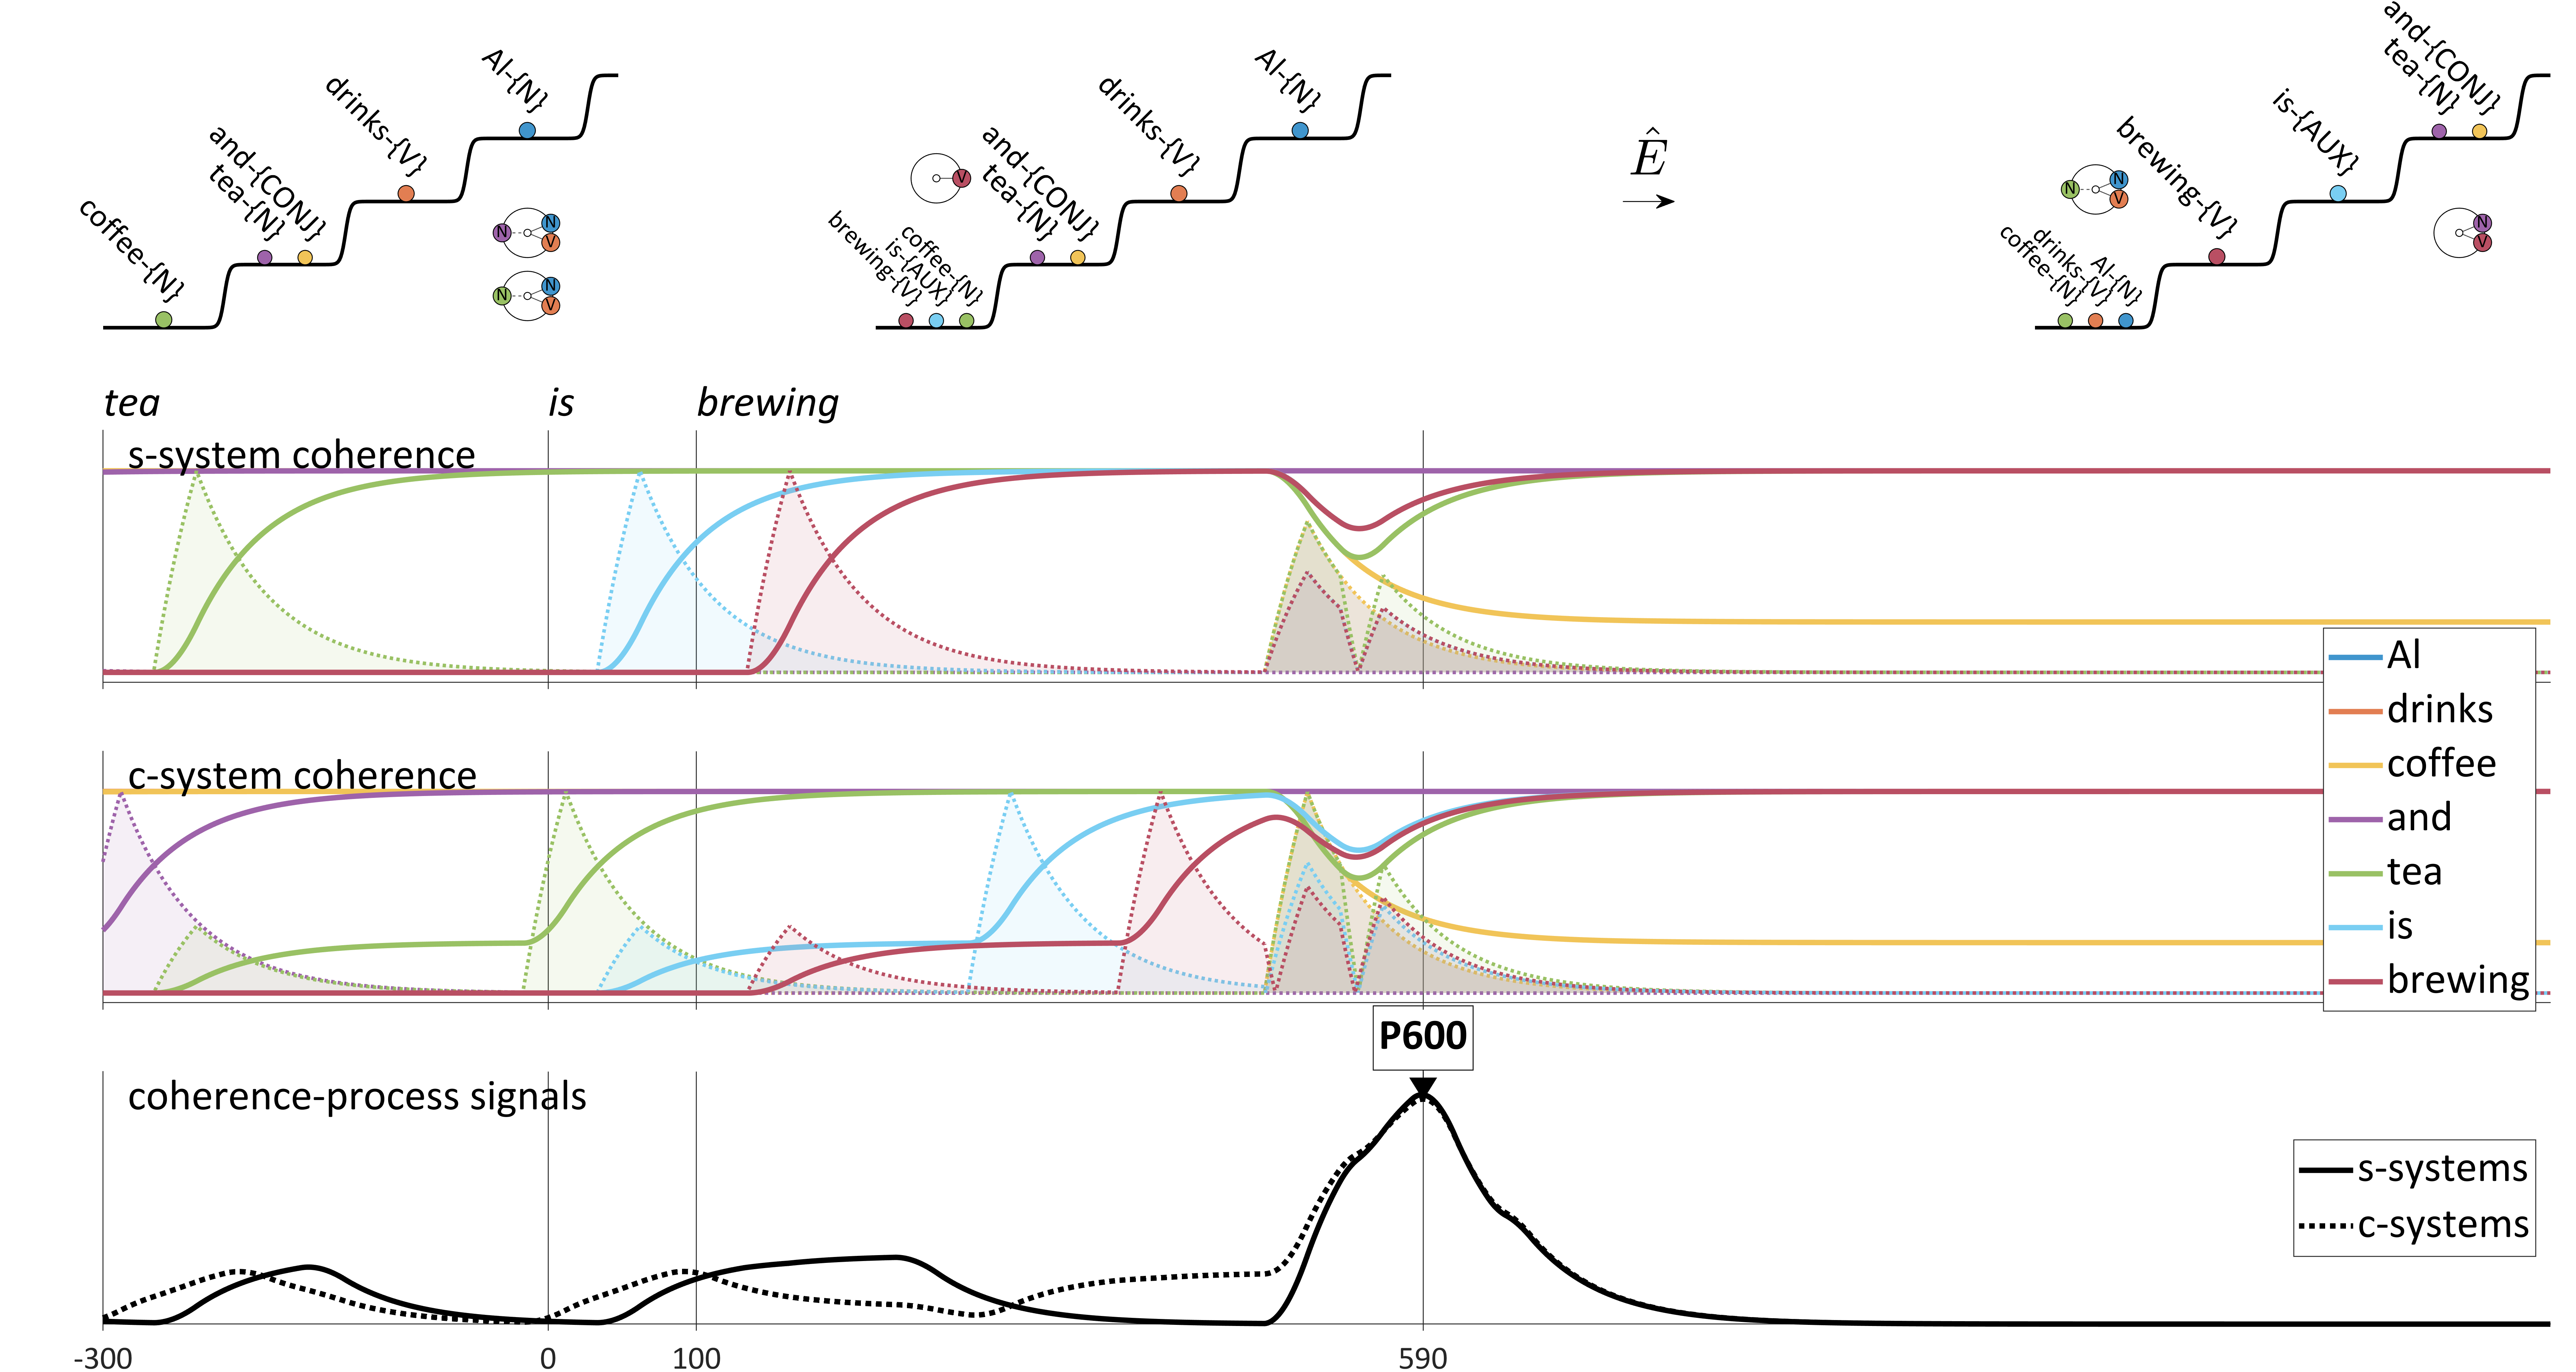
\includegraphics[width=\textwidth]{figures/Tilsen-img144.png}
\caption{P600 in a garden-path interpretation: detection of non-coherence and reorganizations for repair result in a large coherence-process signal.}
\label{fig:6:25}
\end{figure}
 

One question we might ask is why the \isi{P600} has a different spatial distribution and sign than other ERPs. Consider that there are several differences in the mechanisms which cause \isi{coherence} changes during a repair, compared to those associated with priming effects. For starters, the ELAN and \isi{N400} are associated with the timecourse of excitation of cs-sys\-tems, which occurs prior to the emergence of a stable configuration; this excitation does not necessitate any e-or\-ga\-ni\-za\-tion. In contrast, the \isi{P600} is associated with e-operations on already-excited or already-activated systems, and hence is expected to occur later. Secondly, it may be useful to construct \textit{coherence-response systems}, which are systems which become active when cs-states are non-coherent. Coherence response systems provide a mechanism for “monitoring” the state of the system, and likely play a role in shaping \isi{grammaticality} intuitions discussed earlier. It would not be surprising if \isi{coherence} response systems have a different spatial distribution than cs-sys\-tems, but the imprecision in spatial localization of ERP generators warrants caution in drawing inferences in this regard.

\subsection{Toward a new vocabulary of psycholinguistic analysis}

The o/el framework offers an alternative vocabulary for interpreting \isi{psycholinguistic} observations of behavior. There are several advantages of this vocabulary: (i) It brings temporal phenomena to the fore with a conceptual model that is focused on dynamics. (ii) It avoids potentially misleading anthropomorphizations. (iii) It provides a basis for a more specific conception of \textit{information}. (iv) It avoids conceptual dissonance that arises in describing phenomena which necessitate simultaneous reference to incompatible structures.

To illustrate these advantages, let's consider how ERP effects are typically described in \isi{psycholinguistic} literature. Such effects are commonly attributed to “mismatches,” “processing difficulty,” or “reanalysis/repair” (see e.g. \citealt{Friederici2002,KutasFedermeier2011}). For instance, the ELAN is understood as the result of a mismatch between the \isi{syntactic category} of a stimulus and the expected category, which occurs in a process of word category “identification”. The \isi{N400} is understood as an index of difficulty in “processing” which occurs in the “integration” of semantic and syntactic “information”. The \isi{P600} is understood as an index of complexity or the need for “reanalysis”.

Psycholinguistic studies do not always provide more specific details regarding what these terms mean in the context of a conceptual model of syntax. Basic questions arise which call for detailed answers: what is “processing”? What does it mean to “identify” a \isi{syntactic category}? What form does the “expectation” of a category take? What is a “category”, anyway? Object-based conceptions do not readily help us understand the behavioral manifestations of processing, because objects are \isi{atemporal}. In contrast, the systems of the o/el framework evolve in time and are characterized in terms of states. Thus “identification” of a category can be understood as a \isi{state space} trajectory in which sensory systems activate conceptual and syntactic systems, and in which those systems subsequently evolve from an active state to an \isi{excited state}, via coupling/resonance mechanisms. The microscale conceptual model further informs our understanding of the trajectory by allowing us to think of the evolution as emergence of spectrally coherent collective oscillations in neural populations. The \textit{trajectory} IS the “processing,” and there are no categories, but rather, \textit{systems}.

The concept of “processing information” is potentially misleading for a couple reasons. First, \textit{processing} evokes a computational interpretation of phenomena, and most computational models impose temporally discrete operations on system states. The states of systems we have constructed are understood to evolve continuously in the \isi{pre-stable phase} of trajectories, and this evolution should not be viewed as the consequence of discrete operations. Of course, discrete computations applied in the limit of infinitesimally small time increments provides an effectively continuous approximation to system dynamics, but computational interpretations in linguistic theories rarely adopt this infinitesimal limit construal. Thus use of the word \textit{processing} has the potential to evoke a counterproductive discretization of time in pre-stable phases of system state trajectories. Second, the computational interpretation tends to evoke symbols, because many computational models of language are developed to manipulate symbolic representations, rather than states defined in continuous dimensions. Because symbols are objects, any interpretation of behavior which evokes them will lead to many of the problems of the \isi{object metaphor} which we have discussed in this book. 

In a deeper sense, the interpretation of information processing as symbol manipulation unnecessarily obscures the nature of the \isi{state space} and thereby leads to an inadequate conception of \textit{information}. What do people mean when they say that the brain “processes information”? The word \textit{information} seems to be often used in a non-technical sense, and is rarely defined in a rigorous manner. The tenets of information theory \citep{Shannon1948} hold that information is \textit{produced} when a previously undetermined (or unobserved) system state is determined (or observed). The information produced by the determination process is measured as the change in entropy (H) of the system from before determination to after determination. The entropy is the negative sum of the log probabilities of states, weighted by their probabilities, as shown in the equation below. Thus information is entropy lost in the determination of a system state.

\ea
  Information produced = Entropy before – Entropy after
$$
H=-\sum _{i} p_i \log \left(p_i\right) = -p_1 \log \left(p_1\right) - p_2\log \left({p}_{2}\right) - \dots - p_n\log \left({p}_{n}\right)
$$
\z

In the case of a system which generates equiprobable discrete states, such as a coin flip or a random selection of a character from the alphabet, the information that is produced from each flip or character selection (i.e. from the determination process), increases when there are more possible states: hence there is more information produced by selecting a character of the alphabet than by flipping a coin. In both cases, the entropy after determination is zero -- the system state is fully determined, but the number of possible states before determination is greater for the alphabet, which has 26 possible states, than for the coin, which has only 2. The same reasoning can be generalized to continuous variables, in which case it is the probability-weighted volume of the \isi{state space} before determination that matters for calculating the information that is produced. It is crucial to recognize that a state of the system itself does not “have information,” but rather, information is something that is “gained” by a reduction of volume of the \isi{state space} or “lost” by an increase of volume of the \isi{state space}. Furthermore, the first terms in the products in the entropy equation, which are probabilities of states ($p_i$), are weighting terms which specify how much each sub-volume of \isi{state space} contributes to the total entropy associated with the space. The information gained by determination of a state is maximal when those probabilities are uniformly distributed over the space.

How does the technical understanding of information gel with the o/el conception of a \isi{state space} trajectory? The o/el analysis might seem to imply that no information can ever be lost or gained: the system state is always determined, and evolves according to deterministic laws; thus there is no determination process which allows for a change in entropy. However, consider that our analyses always partition the full system state into systems and a \isi{surroundings}: it is only the systems whose states are always determined; the \isi{surroundings} state is never determined. Hence entropy can be transferred from systems to the \isi{surroundings}. Indeed, this is exactly what happens on the microscale when a c-sys\-tem or s-sys\-tem becomes active: the entropy of the population decreases, by means of being transferred to the \isi{surroundings}. This entails a reduction in the number of accessible microstates of the system, but not of the universe.

Alternatively, we can say that the order (i.e. negentropy, see \citealt{Schrödinger1944}) of the system increases. Thus information has been produced \textit{locally}, i.e. in the region of \isi{state space} which is relevant to describing the system. This local increase is always offset by an increase of entropy in the \isi{surroundings}, and according to the second law of thermodynamics is always greater than or equal to the local decrease. It is more appropriate, in o/el terms, to think of “information processing” as local increase or decrease of order in systems. The advantages of this perspective are that we allow for a more detailed accounting of the temporal evolution of probability mass in \isi{state space}, and are better able to see the connection between information and our analytical choices in partitioning the universe into systems vs. \isi{surroundings}. 

Another advantage of the o/el conception is that “expectation” or “prediction” of a category or meaning are not associated with an ad hoc, anthropomorphic mechanism. Instead, a more phenomenologically neutral description is available in which the activation of a system induces activation of other systems which are likely to become active in the future. This mechanism allows us to understand ELAN, LAN, and \isi{N400} effects just as readily as conventional vocabularies. “Prediction” is problematic because it evokes a potentially misleading anthropomorphization of the system. The verb \textit{predict} entails an animate agent (cf. \textit{Bo predicted Al would drink coffee} vs. \textsuperscript{?}\textit{The table predicted Al would drink coffee}). There is no theoretical necessity to conceptualize the system as animate, or as the sort of entity which “makes predictions”. Rather, we say that the system state evolves such that its location in \isi{state space} tends to move closer to states which are statistically more likely to arise in the future. This aspect of the system is a consequence of supra-utterance scale “learning” mechanisms which are viewed microscopically as changes in within- and between-population interactions.

The conventional vocabulary often employs terms like \textit{reanalysis} or \textit{repair}. But what is being reanalyzed, and what entity is doing the reanalyzing? In some cases authors propose to interpret these terms with object-based representations. For example, reanalysis has been described with substitution and adjunction operations on elementary trees in a tree-adjoining grammar conception \citep{FFerreiraEtAl2004}. Thus reanalysis involves the unmerging of some objects, while keeping those objects present, in order to re-merge them subsequently. One problem with this sort of conceptualization is that is does not predict any inherent cost for the “floating structures” or “unintegrated objects” which arise in such models, nor for the operations which create them. Why should object structures which are not connected to other object structures be problematic? It is certainly possible in such models to stipulate that unmerged objects give rise to processing difficulty, but this does not address the question of \textit{why} the processing difficulty arises, or what “processing” is in a mechanistic sense.

The o/el framework provides greater clarity regarding what processing is,\linebreak what “unintegrated structures” are, and why the reanalysis that produces them leads to behavioral effects such as increased \isi{P600}, slowed reading times, and/or saccadic backtracking. In conventional approaches, unintegrated structures are structures of objects that are not merged into some other structure which is already present. Instead of imagining of objects in space, the o/el conception posits systems which can be characterized by their \isi{spectral coherence} and coupling to other systems. Unintegrated structures are cs-sys\-tems which are (i) not coupled to other cs-sys\-tems and (ii) are not spectrally coherent. A consequence of these conditions is that these systems experience stronger \isi{interference} from other systems, and are therefore less stable. The repair process, as described in our analysis of the \isi{P600}, involves the application of grounding and subsequent reorganization operations. This allows for alternative ϕ-con\-fi\-gu\-ra\-tions to arise, and subsequently for a grammatically coherent \isi{interpretation trajectory} to occur. The initial instability and the reorganization operations are associated with changes in \isi{spectral coherence} which manifest in ERPs. We have furthermore conjectured that there may be \textit{\isi{coherence} response systems} which respond to noncoherent states by inducing reorganizations. Along these lines, a sensible endeavor is to develop a model of oculomotor control in which \isi{coherence} response systems influence reading behavior; this will allow for reading time and saccadic backtracking to be modeled in the framework.

One of the most fundamental problems with object-based conceptions of \isi{psycholinguistic} phenomena is that they do not lend well to reasoning about the “parallel” activation of systems. Consider the \isi{garden path} utterance in \REF{ex:6:1ter} below. The \isi{interpreter} may excite a {\textbar}dressed baby{\textbar} configuration, but this leads to a non-coherent state because [played]\{V\} cannot participate in a ϕ-con\-fi\-gu\-ra\-tion with a \{+N\} system. The experience of non-\isi{coherence} may then induce reorganizations which lead to a coherent trajectory involving {\textbar}Al dressed (himself){\textbar} and {\textbar}baby played{\textbar} configurations. Psycholinguistic studies have found evidence that the garden-pathed \isi{relational meaning} of {\textbar}dressed baby{\textbar} may “linger,” based on the observation that interpreters will sometimes answer “yes” to question \REF{ex:6:2tera} \citep{SlatteryEtAl2013}, indicating that the originally engaged configuration remains in memory after the repair.

\ea\label{ex:6:1ter}
{While Al dressed the baby played in the crib.}
\z

\ea
\ea \label{ex:6:2tera} {Did Al dress the baby?}
\ex \label{ex:6:2terb }{Did Al dress himself?}
\z
\z

The issue here is how to conceptualize working memory and “lingering structures”. As we explored earlier, a standard mapping of the \isi{object metaphor} is that two linguistic units cannot occupy the same position in a structure, just as two different objects cannot occupy the same space. Thus in order to adapt a conventional conceptualization of structure to account for this sort of phenomenon, it is necessary to circumvent violations of the standard mapping. To wit, \citet{SlatteryEtAl2013} describe an account in which there is an “overlay function” which allows a lingering structure to be ‘present “underneath”’ the new structure. The fact that the authors scare-quote “underneath” suggests a subtle discomfort with the spatial implications of this metaphor, which are dissonant with the conventional conception. The lingering structure must be underneath the new one because objects cannot occupy the same space. But what is the nature of this new space that is underneath another space in which structures of objects can be “present”?

It is not the notion that interpretation involves parallel (i.e. simultaneous) activation of systems that is the problem, but rather, the notion that working memory is a space for objects. The problems are easily resolved when we see that our use of the term \textit{working memory} refers to certain aspects of a state (or dimensions of a \isi{state space}), rather objects occupying space. A working memory state can be defined in the same ϕ/e \isi{state space} as the one in which production and interpretation trajectories are defined. A “lingering structure” is a set of activated cs-resonances, which by virtue of being in an active state have an increased likelihood of being integrated into a stable configuration. These same systems may also prevent newly activated systems from participating in a configuration or may destabilize other systems.

The o/el framework thus provides an alternative vocabulary that, because of its emphasis on the dynamics of systems and construction of state spaces, clarifies our conception of information, avoids anthropomorphization, and links our conceptual model of language more directly to behavioral observations. The disadvantage of the alternative vocabulary is that it is unfamiliar. The only way to change that is to practice using the vocabulary, and thereby explore its utility for conceptualizing phenomena. To that end, the next chapter examines several syntactic phenomena which have received much attention in the conventional perspective.  

